\documentclass[dvips]{article}
\usepackage{graphics}
\setlength{\topmargin}{0mm}
\setlength{\textheight}{220mm}
\setlength{\oddsidemargin}{0mm}
\setlength{\textwidth}{160mm}

\begin{document}
\vspace{40mm}
\begin{center}
{\Large \bf{{\tt SENGA2} User Guide}}\\[5mm]
{\large Stewart Cant}\\[5mm]
{\large CFD Laboratory}\\[1mm]
{\large Department of Engineering, University of Cambridge}\\[1mm]
{\large Trumpington Street, Cambridge CB2 1PZ}\\[1mm]
{\large United Kingdom}\\[1mm]
{\large email: rsc10@cam.ac.uk}\\[7mm]
Report number CUED--THERMO--2012/04 (2nd ed.)\\[1mm]
November 2013
\end{center}

\newpage
\section{Introduction}
Direct Numerical Simulation (DNS) of turbulent combustion involves the
solution of the augmented Navier--Stokes equations without modelling of the
turbulence, and with an adequate treatment of the chemistry and the molecular
transport of momentum, heat and mass.  Ideally the chemical
reaction mechanism would be represented in fully detailed form, as
would the various mechanisms of molecular transport, and a separate
balance equation would be solved for the mass fraction of every chemical
species present in the reacting gas mixture.  Such a full treatment
remains computationally unaffordable for practical simulations,
and some degree of compromise is necessary in order to make progress. 

The {\tt SENGA2} code was derived from the earlier {\tt SENGA} code
\cite{JenkinsCant} which remains in use for DNS with simplified chemistry.  The
purpose of the {\tt SENGA2} code is to facilitate combustion DNS with any
desired level of chemistry, from single-step Arrhenius mechanisms through all
classes of reduced reaction mechanisms up to fully detailed reaction
mechanisms wherever this is feasible computationally.
Molecular transport can be represented using any type of Fickian
diffusion law or more complex treatments.  A simple treatment of radiation heat
transfer is included.  The Navier--Stokes momentum equations
are solved in fully compressible form together with the continuity
equation and a conservation equation for the stagnation internal energy,
as well as any required number of balance equations for species mass fraction.  
Each component of the reacting mixture is assumed to obey the equations of
state for a semi--perfect gas.  Boundary conditions are specified using
an extended form of the Navier--Stokes Characteristic Boundary Condition (NSCBC)
formulation \cite{PoinsotLele, SutherlandKennedy}, and available boundary
condition types include periodic as well as several varieties of walls,
inflows and outflows.

The numerical framework is based on a high--order finite--difference approach
for spatial discretisation together with a Runge--Kutta algorithm for
time--stepping.
Spatial differencing schemes are implemented in the code through a set
of modular spatial differentiator routines, and examples of those tested 
include Fourier spectral schemes and high--order Pad\'{e}
finite--difference schemes \cite{Lele}.
High--order explicit schemes are preferred due to their speed of
execution and ease of parallel implementation, and a 10th order explicit
scheme is standard for interior points.  The accuracy of the scheme is
reduced to 8th, 6th and 4th order as a non--periodic boundary is approached.
For time--stepping, the Runge--Kutta algorithm may be adjusted to have any
number of sub--steps in order to achieve the required order of accuracy.
Adaptive time--stepping is available with error control using an embedded
Runge--Kutta scheme.  The standard time--stepping algorithm is a
five--step fourth--order explicit Runge--Kutta method with a third--order
embedded scheme \cite{KennedyCarpenterLewis} together with
a PID--type time step controller \cite{KennedyCarpenter}.  The code is fully
parallel using domain decomposition over a Cartesian topology.

The chemical and thermodynamic data required for each simulation is
handled in a compact tabular form in order to maximise computational
efficiency during a simulation.  A pre--processor code called {\tt PPCHEM} is
available to convert the chemical and thermodynamic data from a simple
text--based format into the required form for input to {\tt SENGA2}.  Another
pre--processor code called {\tt PPDIFF} is available to convert the data
required to treat molecular transport using a mixture--averaged formulation. 

\section{Mathematical Formulation}
\subsection{Governing Equations}
The governing equations to be solved using DNS are the partial
differential equations for compressible reacting flow,
consisting of the continuity equation
\begin{equation}
\frac{\partial}{\partial t}\rho +
\frac{\partial}{\partial x_{k}}\rho u_{k} = 0,
\label{CONTINUITY}
\end{equation}
the Navier--Stokes momentum equations
\begin{equation}
\frac{\partial}{\partial t}\rho u_{i} +
\frac{\partial}{\partial x_{k}}\rho u_{k} u_{i} =
-\frac{\partial}{\partial x_{i}}p +
\frac{\partial}{\partial x_{k}} \tau_{ki},
\label{MOMENTUM}
\end{equation}
and the internal energy equation
\begin{equation}
\frac{\partial}{\partial t}\rho E +
\frac{\partial}{\partial x_{k}}\rho u_{k} E =
-\frac{\partial}{\partial x_{k}}p u_{k} -
\frac{\partial}{\partial x_{k}} q_{k} +
\frac{\partial}{\partial x_{k}} \tau_{km}u_{m} +
\dot{q}_{R},
\label{ENERGY}
\end{equation}
supplemented by an equation for the mass fraction of each of the $N$ chemical
species present in the reacting gas mixture
\begin{equation}
\frac{\partial}{\partial t}\rho Y_{\alpha} +
\frac{\partial}{\partial x_{k}}\rho u_{k} Y_{\alpha} =
w_{\alpha} -
\frac{\partial}{\partial x_{k}}\rho V_{\alpha,k} Y_{\alpha}.
\label{MASSFRAC}
\end{equation}
The thermal equation of state for the mixture is
\begin{equation}
p = \rho R^{0} T \sum_{\alpha=1}^{N} \frac{Y_{\alpha}}{W_{\alpha}}
\end{equation}
while the caloric equation of state provides the definition of the
stagnation internal energy as 
\begin{equation}
E = \sum_{\alpha=1}^{N} Y_{\alpha} h_{\alpha} - \frac{P}{\rho} +
\frac{1}{2}u_{k}u_{k}
\label{EOSCAL}
\end{equation}
where the enthalpy of species $\alpha$ is defined as
\begin{equation}
h_{\alpha} = \int_{T_{0}}^{T} C_{p\alpha} dT + h_{\alpha}^{0},
\label{ENTH}
\end{equation}
in which $C_{p\alpha}$ is the mass--based specific heat capacity of species
$\alpha$ and $h_{\alpha}^{0}$ is the species enthalpy at the reference
temperature $T_{0}$.  The viscous stress tensor is given by
\begin{equation}
\tau_{ki} = \mu\left(\frac{\partial u_{k}}{\partial x_{i}} +
\frac{\partial u_{i}}{\partial x_{k}}\right) -
\frac{2}{3}\mu\frac{\partial u_{m}}{\partial x_{m}}\delta_{ki},
\label{VISCSTRESS}
\end{equation}
In the energy equation (\ref{ENERGY}), the quantity $q_{k}$ is the heat flux
vector and is discussed in section \ref{SEC:MOLTRANS}, while the quantity
$\dot{q}_{R}$ is a radiation heat transfer term discussed in section
\ref{SEC:RADCAL}.
The species mass fractions are subject to the compatibility condition
\begin{equation}
\sum_{\alpha=1}^{N}Y_{\alpha} = 1
\label{COMPATY}
\end{equation}
while the diffusion velocities must satisfy the compatibility condition
\begin{equation}
\sum_{\alpha=1}^{N}\rho V_{\alpha,k}Y_{\alpha} = 0.
\label{COMPATV}
\end{equation}
For a reaction mechanism involving $M$ steps of the form
\begin{equation}
\sum_{\alpha=1}^{N}\nu_{\alpha,m}'{\cal M}_{\alpha} \rightarrow
\sum_{\alpha=1}^{N}\nu_{\alpha,m}''{\cal M}_{\alpha},\hspace{3mm} m=1,\ldots,M
\end{equation}
the chemical production rate $w_{\alpha}$ for species $\alpha$ is expressed as
\begin{equation}
w_{\alpha} = W_{\alpha}
\sum_{m=1}^{M}\left(\nu_{\alpha,m}''-\nu_{\alpha,m}'\right)k_{m}(T)
\prod_{\beta=1}^{N}c_{\beta}^{\nu_{\beta,m}'}.
\label{RRATE}
\end{equation}
where the specific reaction rate coefficient $k_{m}(T)$ is given by
the Arrhenius expression 
\begin{equation}
k_{m}(T) = A_{m}T^{n_{m}}\exp{\left(-\frac{E_{m}}{R^{0}T}\right)}
\label{KRATE}
\end{equation}
and the concentration $c_{\beta}$ of species $\beta$ is related to
mass fraction by
\begin{equation}
c_{\beta} = \frac{\rho Y_{\beta}}{W_{\beta}}.
\label{CONCDEF}
\end{equation}
For the reaction rates the compatibility condition is
\begin{equation}
\sum_{\alpha=1}^{N}w_{\alpha} = 0.
\label{COMPATW}
\end{equation}

\subsection{Thermodynamic Quantities}
For a semi--perfect gas, the molar specific heat capacity at constant pressure
$\bar{C}_{p\alpha}$
is known to depend on temperature, and for present purposes the dependence is 
represented in an approximate manner using a polynomial of the form
\begin{equation}
\frac{\bar{C}_{p\alpha}}{R^{0}}
= \sum_{j=1}^{J} \bar{a}_{\alpha,j}^{(l)}T^{j-1}
\label{CPPOLY}
\end{equation}
where the degree $J-1$ of the polynomial is typically taken to be 4 or 5.
The polynomial coefficients $a_{\alpha,j}^{(l)}$ may take different values
for each species $\alpha$ in different intervals $l$ of temperature.
For example, the popular CHEMKIN database \cite{Chemkin} uses
polynomials of degree 5 with two temperature
intervals: for most species the intervals are $0 < T < 1000{\rm K}$ ($l$ = 1)
and $1000{\rm K} \le T < 3000{\rm K}$ ($l$ = 2).  The molar enthalpy
for each species is
given by integrating over $L$ successive temperature intervals
$l=1,\ldots,L$ to yield the recursive formula
\begin{eqnarray}
\bar{h}_{\alpha}
& = & R^{0}\int_{T_{L-1}}^{T} \sum_{j=1}^{J} \bar{a}_{\alpha,j}^{(L)}T^{j-1}dT
+ R^{0}\sum_{l=1}^{L-1}\left[
\int_{T_{l-1}}^{T_{l}}\sum_{j=1}^{J}\bar{a}_{\alpha,j}^{(l)}T^{j-1}dT
\right]
+ \bar{h}_{\alpha}^{0} \nonumber\\
& = & R^{0}\sum_{j=1}^{J} \frac{\bar{a}_{\alpha,j}^{(L)}}{j}T^{j} -
R^{0}\sum_{j=1}^{J} \frac{\bar{a}_{\alpha,j}^{(L)}}{j}T_{L-1}^{j} +
\bar{h}_{\alpha}^{(L-1)}.
\end{eqnarray}
where the reference temperature $T_{0}$ has been taken at 0K, and 
$h_{\alpha}^{(L-1)}$ denotes the enthalpy at the lower end of the current
($L$th) temperature interval.
The last two terms may be combined to form a single coefficient
$\bar{a}_{\alpha,J+1}^{(L)}$, and the final form for the molar enthalpy
becomes
\begin{equation}
\bar{h}_{\alpha} = R^{0}\left[
\sum_{j=1}^{J} \frac{\bar{a}_{\alpha,j}^{(L)}}{j}T^{j}
+ \bar{a}_{\alpha,J+1}^{(L)}
\right]
\label{ENTHMOL}
\end{equation}
Similarly, the molar entropy for each species may be found using the definition
\begin{equation}
\bar{s}_{\alpha} = R^{0}\int_{T_{0}}^{T} \frac{\bar{C}_{p\alpha}}{T} dT
+ \bar{s}_{\alpha}^{0}, 
\end{equation}
substituting for $\bar{C}_{p\alpha}$ and integrating over successive
temperature intervals to give
\begin{eqnarray}
\bar{s}_{\alpha}
& = & R^{0}\left[
\bar{a}_{\alpha,1}^{(L)}\ln{T}
+ \sum_{j=2}^{J} \frac{\bar{a}_{\alpha,j}^{(L)}}{j-1}T^{j-1}
\right]\nonumber\\
& - & R^{0}\left[
\bar{a}_{\alpha,1}^{(L)}\ln{T_{L-1}} +
\sum_{j=2}^{J} \frac{\bar{a}_{\alpha,j}^{(L)}}{j-1}T_{L-1}^{j-1}\right] +
\bar{s}_{\alpha}^{(L-1)}
\end{eqnarray}
where once again the formula may be applied recursively, and
$s_{\alpha}^{(L-1)}$ is the entropy at the lower end of the current
temperature interval.
Combining the last three terms to form a single coefficient
$\bar{a}_{\alpha,J+2}^{(L)}$, the final form for the molar entropy is
\begin{equation}
\bar{s}_{\alpha} = R^{0}\left[
\bar{a}_{\alpha,1}^{(L)}\ln{T} +
\sum_{j=2}^{J} \frac{\bar{a}_{\alpha,j}^{(L)}}{j-1}T^{j-1}
+ \bar{a}_{\alpha,J+2}^{(L)}
\right]
\label{ENTRMOL}
\end{equation}
The mass-based specific heat capacity $C_{p\alpha}$ is given by
\begin{equation}
C_{p\alpha}
= \frac{R^{0}}{W_{\alpha}}\sum_{j=1}^{J} \bar{a}_{\alpha,j}^{(l)}T^{j-1}
= \sum_{j=1}^{J} a_{\alpha,j}^{(l)}T^{j-1}
\end{equation}
where the mass-based polynomial coefficients are defined as
\begin{equation}
a_{\alpha,j}^{(l)} = \frac{R^{0}}{W_{\alpha}} \bar{a}_{\alpha,j}^{(l)}.
\end{equation}
Then the mass-based specific enthalpy for each species is
\begin{equation}
h_{\alpha} = 
\sum_{j=1}^{J} \frac{a_{\alpha,j}^{(L)}}{j}T^{j}
+ a_{\alpha,J+1}^{(L)}
\label{ENTHMAS}
\end{equation}
and the mass-based specific entropy for each species is
\begin{equation}
s_{\alpha} =
a_{\alpha,1}^{(L)}\ln{T} +
\sum_{j=2}^{J} \frac{a_{\alpha,j}^{(L)}}{j-1}T^{j-1}
+ a_{\alpha,J+2}^{(L)}.
\label{ENTRMAS}
\end{equation}

\subsubsection{Temperature}
The temperature may be obtained using the caloric equation of state
(\ref{EOSCAL}) in the form
\begin{equation}
E = \sum_{\alpha=1}^{N} Y_{\alpha} h_{\alpha} - R_{m}T +
\frac{1}{2}u_{k}u_{k}
\end{equation}
where the specific gas constant for the mixture is 
\begin{equation}
R_{m} = \sum_{\alpha=1}^{N} Y_{\alpha} R_{\alpha}.
\end{equation}
Substituting the polynomial form of the species enthalpy $h_{\alpha}$
from (\ref{ENTHMAS}) gives
\begin{equation}
E = \sum_{\alpha=1}^{N} Y_{\alpha}\left[
\sum_{j=1}^{J} \frac{a_{\alpha,j}^{(l)}}{j}T^{j} + a_{\alpha,J+1}^{(l)}
\right] - R_{m}T + \frac{1}{2}u_{k}u_{k}
\end{equation}
and gathering terms in successive powers of $T$ produces the polynomial
\begin{eqnarray}
f(T) & = & \left[
\left(\frac{1}{2}u_{k}u_{k} - E\right)
+ \sum_{\alpha=1}^{N} Y_{\alpha}a_{\alpha,J+1}^{(l)}
\right]\nonumber\\
& + & \left[
\sum_{\alpha=1}^{N} Y_{\alpha}\left(a_{\alpha,1}^{(l)}-R_{\alpha}\right)
\right]T
+\sum_{j=2}^{J}\left[
\sum_{\alpha=1}^{N} Y_{\alpha}\frac{a_{\alpha,j}^{(l)}}{j}
\right]T^{j}
\label{TEMPERPOLY}
\end{eqnarray}
which may be used to form the non-linear algebraic equation $f(T)=0$ whose
solution determines the temperature.

\subsection{Molecular Transport}
\label{SEC:MOLTRANS}
\subsubsection{Constant Lewis Numbers}
By default, the molecular transport coefficients are represented using
the relationship \cite{SmookeGiovangigli}
\begin{equation}
\frac{\lambda}{C_{p}} = A_{\lambda}\left(\frac{T}{T_{0}}\right)^{r}
\label{TRANSRELAT}
\end{equation}
for the mixture thermal conductivity $\lambda$, where $C_{p}$ is the
mixture value of the specific heat capacity at constant pressure,
and $A_{\lambda}$,
$r$ and $T_{0}$ are constants.  Then the mixture dynamic viscosity $\mu$
is given by
\begin{equation}
\mu = \frac{\lambda}{C_{p}}{\rm Pr}
\label{VISCRELAT}
\end{equation}
where ${\rm Pr}$ is the mixture Prandtl number which is taken as a constant.
\\[2mm]

\noindent
The diffusive mass flux for species $\alpha$ may be represented using
Fick's law as:
\begin{equation}
\rho V_{\alpha,k} Y_{\alpha} =
-\rho D_{\alpha} \frac{\partial Y_{\alpha}}{\partial x_{k}}.
\label{FICK}
\end{equation}
in which the diffusion
coefficient $D_{\alpha}$ for each species is given by
\begin{equation}
D_{\alpha} = \frac{\lambda}{\rho C_{p}{Le}_{\alpha}}
\end{equation}
where $Le_{\alpha}$ is the Lewis number.  The standard approach assumes
that $Le_{\alpha}$ is constant for each species.
\\[2mm]

\noindent
In this approximation the heat flux vector is given by
\begin{equation}
q_{k} = -\lambda\frac{\partial T}{\partial x_{k}} +
\sum_{\alpha=1}^{N}\rho V_{\alpha,k} Y_{\alpha} h_{\alpha}
\end{equation}

\subsubsection{Mixture Averaged Transport}
As an alternative, the molecular transport coefficients for the mixture
are assembled from molecular transport data for each individual species.
This approach is more accurate, and also allows for greater generality in the
treatment of molecular transport phenomena.  For the diffusive mass flux,
Fick's Law is replaced by
\begin{equation}
\rho V_{\alpha,k} Y_{\alpha} =
- \hat{d}_{\alpha,k}
- \rho D_{\alpha} Y_{\alpha}
\hat{\theta}_{\alpha}^{(T)}\frac{1}{T}\frac{\partial T}{\partial x_{k}}
\label{NEWFICK}
\end{equation}
where $D_{\alpha}$ is now the mixture--averaged diffusion coefficient for
species $\alpha$,  The quantity $\hat{d}_{\alpha,k}$ is given by
\begin{equation}
\hat{d}_{\alpha,k} =
 \rho D_{\alpha}\frac{\partial Y_{\alpha}}{\partial x_{k}}
+\rho D_{\alpha}Y_{\alpha}\frac{1}{W_{m}}\frac{\partial W_{m}}{\partial x_{k}}
+\rho D_{\alpha}Y_{\alpha}\left(1-\frac{W_{\alpha}}{W_{m}}\right)
\frac{1}{P}\frac{\partial P}{\partial x_{k}}
\label{DEEHAT}
\end{equation}
where $W_{m}$ is the effective molar mass for the mixture given by
\begin{equation}
\frac{1}{W_{m}} = \sum_{\alpha=1}^{N}\frac{Y_{\alpha}}{W_{\alpha}}
\end{equation}
The second term on the right--hand side of (\ref{NEWFICK}) represents the
thermal diffusion flux or Soret effect.  The quantity
$\hat{\theta}_{\alpha}^{(T)}$ is the mixture--averaged thermal diffusion ratio
for species $\alpha$.  The heat flux vector is written as
\begin{equation}
q_{k} = -\lambda\frac{\partial T}{\partial x_{k}} +
\sum_{\alpha=1}^{N}\rho V_{\alpha,k} Y_{\alpha} h_{\alpha}
-\sum_{\alpha=1}^{N}\frac{R^{0}T}{W_{\alpha}}
\hat{\theta}_{\alpha}^{(T)}\hat{d}_{\alpha,k}
\label{QMAV}
\end{equation}
where $\lambda$ is now the mixture--averaged thermal conductivity, and the
final term represents the diffusion thermal flux or Dufour effect.  For
completeness it should be noted that the viscosity (see
eq.\ref{VISCSTRESS}) is also now a mixture--averaged quantity. 

Values of the viscosity $\mu_{\alpha}$ and thermal conductivity
$\lambda_{\alpha}$ for each species, together with values of the binary
diffusion coefficients $D_{\alpha\beta}$ and thermal diffusion
ratios $\hat{\theta}_{\alpha\beta}^{(T)}$ for each pair of species, are obtained
using a set of polynomial fits to molecular data.  The polynomials take the
form \cite{Transport}
\begin{eqnarray}
\ln{\mu_{\alpha}} & = & \sum_{j=1}^{J}a_{\alpha,j}\left(\ln{T}\right)^{j-1}
\nonumber \\
\ln{\lambda_{\alpha}} & = & \sum_{j=1}^{J}b_{\alpha,j}\left(\ln{T}\right)^{j-1}
\nonumber \\
\ln{D_{\alpha\beta}^{(p_{0})}} & = &
\sum_{j=1}^{J}d_{\alpha\beta,j}\left(\ln{T}\right)^{j-1}
\label{LOGPOLY}
\end{eqnarray}
while the form of the polynomial for the thermal diffusion ratio is slightly
different due to its weaker dependence on temperature: 
\begin{equation}
\hat{\theta}_{\alpha\beta}^{(T)} = \sum_{j=1}^{J}c_{\alpha\beta,j}T^{j-1}
\label{TDRPOLY}
\end{equation}
The polynomial coefficients $a_{\alpha,j}$,$b_{\alpha,j}$,
$c_{\alpha\beta,j}$ and $d_{\alpha\beta,j}$ are constant, and are
precomputed and stored.
Note that all of the polynomial fits are evaluated relative to a reference
temperature $T_{0}$ and for the binary diffusion coefficients, also relative
to a reference pressure $p_{0}$.  For pressures other than the reference
pressure, the binary diffusion coefficients are given by
\begin{equation}
D_{\alpha\beta} = D_{\alpha\beta}^{(p_{0})}\frac{p_{0}}{p}
\end{equation}

A set of combination rules is used to obtain the mixture--averaged
transport coefficients from their species or species--pair values.  For
the viscosity, the combination rule is \cite{Wilke}
\begin{equation}
\mu = \sum_{\alpha=1}^{N} \frac{X_{\alpha}\mu_{\alpha}}
{\sum_{\beta=1}^{N} X_{\beta}\Phi_{\alpha\beta}}
\end{equation}
where $X_{\alpha}=Y_{\alpha}W_{m}/W_{\alpha}$ is the mole fraction of
species $\alpha$, and 
\begin{equation}
\Phi_{\alpha\beta} =
\frac{1}{\sqrt{8}}\left(1+\frac{W_{\alpha}}{W_{\beta}}\right)^{-1/2}
\left[1+\left(\frac{\mu_{\alpha}}{\mu_{\beta}}\right)^{1/2}
\left(\frac{W_{\beta}}{W_{\alpha}}\right)^{1/4}\right]^{2}
\end{equation}
For the thermal conductivity, the combination rule is \cite{MTS}
\begin{equation}
\lambda = \frac{1}{2}\left[\sum_{\alpha=1}^{N} X_{\alpha}\lambda_{\alpha}
        + \frac{1}{\sum_{\alpha=1}^{N} X_{\alpha}/\lambda_{\alpha}}\right]
\end{equation}
and for the mass diffusivity, the combination rule is \cite{BSL}
\begin{equation}
D_{\alpha} = \frac{\sum_{\beta\neq\alpha=1}^{N} X_{\beta}W_{\beta}}
{W_{m}\sum_{\beta\neq\alpha=1}^{N} X_{\beta}/D_{\alpha\beta}}
\end{equation}
Finally, the combination rule for the thermal diffusion ratio is
\cite{ChapmanCowling}
\begin{equation}
\hat{\theta}_{\alpha}^{(T)} = \sum_{\beta\neq\alpha=1}^{N}
\hat{\theta}_{\alpha\beta}^{(T)}X_{\beta}
\end{equation}

\subsubsection{Diffusion Correction Velocity}
Using either constant Lewis numbers or mixture--averaged transport does not
guarantee that the 
continuity equation will be recovered when all $N$ of the species mass
fraction equations (\ref{MASSFRAC}) are summed.  Instead, this procedure yields
\begin{equation}
\frac{\partial}{\partial t}\rho +
\frac{\partial}{\partial x_{k}}\rho u_{k} =
-\sum_{\alpha=1}^{N} \frac{\partial}{\partial x_{k}}
\rho \hat{V}_{\alpha,k} Y_{\alpha}
\label{CONTERROR}
\end{equation}
where the compatibility conditions (\ref{COMPATY}) and (\ref{COMPATW})
have been applied to the mass fractions and reaction rates respectively.
The quantity $\hat{V}_{\alpha,k}$ is not the true diffusion velocity but
instead is an approximate value resulting from the use of either constant
Lewis numbers or mixture--averaged transport.  In general, the approximate
value $\hat{V}_{\alpha,k}$ does not not satisfy the compatibility condition
(\ref{COMPATV}).  Hence, by comparison with the continuity equation
(\ref{CONTINUITY}), it is clear that
the quantity on the right-hand side of (\ref{CONTERROR})is an error term.
This term can be
removed by making a correction to the approximate diffusion velocity
according to \cite{ErnGiovangigli}:
\begin{equation}
\rho V_{\alpha,k} = \rho \hat{V}_{\alpha,k} + \rho V^{(c)}_{k}
\label{FICKMOD}
\end{equation}
where the diffusion correction velocity $V^{(c)}_{k}$ is given by the
expression
\begin{equation}
\rho V^{(c)}_{k} =
-\sum_{\alpha=1}^{N} \rho \hat{V}_{\alpha,k} Y_{\alpha}
\end{equation}
Applying the compatibility condition (\ref{COMPATV}), the modified form
(\ref{FICKMOD}) ensures that the
continuity equation (\ref{CONTINUITY}) is recovered as required.

\subsection{Radiation Heat Transfer}
\label{SEC:RADCAL}
A simple approach to radiation heat transfer is implemented using the
assumption that the reacting mixture is optically thin.  It is also
assumed that most of the thermal radiation interaction arises
from a small subset of the species in the mixture.  The rate of
radiation heat transfer is given by \cite{JuEtAl} as
\begin{equation}
\dot{q}_{R} = -4\sigma_{SB} K_{R}\left(T^{4} - T_{\infty}^{4}\right)
\end{equation}
where $\sigma_{SB}$ is the Stefan--Boltzmann constant, $T_{\infty}$ is
the reference temperature and $K_{R}$ is the Planck mean absorption
coefficient for the mixture.  The Planck mean absorption coefficients
for individual species are obtained from a polynomial expression:
\begin{equation}
K_{R\alpha} = \sum_{j=1}^{J}A_{\alpha,j}T^{j-1}
\end{equation}
where the coefficients $A_{\alpha,j}$ are constant.  For the data
provided in \cite{JuEtAl} the number of coefficients $J$ = 6 for each
participating species (taken as ${\rm CH}_{4}$, ${\rm CO}$, ${\rm CO}_{2}$
and ${\rm H}_{2}{\rm O})$.  For all other species $K_{R\alpha}$ = 0.  The
combination rule for the Planck mean absorption coefficients is
\begin{equation}
K_{R} = \sum_{\alpha=1}^{N}K_{R\alpha}p_{\alpha}
\label{RADCOMBO}
\end{equation}
where $p_{\alpha}$ is the partial pressure of species $\alpha$ in the
mixture.

\subsection{Reaction Rate}
Evaluation of the chemical production rate $w_{\alpha}$ for species mass
fraction makes use of the general formulation expressed by
(\ref{RRATE})-(\ref{CONCDEF}).  There is a summation over all steps in the
reaction mechanism
\begin{equation}
w_{\alpha} = W_{\alpha} \sum_{m=1}^{M} \bar{w}_{\alpha,m}
\label{SUMRATE}
\end{equation}
where $\bar{w}_{\alpha,m}$ is the molar production rate of species $\alpha$
in the step.  Each step in the reaction mechanism may
involve one of several possible special cases.

\subsubsection{Forward Reaction Rate}
For a forward reaction step as expressed by
\begin{equation}
\sum_{\alpha=1}^{N}\nu_{\alpha,m}'{\cal M}_{\alpha} \rightarrow
\sum_{\alpha=1}^{N}\nu_{\alpha,m}''{\cal M}_{\alpha}
\end{equation}
the molar production rate $\bar{w}_{\alpha,m}$ is given by
\begin{equation}
\bar{w}_{\alpha,m} = 
\left(\nu_{\alpha,m}''-\nu_{\alpha,m}'\right)k_{m}(T)
\prod_{\beta=1}^{N}c_{\beta}^{\nu_{\beta,m}'}.
\label{REACSTEP}
\end{equation}
with $k_{m}(T)$ given by (\ref{KRATE}) and $c_{\beta}$ by (\ref{CONCDEF}).
This is the simplest and most common type of reaction step.

\subsubsection{Backward Reaction Rate: Gibbs Function}
In cases where a reaction step $m$ is specified using the equilibrium
notation
\begin{equation}
\sum_{\alpha=1}^{N}\nu_{\alpha,m}'{\cal M}_{\alpha} \rightleftharpoons
\sum_{\alpha=1}^{N}\nu_{\alpha,m}''{\cal M}_{\alpha}
\end{equation}
the molar production rate for a single species is given by
\begin{equation}
\bar{w}_{\alpha,m} = 
\left(\nu_{\alpha,m}''-\nu_{\alpha,m}'\right)
\left[
 k_{f,m}(T) \prod_{\beta=1}^{N}c_{\beta}^{\nu_{\beta,m}'}
-k_{b,m}(T) \prod_{\beta=1}^{N}c_{\beta}^{\nu_{\beta,m}''}
\right].
\label{BACKSTEP}
\end{equation}
Often, only the data for the forward rate coefficient $k_{f,m}(T)$ are supplied,
and it becomes necessary to evaluate the backward rate coefficient
$k_{b,m}(T)$ using the equilibrium constant for concentrations
\begin{equation} 
K_{c,m} =
\prod_{\alpha=1}^{N}c_{\alpha}^{(\nu_{\alpha,m}''-\nu_{\alpha,m}')}
= \frac{k_{b,m}}{k_{f,m}} 
\label{KCDEF}
\end{equation} 
The relation between $K_{c,m}$ and the equilibrium constant for partial
pressures $K_{p,m}^{0}$ is given by
\begin{equation}
K_{c,m} = K_{p,m}^{0}\left(\frac{p_{0}}{R^{0}T}\right)^{\Delta \nu_{m}}
\label{KPKC}
\end{equation}
where $p_{0}$ is a reference pressure used to make $K_{p,m}^{0}$ dimensionless,
and $\Delta \nu_{m} = \sum_{\alpha=1}^{N}(\nu_{\alpha,m}''-\nu_{\alpha,m}')$
is the difference in the total number of moles between reactants and
products.  In turn, $K_{p,m}^{0}$ is related to the change in the molar Gibbs
function according to
\begin{equation}
R^{0}T\ln{K_{p,m}^{0}} = \Delta\hat{G}_{m} =
\sum_{\alpha=1}^{N}\bar{g}_{\alpha}(\nu_{\alpha,m}''-\nu_{\alpha,m}')
\label{KPGIBBS}
\end{equation}
where $\bar{g}_{\alpha}=\bar{h}_{\alpha}-T\bar{s}_{\alpha}$ is the molar
Gibbs function for species $\alpha$.  Using (\ref{ENTHMOL}) and (\ref{ENTRMOL}),
$\bar{g}_{\alpha}$ can be expressed conveniently as
\begin{equation}
\frac{\bar{g}_{\alpha}}{R^{0}T} = \frac{\bar{a}_{\alpha,J+1}^{(L)}}{T}
- \bar{a}_{\alpha,1}^{(L)}\ln{T} 
+ (\bar{a}_{\alpha,1}^{(L)} - \bar{a}_{\alpha,J+2}^{(L)})
- \sum_{j=2}^{J} \frac{\bar{a}_{\alpha,j}^{(L)}}{j(j-1)}T^{j-1}
\label{GIBBMOL}
\end{equation}
Writing $k_{f,m}$ and $k_{b,m}$ in Arrhenius form according to
(\ref{KRATE}), and using (\ref{KCDEF}) together with (\ref{KPKC}) and
(\ref{GIBBMOL}) yields a set of expressions for the parameters of the
backwards reaction rate coefficient
\begin{eqnarray}
\ln{A_{b,m}} & = & \ln{A_{f,m}}\nonumber \\
& + & \sum_{\alpha=1}^{N}(\nu_{\alpha,m}''-\nu_{\alpha,m}')
\left[
\bar{a}_{\alpha,1}^{(L)}-\bar{a}_{\alpha,J+2}^{(L)}
+\ln{\left(\frac{P_{0}}{R^{0}}\right)}
\right] \nonumber \\[2mm]
& - & \ln{A_{b,m}^{\Sigma}}(T) \label{NONARRH} \\
n_{b,m} & = & n_{f,m} 
-\sum_{\alpha=1}^{N}(\nu_{\alpha,m}''-\nu_{\alpha,m}')
\left[
\bar{a}_{\alpha,1}^{L}+1
\right] \\[2mm]
\frac{E_{b,m}}{R^{0}} & = &
\frac{E_{f,m}}{R^{0}} +
\sum_{\alpha=1}^{N}(\nu_{\alpha,m}''-\nu_{\alpha,m}')
\left[
\bar{a}_{\alpha,J+1}^{L}
\right]
\end{eqnarray}
Note that there is a non-Arrhenius contribution to (\ref{NONARRH}) denoted by
$\ln{A_{b,m}^{\Sigma}}(T)$.  This term arises 
from the temperature dependence of $C_{p\alpha}$, and is given by
\begin{equation}
\ln{A_{b,m}^{\Sigma}}(T) = 
\sum_{\alpha=1}^{N}(\nu_{\alpha,m}''-\nu_{\alpha,m}')
\sum_{j=2}^{J}\frac{\bar{a}_{\alpha,j}^{(L)}T^{j}}{j(j+1)}.
\end{equation}
Due to this term the backward rate coefficient $k_{b,m}$ has a temperature
dependence over and above that indicated by the Arrhenius form.  This
means that the contribution $\ln{A_{b,m}^{\Sigma}}(T)$ cannot be computed in
advance and hence $k_{b,m}$ must be evaluated ``on the fly'' during a
simulation.  This may be done by combining
(\ref{KCDEF})-(\ref{GIBBMOL}) to yield
\begin{equation}
\ln{k_{b,m}} = \ln{k_{f,m}}
+\sum_{\alpha=1}^{N}(\nu_{\alpha,m}''-\nu_{\alpha,m}')
\left(\frac{\bar{g}_{\alpha}}{R^{0}T}+\ln\frac{p_{0}}{R^{0}}-\ln{T}\right)
\label{GIBBSRATE}
\end{equation}

\subsubsection{Third Bodies}
In cases where a reaction step $m$ is of the form
\begin{equation}
\sum_{\alpha=1}^{N}\nu_{\alpha,m}'{\cal M}_{\alpha} + M \rightarrow
\sum_{\alpha=1}^{N}\nu_{\alpha,m}''{\cal M}_{\alpha} + M
\end{equation}
the molar production rate for a species $\alpha$ is given by
\begin{equation}
\bar{w}_{\alpha,m} = 
\left(\nu_{\alpha,m}''-\nu_{\alpha,m}'\right)k_{m}(T)
c_{M}\prod_{\beta=1}^{N}c_{\beta}^{\nu_{\beta,m}'}.
\label{THIRDSTEP}
\end{equation}
where the concentration $c_{M}$ of the ``third body'' $M$ is given by
\begin{equation}
c_{M} = \sum_{\alpha=1}^{N}\eta_{\alpha,M}c_{\alpha}
\label{THIRDEFFY}
\end{equation}
in which the coefficients $\eta_{\alpha,M}$ are the third-body efficiencies
for $M$.

\subsubsection{Lindemann Forms}
\label{LINDSTEP}
Some three--body reaction steps may have a specific reaction rate coefficient
$k$ which depends on pressure as well as temperature.  The simplest
representation is the Lindemann form \cite{Lindemann}:
\begin{equation}
k_{L,m} = k_{\infty,m}\left(\frac{P_{r}}{1+P_{r}}\right)F_{m}
\label{LINDFORM}
\end{equation} 
where $k_{\infty,m}$ is the rate coefficient in the limit of high pressure
and $F_{m}$ is a constant normally taken equal to unity although other
values may be specified instead.  The quantity $P_{r}$ is a ``reduced pressure''
defined as
\begin{equation}
P_{r} = \frac{k_{0,m}}{k_{\infty,m}}c_{M}
\label{REDPRESS}
\end{equation} 
where $k_{0,m}$ is the rate coefficient in the limit of low pressure and
$c_{M}$ is the third--body concentration as defined in (\ref{THIRDEFFY}).
Both $k_{\infty,m}$ and $k_{0,m}$ have the standard Arrhenius form
(\ref{KRATE}).  A Lindemann reaction step requires the specification of seven
values, i.e. the three parameters $A$, $n$ and $E$ for each of $k_{\infty,m}$
and $k_{0,m}$, together with the value of $F_{m}$.

\subsubsection{Troe Forms}
\label{TROESTEP}
For some pressure--dependent three--body reaction steps the Lindemann form is
found to be insufficient and the Troe form is preferred \cite{Troe}. 
The Lindemann
representation (\ref{LINDFORM}) is retained with the reduced pressure
$P_{r}$ defined as in (\ref{REDPRESS}), but now $F_{m}$ is specified as a
function
\begin{equation}
\log F_{m} = \left[
1+\left(
\frac{\log P_{r} + c}{{n}-d(\log P_{r} + c)}
\right)^{2}
\right]^{-1}\log F_{\rm cent}
\label{TROEFORM}
\end{equation} 
The quantities $c$ and $n$ are defined as:
\begin{equation}
c = c_{1} - c_{2}\log F_{\rm cent};\hspace{5mm}
n = n_{1} - n_{2}\log F_{\rm cent}
\end{equation}
where the standard values are $c_{1} = -0.4$, $c_{2} = 0.67$, $n_{1} = -0.75$,
$n_{2} = 1.27$ and $d = 0.14$.  The function $F_{\rm cent}$ is given by
\begin{equation}
F_{\rm cent} = (1-\alpha)\exp\left(-\frac{T}{T^{***}}\right)
+ \alpha \exp\left(\frac{T}{T^{*}}\right)
+ \exp\left(-\frac{T^{**}}{T}\right).
\end{equation}
A total of fifteen values must be specified for a Troe step,
consisting of the three parameters $A$, $n$ and $E$ for each of $k_{\infty,m}$
and $k_{0,m}$, the quantities $\alpha$, $T^{*}$, $T^{**}$ and $T^{***}$,
and the constants $c_{1}$, $c_{2}$, $n_{1}$, $n_{2}$ and $d$.

\subsubsection{SRI Forms}
\label{SRISTEP}
A third form for pressure--dependent three--body reactions is due to SRI
International \cite{Stewartetal}.  Again the Lindemann representation
defined by (\ref{LINDFORM}) and (\ref{REDPRESS}) is retained, but now
the function $F_{m}$ is defined as
\begin{equation}
F_{m} = d\left[
a \exp{\left(-\frac{b}{T}\right)}
+\exp{\left(-\frac{T}{c}\right)}
\right]^{X}T^{e}
\label{SRIFORM}
\end{equation}
where $d$ and $e$ are normally set to unity, and $X$ is given by
\begin{equation}
X = \frac{1}{1+\log^{2} P_{r}}.
\end{equation}
Each SRI step requires eleven values, which are the three parameters $A$, $n$
and $E$ for each of $k_{\infty,m}$ and $k_{0,m}$, together with the five
constants $a$, $b$, $c$, $d$ and $e$.

\subsection{Boundary Conditions }
The boundary conditions are specified according to the NSCBC
(Navier--Stokes Characteristic Boundary Condition) formalism
\cite{PoinsotLele, SutherlandKennedy}.  At the boundary, the governing
equations may be restated in conservative form as \cite{SutherlandKennedy}
\begin{equation}
\frac{\partial {\mathbf U}}{\partial t}
+ \nabla_{(n)}\cdot {\mathbf C}^{(n)}
+ \nabla_{(t)}\cdot {\mathbf C}^{(t)}
= {\mathbf D} + {\mathbf s}
\label{GovEqConserv}
\end{equation}
where the vector of conservative variables is given by
${\mathbf U} = \{\rho, \rho u, \rho v, \rho w, \rho E, \rho
Y_{\alpha}\}^{T}$, and where
${\mathbf C}$ is the vector of convective fluxes, ${\mathbf D}$ is
the vector of diffusive fluxes, ${\mathbf s}$ is the vector of source
terms and the subscripts $(n)$ and $(t)$ denote the normal and tangential
directions to the boundary.  The NSCBC formalism operates within the Local
One-Dimensional Inviscid (LODI) approximation, in which the tangential
convective terms and all molecular transport terms are neglected for the
purposes of the boundary-condition analysis.  The conservative form of the LODI equation set is:
\begin{equation}
\frac{\partial {\mathbf U}}{\partial t}
+ \nabla_{(n)}\cdot {\mathbf C}^{(n)}
= {\mathbf s}
\label{GovEqConservLODI}
\end{equation}
in which
${\mathbf C}^{(n)} = \{\rho u_{n},
\rho u_{n} u_{1} + p\delta_{n1},
\rho u_{n} u_{2} + p\delta_{n2},
\rho u_{n} u_{3} + p\delta_{n3},
\rho u_{n} E + p u_{n},
\rho u_{n} Y_{\alpha}\}^{T}$ is the boundary-normal convective flux
vector and ${\mathbf s} = \{0,0,0,0,0,w_{\alpha}\}^{T}$ is the 
vector of source terms. 

The characteristic analysis proceeds using a vector of primitive variables
which may be defined in terms of pressure as
${\mathsf U} = \{\rho, u, v, w, p, Y_{\alpha}\}^{T}$.  Derivatives
of the convective and primitive variables are related using the Jacobian
matrix ${\mathbf P}$ given by
\begin{equation}
{\mathbf P} = \frac{\partial {\mathbf U}}{\partial {\mathsf U}} =
\left[
\begin{array}{ccccccccc}
1 & 0 & 0 & 0 & 0 & 0 & 0 & \ldots & 0 \\
u & \rho & 0 & 0 & 0 & 0 & 0 & \ldots & 0 \\
v & 0 & \rho & 0 & 0 & 0 & 0 & \ldots & 0 \\
w & 0 & 0 & \rho & 0 & 0 & 0 & \ldots & 0 \\
E-C_{v}T & \rho u & \rho v & \rho w & \frac{1}{\gamma -1} &
\rho \hat{h}_{1} & \rho \hat{h}_{2} & \ldots & \rho \hat{h}_{N} \\
Y_{1} & 0 & 0 & 0 & 0 & \rho & 0 & \ldots & 0 \\
Y_{2} & 0 & 0 & 0 & 0 & 0 & \rho & \ldots & 0 \\
\vdots & \vdots & \vdots & \vdots & \vdots & \vdots & \vdots & \ddots &
\vdots \\
Y_{N} & 0 & 0 & 0 & 0 & 0 & 0 & \ldots & \rho \\
\end{array}
\right]
\end{equation}
where $C_{v}$ is the specific heat capacity at constant
volume for the mixture
\begin{equation}
C_{v} = \sum_{\alpha=1}^{N} Y_{\alpha}C_{v\alpha},
\end{equation}
$\gamma$ is the ratio of specific heats for the mixture
\begin{equation}
\gamma = \frac{C_{p}}{C_{v}}
       = \frac{\sum_{\alpha=1}^{N} Y_{\alpha}C_{p\alpha}}
              {\sum_{\alpha=1}^{N} Y_{\alpha}C_{v\alpha}}
\end{equation}
and $\hat{h}_{\alpha}$ is the augmented species enthalpy given by
\begin{equation}
\hat{h}_{\alpha} = h_{\alpha} - C_{p}T\frac{R_{\alpha}}{R_{m}}.
\end{equation}
The boundary-normal convective fluxes ${\mathbf C^{(n)}}$ may be related to the
spatial gradients of the primitive variables according to
${\mathbf C}^{(n)}={\mathbf Q}^{(n)}.\left(\nabla_{(n)}{\mathsf S}\right)$
where the matrix
${\mathbf Q}^{(n)} = \partial {\mathbf C}^{(n)}/\partial {\mathsf U} = $
\begin{equation}
\left[
\begin{array}{ccccccccc}
u_{n} & \rho\delta_{1n} & \rho\delta_{2n} & \rho\delta_{3n} & 0 & 0 & 0 &
\ldots & 0 \\
u_{1}u_{n} & \rho (u_{n}+u_{1}\delta_{1n}) & \rho u_{1}\delta_{2n} &
\rho u_{1}\delta_{3n} & \delta_{1n} & 0 & 0 & \ldots & 0 \\
u_{2}u_{n} & \rho u_{2}\delta_{1n} & \rho (u_{n} + u_{2}\delta_{2n}) &
\rho u_{2}\delta_{3n} & \delta_{2n} & 0 & 0 & \ldots & 0 \\
u_{3}u_{n} & \rho u_{3}\delta_{1n} & \rho u_{3}\delta_{2n} &
\rho (u_{n} + u_{3}\delta_{3n}) & \delta_{3n} & 0 & 0 & \ldots & 0 \\
u_{n}(E-C_{v}T) & Q_{5,2} & Q_{5,3} & Q_{5,4} & \frac{u_{n}\gamma}{\gamma -1} &
\rho u_{n} \hat{h}_{1} & \rho u_{n} \hat{h}_{2} & \ldots &
\rho u_{n} \hat{h}_{N} \\
u_{n}Y_{1} &
\rho Y_{1}\delta_{1n} & \rho Y_{1}\delta_{2n} & \rho Y_{1}\delta_{3n} & 0 &
\rho u_{n} & 0 & \ldots & 0 \\
u_{n}Y_{2} &
\rho Y_{2}\delta_{1n} & \rho Y_{2}\delta_{2n} & \rho Y_{2}\delta_{3n} & 0 &
0 & \rho u_{n} & \ldots & 0 \\
\vdots & \vdots & \vdots & \vdots & \vdots & \vdots & \vdots & \ddots &
\vdots \\
u_{n}Y_{N} &
\rho Y_{N}\delta_{1n} & \rho Y_{N}\delta_{2n} & \rho Y_{N}\delta_{3n} & 0 &
0 & 0 & \ldots & \rho u_{n} \\
\end{array}
\right]
\end{equation}
in which the terms $Q_{5,i+1} = (\rho E + p)\delta_{ni} + \rho u_{n}u_{i}$ for
$i=1,\ldots,3$.\\[2mm]
Using these definitions the LODI equations (\ref{GovEqConservLODI})
may be expressed in terms of primitive variables as
\begin{equation}
\frac{\partial {\mathsf U}}{\partial t}
+ {\mathsf A}^{(n)}\cdot\left(\nabla_{(n)}{\mathsf U}\right)
= {\mathsf s}
\label{GovEqPrim}
\end{equation}
where the matrix ${\mathsf A}^{(n)}$ is given by
\begin{equation}
{\mathsf A}^{(n)} = {\mathbf P}^{-1}{\mathbf Q}^{(n)} =
\left[
\begin{array}{ccccccccc}
u_{n} & \rho\delta_{1n} & \rho\delta_{2n} & \rho\delta_{3n} & 0 & 0 & 0 &
\ldots & 0 \\
0 & u_{n} & 0 & 0 & \delta_{1n}/\rho & 0 & 0 & \ldots & 0 \\
0 & 0 & u_{n} & 0 & \delta_{2n}/\rho & 0 & 0 & \ldots & 0 \\
0 & 0 & 0 & u_{n} & \delta_{3n}/\rho & 0 & 0 & \ldots & 0 \\
0 & \gamma p\delta_{1n} & \gamma p\delta_{2n} & \gamma p\delta_{3n} &  u_{n} &
0 & 0 & \ldots & 0 \\
0 & 0 & 0 & 0 & 0 & u_{n} & 0 & \ldots & 0 \\
0 & 0 & 0 & 0 & 0 & 0 & u_{n} & \ldots & 0 \\
\vdots & \vdots & \vdots & \vdots & \vdots & \vdots & \vdots & \ddots &
\vdots \\
0 & 0 & 0 & 0 & 0 & 0 & 0 & \ldots & u_{n} \\
\end{array}
\right]
\end{equation}
and the corresponding vector of source terms for the primitive variables is 
${\mathsf s} = \{0,0,0,0,{\mathsf s}_{p},w_{\alpha}\}^{T}$
where ${\mathsf s}_{p} = -(\gamma-1)\sum_{\alpha=1}^{N}h_{\alpha}w_{\alpha}$.
\\[2mm]
A final transformation into characteristic form is achieved through the
decomposition
${\mathsf A}^{(n)} = {\mathsf S}^{(n)}\Lambda^{(n)}
\left({\mathsf S}^{(n)}\right)^{-1}$
where $\Lambda^{(n)}$ is the diagonal matrix of the eigenvalues of
${\mathsf A}^{(n)}$.  The eigenvalues are listed in order as
$\lambda_{r}^{(n)} =
{(u_{n}-a),u_{n},u_{n},u_{n},(u_{n}+a),u_{n},\ldots,u_{n}}$
with $r=1,\ldots,N+5$,
in which $a$ is the speed of sound for the mixture given by
$a^{2}=\gamma R_{m} T$.
The columns of the matrix ${\mathsf S}^{(n)}$ 
are the right eigenvectors of ${\mathsf A}^{(n)}$:
\begin{equation}
{\mathsf S}^{(n)} = 
\left[
\begin{array}{ccccccccc}
1/a^{2} & 1 & 0 & 0 & 1/a^{2} & 0 & 0 & \ldots & 0 \\
-\delta_{1n}/{\rho a} & 0 & 1-\delta_{1n} & 0 & \delta_{1n}/{\rho a}
& 0 & 0 & \ldots & 0 \\
-\delta_{2n}/{\rho a} & 0 & \delta_{1n} & \delta_{3n} & \delta_{2n}/{\rho a}
& 0 & 0 & \ldots & 0 \\
-\delta_{3n}/{\rho a} & 0 & 0 & 1-\delta_{3n} & \delta_{3n}/{\rho a}
& 0 & 0 & \ldots & 0 \\
1 & 0 & 0 & 0 & 1 & 0 & 0 & \ldots & 0 \\
0 & 0 & 0 & 0 & 0 & 1 & 0 & \ldots & 0 \\
0 & 0 & 0 & 0 & 0 & 0 & 1 & \ldots & 0 \\
\vdots & \vdots & \vdots & \vdots & \vdots & \vdots & \vdots & \ddots &
\vdots \\
0 & 0 & 0 & 0 & 0 & 0 & 0 & \ldots & 1 \\
\end{array}
\right]
\end{equation}
The characteristic form is obtained by
premultiplying (\ref{GovEqPrim}) by $\left({\mathsf S}^{(n)}\right)^{-1}$
to yield
\begin{equation}
\frac{\partial {\mathcal U}^{(n)}}{\partial t} + 
{\mathcal L}^{(n)} = {\mathcal S}^{(n)}
\label{GovEqChar}
\end{equation}
where the vectors $\partial {\mathcal U}^{(n)}/\partial t$,
${\mathcal L}^{(n)}$ and ${\mathcal S}^{(n)}$ are given by 
\begin{equation}
\frac{\partial {\mathcal U}^{(n)}}{\partial t} =
\left[
\begin{array}{c}
\frac{1}{2}\left(\frac{\partial p}{\partial t}
          -\rho a\frac{\partial u_{n}}{\partial t}\right) \\[2mm]
\frac{\partial \rho}{\partial t}
          -\frac{1}{a^{2}}\frac{\partial p}{\partial t} \\[2mm]
\frac{\partial}{\partial t}
\left(u_{1}+(u_{2}-u_{1})\delta_{1n}\right) \\[2mm]
\frac{\partial}{\partial t}
\left(u_{3}+(u_{2}-u_{3})\delta_{3n}\right) \\[2mm]
\frac{1}{2}\left(\frac{\partial p}{\partial t}
          +\rho a\frac{\partial u_{n}}{\partial t}\right) \\[2mm]
\frac{\partial Y_{1}}{\partial t} \\[2mm]
\frac{\partial Y_{2}}{\partial t} \\
\vdots \\
\frac{\partial Y_{N}}{\partial t}
\end{array}
\right];\hspace{2mm}
{\mathcal L}^{(n)} =
\left[
\begin{array}{c}
\frac{(u_{n}-a)}{2}\left(\frac{\partial p}{\partial x_{n}}
          -\rho a\frac{\partial u_{n}}{\partial x_{n}}\right) \\[2mm]
u_{n}\left(\frac{\partial \rho}{\partial x_{n}}
          -\frac{1}{a^{2}}\frac{\partial p}{\partial x_{n}}\right) \\[2mm]
u_{n}\frac{\partial}{\partial x_{n}}
\left(u_{1}+(u_{2}-u_{1})\delta_{1n}\right) \\[2mm]
u_{n}\frac{\partial}{\partial x_{n}}
\left(u_{3}+(u_{2}-u_{3})\delta_{3n}\right) \\[2mm]
\frac{(u_{n}+a)}{2}\left(\frac{\partial p}{\partial x_{n}}
          +\rho a\frac{\partial u_{n}}{\partial x_{n}}\right) \\[2mm]
u_{n}\frac{\partial Y_{1}}{\partial x_{n}} \\[2mm]
u_{n}\frac{\partial Y_{2}}{\partial x_{n}} \\
\vdots \\
u_{n}\frac{\partial Y_{N}}{\partial x_{n}}
\end{array}
\right];\hspace{2mm}
{\mathcal S}^{(n)} =
\left[
\begin{array}{c}
\frac{1}{2}{\mathsf s}_{p} \\[2mm]
-\frac{1}{a^{2}}{\mathsf s}_{p} \\[2mm]
0 \\[2mm]
0 \\[2mm]
\frac{1}{2}{\mathsf s}_{p} \\[2mm]
w_{1} \\[2mm]
w_{2} \\
\vdots \\
w_{N}
\end{array}
\right]
\end{equation}
In physical terms the vector $\partial {\mathcal U}^{(n)}/\partial t$ describes 
the amplitude variations of waves travelling across the boundary at the speeds
given by the eigenvalues $\lambda_{r}^{n}$.  The vector
${\mathcal L}^{(n)} = \Lambda^{(n)}\left({\mathsf S}^{(n)}\right)^{-1}
\cdot\left(\nabla_{(n)}{\mathsf U}\right)$ describes the contribution to the
amplitude variations due to spatial gradients of the primitive variables, while
the vector ${\mathcal S}^{(n)}$ describes the contribution due to chemical
reaction.\\[2mm]
The vector ${\mathcal L}^{(n)}$ is of central importance to the NSCBC formalism.
The elements ${\mathcal L}_{1}^{(n)}$ and
${\mathcal L}_{5}^{(n)}$ describe the left--running and right--running acoustic
waves respectively, while the remaining elements describe the
convective transport of entropy (${\mathcal L}_{2}^{(n)}$),
transverse velocity components (${\mathcal L}_{3}^{(n)}$ and
${\mathcal L}_{4}^{(n)}$), and species mass fraction
(${\mathcal L}_{5+\alpha}^{(n)}$).  Manipulation of these elements allows for 
many different boundary conditions to be set in a physically consistent manner,
as described below.  Once the manipulation is complete, it is necessary
to reconstruct the boundary-normal convective flux vector ${\mathbf C^{(n)}}$
in the conservative form of the equations.  This is commonly done in two
stages by pre--multiplying the characteristic form (\ref{GovEqChar}) by
the matrix ${\mathsf S}^{(n)}$ to yield 
\begin{equation}
\frac{\partial {\mathsf U}}{\partial t}
+ {\mathsf d}^{(n)} = {\mathsf s}
\label{GovEqDee}
\end{equation}
where ${\mathsf d}^{(n)} = {\mathsf S}^{(n)}{\mathcal L}^{(n)} =
{\mathsf A}_{(n)}.\left(\nabla_{(n)}{\mathsf U}\right)$, and
then by pre--multiplying (\ref{GovEqDee}) by ${\mathbf P}$ to return to
the conservative form (\ref{GovEqConservLODI}).  Alternatively the same
procedure may be carried out in a single step by pre--multiplying
(\ref{GovEqChar}) by the matrix product ${\mathbf P}{\mathsf S}^{(n)}=$
\begin{equation}
\left[
\begin{array}{ccccccccc}
1/a^{2} & 1 & 0 & 0 & 1/a^{2} & 0 & 0 & \ldots & 0 \\
(u-a\delta_{1n})/a^{2} & u & \rho(1-\delta_{1n}) & 0 &
(u+a\delta_{1n})/a^{2} & 0 & 0 & \ldots & 0 \\
(v-a\delta_{2n})/a^{2} & v & \rho\delta_{1n} & \rho\delta_{3n} &
(v+a\delta_{2n})/a^{2} & 0 & 0 & \ldots & 0 \\
(w-a\delta_{3n})/a^{2} & w & 0 & \rho(1-\delta_{3n}) &
(w+a\delta_{3n})/a^{2} & 0 & 0 & \ldots & 0 \\
E_{51} & E_{52} & E_{53} & E_{54} & E_{55} &
\rho\hat{h}_{1}& \rho\hat{h}_{2} & \ldots & \rho\hat{h}_{N} \\
Y_{1}/a^{2} & Y_{1} & 0 & 0 & Y_{1}/a^{2} & \rho & 0 & \ldots & 0 \\
Y_{2}/a^{2} & Y_{2} & 0 & 0 & Y_{2}/a^{2} & 0 & \rho & \ldots & 0 \\
\vdots & \vdots & \vdots & \vdots & \vdots & \vdots & \vdots & \ddots &
\vdots \\
Y_{N}/a^{2} & Y_{N} & 0 & 0 & Y_{N}/a^{2} & 0 & 0 & \ldots & \rho \\
\end{array}
\right]
\end{equation}
where
\begin{eqnarray}
E_{51} & = &
\frac{E-C_{v}T}{a^{2}}
-\frac{u}{a}\delta_{1n}-\frac{v}{a}\delta_{2n}-\frac{w}{a}\delta_{3n}
+\frac{1}{\gamma-1} \nonumber\\
E_{52} & = & E-C_{v}T \nonumber \\
E_{53} & = & \rho\left(u+(v-u)\delta_{1n}\right) \nonumber \\
E_{54} & = & \rho\left(w+(v-w)\delta_{3n}\right) \nonumber \\
E_{55} & = & \frac{E-C_{v}T}{a^{2}}
+\frac{u}{a}\delta_{1n}+\frac{v}{a}\delta_{2n}+\frac{w}{a}\delta_{3n}
+\frac{1}{\gamma-1}.
\end{eqnarray}
Finally the new value of ${\mathbf C}^{(n)}$ obtained using the LODI
analysis must be used to replace the original term in the
full conservative form of the equations (\ref{GovEqConserv}).\\[2mm]
It should be noted that it may be necessary also to impose boundary
conditions on the diffusive flux terms ${\mathbf D}$ in order to meet the
theoretical requirements for the Navier--Stokes equations \cite{PoinsotLele}.
This is done in an {\it ad-hoc} manner as indicated below.

\subsubsection{Outflow Boundary Conditions}

{\bf Subsonic Non--reflecting Outflow}\\
An acoustically non--reflecting outflow boundary condition may be imposed by
allowing outgoing acoustic waves to leave the domain while setting the
amplitude variation of any incoming acoustic waves to zero.  On a
left--hand boundary the right--going wave amplitude variation is
${\mathcal L}_{5}^{(n)}$, while on a right--hand boundary the left-going wave
amplitude variation is ${\mathcal L}_{1}^{(n)}$.  The non--reflecting
outflow boundary condition is then given by
\begin{eqnarray}
{\mathcal L}_{5}^{(n)} & = & {\mathcal S}_{5}\hspace{3mm}{\rm (left);}
\nonumber \\
{\mathcal L}_{1}^{(n)} & = & {\mathcal S}_{1}\hspace{3mm}{\rm (right)}.
\end{eqnarray}
Often it is desirable to impose a partially--reflecting boundary
condition in order to allow the pressure at the boundary to track some
required value $p_{\infty}$.  This is done using the prescription
\begin{eqnarray}
{\mathcal L}_{5}^{(n)} & = & {\mathcal S}_{5}
+ \frac{\sigma}{2L}a(1-M^{2})(p-p_{\infty})
\hspace{3mm}{\rm (left);} \nonumber \\
{\mathcal L}_{1}^{(n)} & = & {\mathcal S}_{1}
+ \frac{\sigma}{2L}a(1-M^{2})(p-p_{\infty})
\hspace{3mm}{\rm (right)}
\end{eqnarray}
where $\sigma$ is a constant having the value $0.287$, $L$ is the length
scale of the domain in the boundary--normal direction and $M$ is the Mach
number.\\[2mm]
The diffusive flux vector ${\mathbf D}$ is modified by imposing the
conditions
\begin{equation}
\frac{\partial \tau_{in}}{\partial x_{n}} = 0; \hspace{4mm}
\frac{\partial q_{n}}{\partial x_{n}} = 0; \hspace{4mm}
\frac{\partial}{\partial x_{n}}\rho V_{\alpha,n}Y_{\alpha} = 0
\end{equation}
(where no summation is implied) on the normal and tangential components of the
viscous stress tensor, the heat flux vector and the diffusive flux vector.

\subsubsection{Inflow Boundary Conditions}

{\bf Subsonic Non--reflecting Laminar Inflow}\\
An acoustically non--reflecting inflow condition may be
set using the wave amplitude variations according to
\begin{eqnarray}
{\mathcal L}_{5}^{(n)} & = & {\mathcal S}_{5}\hspace{3mm}{\rm (left);}
\nonumber \\
{\mathcal L}_{1}^{(n)} & = & {\mathcal S}_{1}\hspace{3mm}{\rm (right)}
\end{eqnarray}
together with
\begin{equation}
{\mathcal L}_{2}^{(n)} = {\mathcal S}_{2};\hspace{4mm}
{\mathcal L}_{3}^{(n)} = 0;\hspace{4mm}
{\mathcal L}_{4}^{(n)} = 0;\hspace{4mm}
{\mathcal L}_{5+\alpha}^{(n)} = {\mathcal S}_{5+\alpha}
\end{equation}
as well as the viscous condition
\begin{equation}
\frac{\partial \tau_{nn}}{\partial x_{n}} = 0.
\end{equation}
(with no summation).
Note that this boundary condition does not allow for explicit control
over the values of the primitive variables which instead are calculated
as part of the solution.  In particular this boundary condition does not
allow the velocity components $u_{i}$ to be be imposed at the boundary,
and so this boundary
condition cannot be used to specify a turbulent velocity field at the inlet.

\vspace{2mm}
\noindent
{\bf Subsonic Reflecting Inflow With Specified Temperature}\\
This condition is set by imposing the values of temperature $T$, all three
velocity components $u_{i}$ and all species mass fractions $Y_{\alpha}$ at all
points on the boundary.  If required, any or all of these variables may be
specified as functions of time, and hence this condition does allow for
a turbulent inflow condition.  The viscous condition
\begin{equation}
\frac{\partial \tau_{nn}}{\partial x_{n}} = 0
\end{equation}
(no summation) is also imposed.
The density $\rho$ is not specified as part of the boundary condition
and must be calculated as part of the solution.  The LODI form of the
continuity equation is
\begin{equation}
\frac{\partial\rho}{\partial t} + \left[{\mathcal L}^{(n)}_{2} +
\frac{1}{a^{2}}\left({\mathcal L}^{(n)}_{5}
                    +{\mathcal L}^{(n)}_{1}\right)\right] = 0
\end{equation}
and hence the values of ${\mathcal L}^{(n)}_{1}$, ${\mathcal L}^{(n)}_{2}$
and ${\mathcal L}^{(n)}_{5}$ are required.  These are obtained from the
primitive variables as
\begin{eqnarray}
{\mathcal L}^{(n)}_{5} & = &
{\mathcal L}^{(n)}_{1} - \rho a\frac{\partial u_{n}}{\partial t}
\hspace{3mm}{\rm (left);}
\nonumber \\
{\mathcal L}^{(n)}_{1} & = &
{\mathcal L}^{(n)}_{5} + \rho a\frac{\partial u_{n}}{\partial t}
\hspace{3mm}{\rm (right);}
\nonumber \\
{\mathcal L}^{(n)}_{2} & = &
\frac{\rho}{T}\frac{\partial T}{\partial t}
+\frac{\gamma-1}{a^{2}}
\left({\mathcal L}^{(n)}_{1}+{\mathcal L}^{(n)}_{5}\right)
+\rho W\sum_{\alpha=1}^{N}
\frac{1}{W_{\alpha}}\frac{\partial Y_{\alpha}}{\partial t}
-\frac{\rho}{p}{\mathsf s}_{p}
\label{NSCBCTEMP}
\end{eqnarray}
It is clear from these relations that the time derivatives of the normal
velocity component $u_{n}$, temperature $T$ and species mass fraction
$Y_{\alpha}$ must also be specified at the boundary.

\vspace{2mm}
\noindent
{\bf Subsonic Reflecting Inflow With Specified Density}\\
This condition is set by imposing the values of density $\rho$, all three
velocity components $u_{i}$ and all species mass fractions $Y_{\alpha}$ at all
spatial points on the boundary.  All of these variables may be constant or
they may be specified as functions of time.  The viscous condition
\begin{equation}
\frac{\partial \tau_{nn}}{\partial x_{n}} = 0
\end{equation}
(no summation) is also imposed.
The internal energy $\rho E$ is not specified as part of the boundary condition
and must be calculated as part of the solution.  The LODI form of the
energy equation is
\begin{eqnarray}
\frac{\partial}{\partial t}\rho E
+\left(E-C_{v}T\right)\left[{\mathcal L}^{(n)}_{2} +
    \frac{1}{a^{2}}\left({\mathcal L}^{(n)}_{5}
                        +{\mathcal L}^{(n)}_{1}\right)\right]
+\frac{u}{a}\left({\mathcal L}^{(n)}_{5}
                 -{\mathcal L}^{(n)}_{1}\right)
+\frac{1}{\gamma-1}\left({\mathcal L}^{(n)}_{5}
                        +{\mathcal L}^{(n)}_{1}\right)
& & \nonumber \\
+\rho u_{t1} {\mathcal L}^{(n)}_{3}
+\rho u_{t2} {\mathcal L}^{(n)}_{4}
+\sum_{\alpha=1}^{N}\rho \hat{h}_{\alpha} {\mathcal L}^{(n)}_{5+\alpha}
& = & 0 \nonumber\\
\end{eqnarray}
where $u_{ti}$ is used to denote the two transverse velocity components at the
boundary.  Hence the values of all the wave amplitude variations
${\mathcal L}^{(n)}$
are required.  These are obtained from the primitive variables as
\begin{eqnarray}
{\mathcal L}^{(n)}_{5} & = &
{\mathcal L}^{(n)}_{1} - \rho a\frac{\partial u_{n}}{\partial t}
\hspace{3mm}{\rm (left);}
\nonumber \\
{\mathcal L}^{(n)}_{1} & = &
{\mathcal L}^{(n)}_{5} + \rho a\frac{\partial u_{n}}{\partial t}
\hspace{3mm}{\rm (right);}
\nonumber \\
{\mathcal L}^{(n)}_{2} & = &
{\mathcal S}_{2} -\frac{\partial \rho}{\partial t}
-\frac{1}{a^{2}}\left({\mathcal L}^{(n)}_{5}+{\mathcal L}^{(n)}_{1}\right)
\nonumber \\
{\mathcal L}^{(n)}_{3} & = &
-\frac{\partial u_{t1}}{\partial t}
\nonumber \\
{\mathcal L}^{(n)}_{4} & = &
-\frac{\partial u_{t2}}{\partial t}
\nonumber \\
{\mathcal L}^{(n)}_{5+\alpha} & = &
{\mathcal S}_{5+\alpha}-\frac{\partial Y_{\alpha}}{\partial t}
\label{NSCBCDENS}
\end{eqnarray}
It is clear from these relations that the time derivatives of all the
velocity components $u_{i}$ together with 
$\rho$ and $Y_{\alpha}$ must also be specified at the boundary.

\vspace{2mm}
\noindent
{\bf Specifying a Turbulent Velocity Field at Inlet}\\
A turbulent velocity field at the inlet of the computational domain is
specified by passing a scanning plane through a pre--computed field of
frozen turbulence.  Values of all three velocity components and their
time derivatives are interpolated onto the scanning plane which is then
mapped onto the domain inlet plane.  The speed $u_{\rm scan}$ at which the
scanning plane moves through the box of turbulence is taken to be equal
to the required constant inlet mean velocity $u_{\rm mean}$ plus a constant
velocity increment $u_{\rm inc}$, i.e. $u_{\rm scan} = u_{\rm mean}
+ u_{\rm inc}$. The purpose of the velocity increment $u_{\rm inc}$ is to
allow the inlet turbulence to evolve in time at the boundary, even in
cases where Taylor's hypothesis is not strictly valid \cite{Wille}.
The location of the scanning plane is computed as
$x_{\rm scan}(t+\delta t) = x_{\rm scan}(t) + u_{\rm scan}\delta t$ for a
time increment $\delta t$, with a suitable (arbitrary) pre--set initial
location $x_{\rm scan}(0)$.

The frozen turbulent velocity field is provided in physical space but is
stored as a set of Fourier coefficients $\hat{u}_{i}(\bar{k}_{1},x_{2},x_{3})$,
where the Fourier transform is carried out in the boundary--normal direction
only (taken as $x_{1}$ here for the purpose of illustration).  The
physical--space turbulent velocity components on the scanning plane are
calculated using Fourier interpolation according to the discrete Fourier
transform
\begin{equation}
u_{i}(x_{\rm scan},x_{2},x_{3}) =
\frac{1}{L_{x}}\sum_{\hat{k}_{x}=-N_{x}/2}^{N_{x}/2}
\hat{u}_{i}(\hat{k}_{x},x_{2},x_{3})
\exp{\left(-2\pi i \bar{k}_{x}x_{\rm scan}/L_{x} \right)}
\end{equation}
These become the inlet--plane velocity components, after the addition of
the inlet mean velocity $u_{\rm mean}$.  The velocity time--derivatives
required by the NSCBC inlet conditions (\ref{NSCBCTEMP}) and
(\ref{NSCBCDENS}) are obtained by using the relation
\begin{equation}
\frac{\partial u_{i}}{\partial t} =
u_{\rm scan}\frac{\partial u_{i}}{\partial x_{1}} 
\end{equation} 
where the spatial derivative is interpolated using the discrete Fourier
transform 
\begin{equation}
\frac{\partial u_{i}}{\partial x_{1}}(x_{\rm scan},x_{2},x_{3}) =
\frac{1}{L_{x}^{2}}\sum_{\bar{k}_{x}=-N_{x}/2}^{N_{x}/2}
-2\pi i \bar{k}_{x} \hat{u}_{i}(\bar{k}_{x},x_{2},x_{3})
\exp{\left(-2\pi i \bar{k}_{x}x_{\rm scan}/L_{x} \right)}.
\end{equation}


\subsubsection{Wall Boundary Conditions}
A wall boundary is treated using an impermeability condition together
with a no--slip condition.  There is perfect reflection of acoustic waves
and no convective transport of any quantity through the wall.  Nevertheless
the wall itself may be moving:
\begin{eqnarray}
{\mathcal L}^{(n)}_{5} & = &
{\mathcal L}^{(n)}_{1} - \rho a\frac{\partial u_{n}}{\partial t}
\hspace{3mm}{\rm (left);}
\nonumber \\
{\mathcal L}^{(n)}_{1} & = &
{\mathcal L}^{(n)}_{5} + \rho a\frac{\partial u_{n}}{\partial t}
\hspace{3mm}{\rm (right);}
\nonumber \\
{\mathcal L}^{(n)}_{3} & = &
-\frac{\partial u_{t1}}{\partial t}
\nonumber \\
{\mathcal L}^{(n)}_{4} & = &
-\frac{\partial u_{t2}}{\partial t}
\label{NSCBCWALLALL}
\end{eqnarray}
Note that the time derivatives of all the velocity components $u_{i}$ must
be specified at the boundary.  Assuming that there are no surface reactions
on the wall, the value of ${\mathcal L}^{(n)}_{5+\alpha}$ remains unchanged
for all species $\alpha$.
The impermeability condition also precludes mass diffusion through the wall.
Hence the wall--normal component of the diffusive mass flux vector is set to
zero for all species:
\begin{equation}
\rho V_{\alpha,n} Y_{\alpha} = 0.
\end{equation}

\vspace{2mm}
\noindent
{\bf Adiabatic Wall}\\
For an adabatic wall the temperature not prescribed but is computed as
usual from the energy equation.  There is no artifical input of entropy at the
wall and hence ${\mathcal L}^{(n)}_{2}$ remains unchanged.  The adiabatic
condition is enforced by setting the wall--normal component of the heat flux
vector equal to zero: 
\begin{equation}
q_{n} = 0.
\end{equation}

\vspace{2mm}
\noindent
{\bf Isothermal Wall}\\
For an isothermal wall the temperature $T_{\rm wall}$ must be
specified.  The wall temperature may be time--dependent, and in this
case its time derivative must be specified also.  The value of
${\mathcal L}^{(n)}_{2}$ is obtained using
\begin{equation}
{\mathcal L}^{(n)}_{2} = 
\frac{\rho}{T}\frac{\partial T}{\partial t}
+\frac{\gamma-1}{a^{2}}
\left({\mathcal L}^{(n)}_{1}+{\mathcal L}^{(n)}_{5}\right)
+\rho W\sum_{\alpha=1}^{N}\frac{1}{W_{\alpha}}
\left({\mathsf s}_{\alpha}-{\mathcal L}^{(n)}_{5+\alpha}\right)
-\frac{\rho}{p}{\mathsf s}_{p}.
\label{NSCBCWALLTEMP}
\end{equation}

\subsection{Initial Conditions}
Initial conditions are required for all of the conserved variables.
Constant and spatially--uniform values are specified by default at
start--up, but this is not usually sufficient and more realistic initial
velocity and scalar fields must be provided.

\subsubsection{Turbulence Initial Conditions}
\label{TURBINIT}
The flow field of interest is usually turbulent, and the initial turbulent
velocity field must be specified with care to ensure that it is already
a good approximation to a solution of the Navier--Stokes equations.
This minimises the magnitude of any initial transients and ensures that
a true turbulent solution is achieved as quickly as possible.  A
Fourier spectral method for the generation of high--quality turbulent initial
velocity fields was proposed Orszag \cite{Orszag} and has become the
{\it de facto} standard procedure in DNS.

The method generates the physical--space velocity components
$u_{i}(x,y,z; t=0)$ corresponding to a field of incompressible homogeneous
isotropic turbulence with a prescribed energy spectrum function $E(\bar{k})$,
where $\bar{k}$ is the wavenumber vector magnitude in Fourier space.
The spectrum function $E(\bar{k})$ is used to specify the initial values
of the RMS velocity fluctuation magnitude $u'$, the integral length scale $L$,
the Taylor length scale $\lambda$ and the Kolmogorov length scale
$\eta$.  Along with the viscosity $\nu$, the spectrum function also
specifies the initial turbulence energy dissipation rate $\varepsilon$.
It should be noted that the restriction to incompressible flow does
not preclude the use of the initial velocity field to start a compressible or
reacting flow simulation, provided that the scalar field is also well
specified.

The default spectrum function is the Batchelor--Townsend spectrum
\cite{BatchelorTownsend} which is appropriate to low--Reynolds number
turbulence of the kind achievable in current DNS, although other
spectrum functions are also available.  The form of the
Batchelor--Townsend spectrum is given by
\begin{equation}
E(k) =
c_{0}\frac{\bar{k}^{4}}{\bar{k}_{0}^{5}}
\exp{\left[ -2\left(\frac{\bar{k}}{\bar{k}_{0}}\right)^{2}\right]}
\end{equation}
where the two parameters are $c_{0}$ which controls the total kinetic
energy, and $\bar{k}_{0}$ which is the wavenumber of the maximum energy
point in the spectrum.  Using the Batchelor--Townsend spectrum the
principal turbulence quantities may be expressed in closed form as:\\[1mm]
Turbulent kinetic energy
\[
K = \frac{3}{32}\sqrt{\frac{\pi}{2}}c_{0}
\]
Turbulence energy dissipation rate
\[
\varepsilon = \frac{15}{16}\sqrt{\frac{\pi}{2}}\pi^{2}\nu c_{0}\bar{k}_{0}^{2}
\]
Longitudinal integral length scale
\[
L_{p} = \frac{1}{\sqrt{2\pi}\bar{k}_{0}}
\]
Taylor length scale
\[
\lambda^{2} = \frac{1}{2\pi^{2}\bar{k}_{0}^{2}}
\]
Kolmogorov length scale
\[
\eta = \left[
\frac{\nu^{2}}{\frac{15}{16}\sqrt{\frac{\pi}{2}}\pi^{2} c_{0} \bar{k}_{0}^{2}}
\right]^{1/4}
\]
The relevant theoretical background is described in detail by Batchelor
\cite{Batchelor53}.
For a given spectrum function, the Orszag method uses a
random number generator to produce a single realisation of a
three--dimensional turbulent velocity field in Fourier space.  A
three--dimensional parallel inverse Fourier transform then provides the
required velocity field in physical space.  Different statistical
realisations of the same velocity
field may be obtained by changing the integer seed provided as input to the
random number generator.
Some further details of the parallel inverse Fourier transform are
provided in section \ref{ParFFT} and a more detailed description of the
turbulence initialisation procedure is provided in a separate
report \cite{Starturb}.

\subsubsection{Thermochemical Initial Conditions}
As well as the velocity field it is necessary also to specify the scalar
field.  This requires two thermodynamic variables (e.g., $P$ and $T$),
together with a set of composition variables (e.g., $Y_{\alpha},
\alpha=1, N-1$) to be specified at every point in the domain.  This is
done most conveniently by means of a subroutine named {\tt FLAMIN} which is
called during start--up, and which provides the flexibility to specify
any required problem configuration by coding it in {\tt FORTRAN}.

A common example of an initial thermochemical field is a laminar premixed
flame solution.  A straightforward approach to the initialisation of a
one--dimensional laminar premixed flame is to use an error--function profile
for an arbitrary reaction progress variable $c$:
\begin{equation}
c(x;t=0)=\frac{1}{2}\left[1+{\rm erf}\left(\frac{x-x_{0}}{\delta}\right)\right]
\end{equation}
where $x$ is the coordinate normal to the flame, $x_{0}$ is the location of
the centre of the profile and $\delta$ is the
thickness.  The mass fractions of the major species may be computed directly
from the progress variable using:
\begin{equation}
Y_{\alpha}(x;t=0)= Y_{\alpha,R}+c(x)\left(Y_{\alpha,P}-Y_{\alpha,R}\right)
\end{equation}
where the subscripts R and P denote the limiting values in the reactants and
products respectively.  The initial temperature may be specified using
the same approach, and the initial density follows under the assumption
of constant thermochemical pressure.  The initial velocity may be computed by
assuming
constant mass flux through the flame.  If required, initial profiles of minor
species may be specified using a Gaussian function.  The procedure as
outlined is often sufficient to allow a laminar flame solution
to develop fairly rapidly, even when employing a detailed chemical reaction
mechanism.  The resulting one--dimensional solution may be used subsequently to
initialise a three--dimensional turbulent flame simulation.

\newpage
\section{Numerical Formulation}
The governing equations are solved numerically using high--order methods
to ensure the high accuracy required for DNS.  The set of differential
equations (\ref{CONTINUITY}--\ref{MASSFRAC}) expressed in conservative form is
first expanded out to expose the derivatives of all quantities of interest.
The continuity equation becomes: 
\begin{equation}
\frac{\partial}{\partial t}\rho =
-\frac{\partial}{\partial x}\rho u
-\frac{\partial}{\partial y}\rho v
-\frac{\partial}{\partial z}\rho w,
\label{EXCONTINUITY}
\end{equation}
In the remaining conservation equations, a skew-symmetric form is used
for the convective terms in order to minimise the spatial coherence of the
discretisation error \cite{SkewStanford}.  The remaining terms are
expanded out in derivatives of single quantities.  The Navier--Stokes
equation for the $x$--component of momentum is written as:
\begin{eqnarray}
\frac{\partial}{\partial t}\rho u =
& - & \frac{1}{2}\left(
 \frac{\partial}{\partial x}\rho u u 
+\frac{\partial}{\partial y}\rho v u 
+\frac{\partial}{\partial z}\rho w u
                 \right) \nonumber\\
& - & \frac{1}{2}\left(
 \rho u\frac{\partial u}{\partial x}
+\rho v\frac{\partial u}{\partial y}
+\rho w\frac{\partial u}{\partial z}
                 \right)
-\frac{1}{2}u\left(
 \frac{\partial}{\partial x}\rho u
+\frac{\partial}{\partial y}\rho v
+\frac{\partial}{\partial z}\rho w
             \right) \nonumber\\
& - & \frac{\partial p}{\partial x} \nonumber\\
& + & \mu\left[
\frac{4}{3}\frac{\partial^{2}u}{\partial x^{2}}
          +\frac{\partial^{2}u}{\partial y^{2}}
          +\frac{\partial^{2}u}{\partial x^{2}}
+\frac{1}{3}\left(
 \frac{\partial^{2}v}{\partial x\partial y}
+\frac{\partial^{2}w}{\partial x\partial z}
            \right)
\right]\nonumber\\
& + & \left[
\frac{4}{3}\frac{\partial u}{\partial x}
-\frac{2}{3}\left(
 \frac{\partial v}{\partial y}
+\frac{\partial w}{\partial z}
            \right)
      \right]\frac{\partial \mu}{\partial x}
+\left(
 \frac{\partial u}{\partial y}
+\frac{\partial v}{\partial x}
 \right)\frac{\partial \mu}{\partial y}
+\left(
 \frac{\partial u}{\partial z}
+\frac{\partial w}{\partial x}
 \right)\frac{\partial \mu}{\partial z}
\label{EXMOMENTUM}
\end{eqnarray}
The $y$--momentum equation is:
\begin{eqnarray}
\frac{\partial}{\partial t}\rho v =
& - & \frac{1}{2}\left(
 \frac{\partial}{\partial x}\rho u v 
+\frac{\partial}{\partial y}\rho v v 
+\frac{\partial}{\partial z}\rho w v
                 \right) \nonumber\\
& - & \frac{1}{2}\left(
 \rho u\frac{\partial v}{\partial x}
+\rho v\frac{\partial v}{\partial y}
+\rho w\frac{\partial v}{\partial z}
                 \right)
-\frac{1}{2}v\left(
 \frac{\partial}{\partial x}\rho u
+\frac{\partial}{\partial y}\rho v
+\frac{\partial}{\partial z}\rho w
             \right) \nonumber\\
& - & \frac{\partial p}{\partial y} \nonumber\\
& + & \mu\left[
\frac{4}{3}\frac{\partial^{2}v}{\partial y^{2}}
          +\frac{\partial^{2}v}{\partial x^{2}}
          +\frac{\partial^{2}v}{\partial z^{2}}
+\frac{1}{3}\left(
 \frac{\partial^{2}u}{\partial y\partial x}
+\frac{\partial^{2}w}{\partial y\partial z}
            \right)
\right]\nonumber\\
& + & \left[
\frac{4}{3}\frac{\partial v}{\partial y}
-\frac{2}{3}\left(
 \frac{\partial u}{\partial x}
+\frac{\partial w}{\partial z}
            \right)
      \right]\frac{\partial \mu}{\partial y}
+\left(
 \frac{\partial u}{\partial y}
+\frac{\partial v}{\partial x}
 \right)\frac{\partial \mu}{\partial x}
+\left(
 \frac{\partial v}{\partial z}
+\frac{\partial w}{\partial y}
 \right)\frac{\partial \mu}{\partial z}
\label{EYMOMENTUM}
\end{eqnarray}
while the $z$--momentum equation is:
\begin{eqnarray}
\frac{\partial}{\partial t}\rho w =
& - & \frac{1}{2}\left(
 \frac{\partial}{\partial x}\rho u w 
+\frac{\partial}{\partial y}\rho v w 
+\frac{\partial}{\partial z}\rho w w
                 \right) \nonumber\\
& - & \frac{1}{2}\left(
 \rho u\frac{\partial w}{\partial x}
+\rho v\frac{\partial w}{\partial y}
+\rho w\frac{\partial w}{\partial z}
                 \right)
-\frac{1}{2}w\left(
 \frac{\partial}{\partial x}\rho u
+\frac{\partial}{\partial y}\rho v
+\frac{\partial}{\partial z}\rho w
             \right) \nonumber\\
& - & \frac{\partial p}{\partial z} \nonumber\\
& + & \mu\left[
\frac{4}{3}\frac{\partial^{2}w}{\partial z^{2}}
          +\frac{\partial^{2}w}{\partial x^{2}}
          +\frac{\partial^{2}w}{\partial y^{2}}
+\frac{1}{3}\left(
 \frac{\partial^{2}u}{\partial z\partial x}
+\frac{\partial^{2}v}{\partial z\partial y}
            \right)
\right]\nonumber\\
& + & \left[
\frac{4}{3}\frac{\partial w}{\partial z}
-\frac{2}{3}\left(
 \frac{\partial u}{\partial x}
+\frac{\partial v}{\partial y}
            \right)
      \right]\frac{\partial \mu}{\partial z}
+\left(
 \frac{\partial u}{\partial z}
+\frac{\partial w}{\partial x}
 \right)\frac{\partial \mu}{\partial x}
+\left(
 \frac{\partial v}{\partial z}
+\frac{\partial w}{\partial y}
 \right)\frac{\partial \mu}{\partial y}
\label{EZMOMENTUM}
\end{eqnarray}
Treating molecular transport using constant Lewis numbers, the energy equation
may be written as:
\begin{eqnarray}
\frac{\partial}{\partial t}\rho E =
& - & \frac{1}{2}\left(
 \frac{\partial}{\partial x}\rho u E 
+\frac{\partial}{\partial y}\rho v E 
+\frac{\partial}{\partial z}\rho w E
                 \right) \nonumber\\
& - & \frac{1}{2}\left(
 \rho u\frac{\partial E}{\partial x}
+\rho v\frac{\partial E}{\partial y}
+\rho w\frac{\partial E}{\partial z}
                 \right)
-\frac{1}{2}E\left(
 \frac{\partial}{\partial x}\rho u
+\frac{\partial}{\partial y}\rho v
+\frac{\partial}{\partial z}\rho w
             \right) \nonumber\\
& - & p\left(
 \frac{\partial u}{\partial x}
+\frac{\partial v}{\partial y}
+\frac{\partial w}{\partial z}
             \right)
- u\frac{\partial p}{\partial x}
- v\frac{\partial p}{\partial y}
- w\frac{\partial p}{\partial z} \nonumber\\
& + & u\mu\left[
\frac{4}{3}\frac{\partial^{2}u}{\partial x^{2}}
          +\frac{\partial^{2}u}{\partial y^{2}}
          +\frac{\partial^{2}u}{\partial x^{2}}
+\frac{1}{3}\left(
 \frac{\partial^{2}v}{\partial x\partial y}
+\frac{\partial^{2}w}{\partial x\partial z}
            \right)
\right]\nonumber\\
& + & u\left[
\frac{4}{3}\frac{\partial u}{\partial x}
-\frac{2}{3}\left(
 \frac{\partial v}{\partial y}
+\frac{\partial w}{\partial z}
            \right)
      \right]\frac{\partial \mu}{\partial x}
+u\left(
 \frac{\partial u}{\partial y}
+\frac{\partial v}{\partial x}
 \right)\frac{\partial \mu}{\partial y}
+u\left(
 \frac{\partial u}{\partial z}
+\frac{\partial w}{\partial x}
 \right)\frac{\partial \mu}{\partial z}\nonumber\\
& + & v\mu\left[
\frac{4}{3}\frac{\partial^{2}v}{\partial y^{2}}
          +\frac{\partial^{2}v}{\partial x^{2}}
          +\frac{\partial^{2}v}{\partial z^{2}}
+\frac{1}{3}\left(
 \frac{\partial^{2}u}{\partial y\partial x}
+\frac{\partial^{2}w}{\partial y\partial z}
            \right)
\right]\nonumber\\
& + & v\left[
\frac{4}{3}\frac{\partial v}{\partial y}
-\frac{2}{3}\left(
 \frac{\partial u}{\partial x}
+\frac{\partial w}{\partial z}
            \right)
      \right]\frac{\partial \mu}{\partial y}
+v\left(
 \frac{\partial u}{\partial y}
+\frac{\partial v}{\partial x}
 \right)\frac{\partial \mu}{\partial x}
+v\left(
 \frac{\partial v}{\partial z}
+\frac{\partial w}{\partial y}
 \right)\frac{\partial \mu}{\partial z}\nonumber\\
& + & w\mu\left[
\frac{4}{3}\frac{\partial^{2}w}{\partial z^{2}}
          +\frac{\partial^{2}w}{\partial x^{2}}
          +\frac{\partial^{2}w}{\partial y^{2}}
+\frac{1}{3}\left(
 \frac{\partial^{2}u}{\partial z\partial x}
+\frac{\partial^{2}v}{\partial z\partial y}
            \right)
\right]\nonumber\\
& + & w\left[
\frac{4}{3}\frac{\partial w}{\partial z}
-\frac{2}{3}\left(
 \frac{\partial u}{\partial x}
+\frac{\partial v}{\partial y}
            \right)
      \right]\frac{\partial \mu}{\partial z}
+w\left(
 \frac{\partial u}{\partial z}
+\frac{\partial w}{\partial x}
 \right)\frac{\partial \mu}{\partial x}
+w\left(
 \frac{\partial v}{\partial z}
+\frac{\partial w}{\partial y}
 \right)\frac{\partial \mu}{\partial y}\nonumber\\
& + & \mu\left[
\frac{4}{3}\frac{\partial u}{\partial x}
-\frac{2}{3}\left(
 \frac{\partial v}{\partial y}
+\frac{\partial w}{\partial z}
            \right)
      \right]\frac{\partial u}{\partial x}
+ \mu\left[
\frac{4}{3}\frac{\partial v}{\partial y}
-\frac{2}{3}\left(
 \frac{\partial u}{\partial x}
+\frac{\partial w}{\partial z}
            \right)
      \right]\frac{\partial v}{\partial y}
+ \mu\left[
\frac{4}{3}\frac{\partial w}{\partial z}
-\frac{2}{3}\left(
 \frac{\partial u}{\partial x}
+\frac{\partial v}{\partial y}
            \right)
      \right]\frac{\partial w}{\partial z}\nonumber\\
& + & \mu\left(
 \frac{\partial u}{\partial y}
+\frac{\partial v}{\partial x}
 \right)^{2}
     +\mu\left(
 \frac{\partial u}{\partial z}
+\frac{\partial w}{\partial x}
 \right)^{2}
     +\mu\left(
 \frac{\partial v}{\partial z}
+\frac{\partial w}{\partial y}
 \right)^{2}\nonumber\\
& + & \lambda\frac{\partial^{2} T}{\partial x^{2}}
     +\lambda\frac{\partial^{2} T}{\partial y^{2}}
     +\lambda\frac{\partial^{2} T}{\partial z^{2}}
     +\frac{\partial T}{\partial x}\frac{\partial\lambda}{\partial x}
     +\frac{\partial T}{\partial y}\frac{\partial\lambda}{\partial y}
     +\frac{\partial T}{\partial z}\frac{\partial\lambda}{\partial z}
\nonumber\\
& + & \sum_{\alpha=1}^{N}\rho D_{\alpha}h_{\alpha}
\left(
 \frac{\partial^{2} Y_{\alpha}}{\partial x^{2}}
+\frac{\partial^{2} Y_{\alpha}}{\partial y^{2}}
+\frac{\partial^{2} Y_{\alpha}}{\partial z^{2}}
\right)
+ \sum_{\alpha=1}^{N}\rho D_{\alpha}
\left(
 \frac{\partial Y_{\alpha}}{\partial x}\frac{\partial h_{\alpha}}{\partial x}
+\frac{\partial Y_{\alpha}}{\partial y}\frac{\partial h_{\alpha}}{\partial y}
+\frac{\partial Y_{\alpha}}{\partial z}\frac{\partial h_{\alpha}}{\partial z}
\right)\nonumber\\
& + & \sum_{\alpha=1}^{N}h_{\alpha}
\left(
 \frac{\partial Y_{\alpha}}{\partial x}
 \frac{\partial}{\partial x}\rho D_{\alpha}
+\frac{\partial Y_{\alpha}}{\partial y}
 \frac{\partial}{\partial y}\rho D_{\alpha}
+\frac{\partial Y_{\alpha}}{\partial z}
 \frac{\partial}{\partial z}\rho D_{\alpha}
\right)
\label{EENERGYLE}
\end{eqnarray}
while the conservation equation for the mass fraction of species
$\alpha$ is:
\begin{eqnarray}
\frac{\partial}{\partial t}\rho Y_{\alpha} =
& - & \frac{1}{2}\left(
 \frac{\partial}{\partial x}\rho u Y_{\alpha} 
+\frac{\partial}{\partial y}\rho v Y_{\alpha} 
+\frac{\partial}{\partial z}\rho w Y_{\alpha}
                 \right) \nonumber\\
& - & \frac{1}{2}\left(
 \rho u\frac{\partial Y_{\alpha}}{\partial x}
+\rho v\frac{\partial Y_{\alpha}}{\partial y}
+\rho w\frac{\partial Y_{\alpha}}{\partial z}
                 \right)
-\frac{1}{2}Y_{\alpha}\left(
 \frac{\partial}{\partial x}\rho u
+\frac{\partial}{\partial y}\rho v
+\frac{\partial}{\partial z}\rho w
             \right) \nonumber\\
& + & w_{\alpha}\nonumber\\
& + & \rho D_{\alpha}
\left(
 \frac{\partial^{2} Y_{\alpha}}{\partial x^{2}}
+\frac{\partial^{2} Y_{\alpha}}{\partial y^{2}}
+\frac{\partial^{2} Y_{\alpha}}{\partial z^{2}}
\right)
+\frac{\partial Y_{\alpha}}{\partial x}
 \frac{\partial}{\partial x}\rho D_{\alpha}
+\frac{\partial Y_{\alpha}}{\partial y}
 \frac{\partial}{\partial y}\rho D_{\alpha}
+\frac{\partial Y_{\alpha}}{\partial z}
 \frac{\partial}{\partial z}\rho D_{\alpha}
\label{EMASSFRACLE}
\end{eqnarray}
where the chemical reaction rate $w_{\alpha}$ is given by (\ref{RRATE}).

\newpage
\noindent
Using mixture--averaged transport, the energy equation becomes:
\begin{eqnarray}
\frac{\partial}{\partial t}\rho E =
& - & \frac{1}{2}\left(
 \frac{\partial}{\partial x}\rho u E 
+\frac{\partial}{\partial y}\rho v E 
+\frac{\partial}{\partial z}\rho w E
                 \right) \nonumber\\
& - & \frac{1}{2}\left(
 \rho u\frac{\partial E}{\partial x}
+\rho v\frac{\partial E}{\partial y}
+\rho w\frac{\partial E}{\partial z}
                 \right)
-\frac{1}{2}E\left(
 \frac{\partial}{\partial x}\rho u
+\frac{\partial}{\partial y}\rho v
+\frac{\partial}{\partial z}\rho w
             \right) \nonumber\\
& - & p\left(
 \frac{\partial u}{\partial x}
+\frac{\partial v}{\partial y}
+\frac{\partial w}{\partial z}
             \right)
- u\frac{\partial p}{\partial x}
- v\frac{\partial p}{\partial y}
- w\frac{\partial p}{\partial z} \nonumber\\
& + & u\mu\left[
\frac{4}{3}\frac{\partial^{2}u}{\partial x^{2}}
          +\frac{\partial^{2}u}{\partial y^{2}}
          +\frac{\partial^{2}u}{\partial x^{2}}
+\frac{1}{3}\left(
 \frac{\partial^{2}v}{\partial x\partial y}
+\frac{\partial^{2}w}{\partial x\partial z}
            \right)
\right]\nonumber\\
& + & u\left[
\frac{4}{3}\frac{\partial u}{\partial x}
-\frac{2}{3}\left(
 \frac{\partial v}{\partial y}
+\frac{\partial w}{\partial z}
            \right)
      \right]\frac{\partial \mu}{\partial x}
+u\left(
 \frac{\partial u}{\partial y}
+\frac{\partial v}{\partial x}
 \right)\frac{\partial \mu}{\partial y}
+u\left(
 \frac{\partial u}{\partial z}
+\frac{\partial w}{\partial x}
 \right)\frac{\partial \mu}{\partial z}\nonumber\\
& + & v\mu\left[
\frac{4}{3}\frac{\partial^{2}v}{\partial y^{2}}
          +\frac{\partial^{2}v}{\partial x^{2}}
          +\frac{\partial^{2}v}{\partial z^{2}}
+\frac{1}{3}\left(
 \frac{\partial^{2}u}{\partial y\partial x}
+\frac{\partial^{2}w}{\partial y\partial z}
            \right)
\right]\nonumber\\
& + & v\left[
\frac{4}{3}\frac{\partial v}{\partial y}
-\frac{2}{3}\left(
 \frac{\partial u}{\partial x}
+\frac{\partial w}{\partial z}
            \right)
      \right]\frac{\partial \mu}{\partial y}
+v\left(
 \frac{\partial u}{\partial y}
+\frac{\partial v}{\partial x}
 \right)\frac{\partial \mu}{\partial x}
+v\left(
 \frac{\partial v}{\partial z}
+\frac{\partial w}{\partial y}
 \right)\frac{\partial \mu}{\partial z}\nonumber\\
& + & w\mu\left[
\frac{4}{3}\frac{\partial^{2}w}{\partial z^{2}}
          +\frac{\partial^{2}w}{\partial x^{2}}
          +\frac{\partial^{2}w}{\partial y^{2}}
+\frac{1}{3}\left(
 \frac{\partial^{2}u}{\partial z\partial x}
+\frac{\partial^{2}v}{\partial z\partial y}
            \right)
\right]\nonumber\\
& + & w\left[
\frac{4}{3}\frac{\partial w}{\partial z}
-\frac{2}{3}\left(
 \frac{\partial u}{\partial x}
+\frac{\partial v}{\partial y}
            \right)
      \right]\frac{\partial \mu}{\partial z}
+w\left(
 \frac{\partial u}{\partial z}
+\frac{\partial w}{\partial x}
 \right)\frac{\partial \mu}{\partial x}
+w\left(
 \frac{\partial v}{\partial z}
+\frac{\partial w}{\partial y}
 \right)\frac{\partial \mu}{\partial y}\nonumber\\
& + & \mu\left[
\frac{4}{3}\frac{\partial u}{\partial x}
-\frac{2}{3}\left(
 \frac{\partial v}{\partial y}
+\frac{\partial w}{\partial z}
            \right)
      \right]\frac{\partial u}{\partial x}
+ \mu\left[
\frac{4}{3}\frac{\partial v}{\partial y}
-\frac{2}{3}\left(
 \frac{\partial u}{\partial x}
+\frac{\partial w}{\partial z}
            \right)
      \right]\frac{\partial v}{\partial y}
+ \mu\left[
\frac{4}{3}\frac{\partial w}{\partial z}
-\frac{2}{3}\left(
 \frac{\partial u}{\partial x}
+\frac{\partial v}{\partial y}
            \right)
      \right]\frac{\partial w}{\partial z}\nonumber\\
& + & \mu\left(
 \frac{\partial u}{\partial y}
+\frac{\partial v}{\partial x}
 \right)^{2}
     +\mu\left(
 \frac{\partial u}{\partial z}
+\frac{\partial w}{\partial x}
 \right)^{2}
     +\mu\left(
 \frac{\partial v}{\partial z}
+\frac{\partial w}{\partial y}
 \right)^{2}\nonumber\\
& + & \lambda\frac{\partial^{2} T}{\partial x^{2}}
     +\lambda\frac{\partial^{2} T}{\partial y^{2}}
     +\lambda\frac{\partial^{2} T}{\partial z^{2}}
     +\frac{\partial T}{\partial x}\frac{\partial\lambda}{\partial x}
     +\frac{\partial T}{\partial y}\frac{\partial\lambda}{\partial y}
     +\frac{\partial T}{\partial z}\frac{\partial\lambda}{\partial z}
\nonumber\\
& + & \sum_{\alpha=1}^{N}\rho D_{\alpha}\hat{h}_{\alpha}
\left(
 \frac{\partial^{2} Y_{\alpha}}{\partial x^{2}}
+\frac{\partial^{2} Y_{\alpha}}{\partial y^{2}}
+\frac{\partial^{2} Y_{\alpha}}{\partial z^{2}}
\right)
+ \sum_{\alpha=1}^{N}\rho D_{\alpha}
\left(
 \frac{\partial Y_{\alpha}}{\partial x}\frac{\partial \hat{h}_{\alpha}}{\partial x}
+\frac{\partial Y_{\alpha}}{\partial y}\frac{\partial \hat{h}_{\alpha}}{\partial y}
+\frac{\partial Y_{\alpha}}{\partial z}\frac{\partial \hat{h}_{\alpha}}{\partial z}
\right)\nonumber\\
& + & \sum_{\alpha=1}^{N}\hat{h}_{\alpha}
\left(
 \frac{\partial Y_{\alpha}}{\partial x}
 \frac{\partial}{\partial x}\rho D_{\alpha}
+\frac{\partial Y_{\alpha}}{\partial y}
 \frac{\partial}{\partial y}\rho D_{\alpha}
+\frac{\partial Y_{\alpha}}{\partial z}
 \frac{\partial}{\partial z}\rho D_{\alpha}
\right)
\nonumber\\
& + & \sum_{\alpha=1}^{N}\rho D_{\alpha}Y_{\alpha}\hat{h}_{\alpha}
\left(
 \frac{\partial^{2}}{\partial x^{2}}\ln{W_{m}}
+\frac{\partial^{2}}{\partial y^{2}}\ln{W_{m}}
+\frac{\partial^{2}}{\partial z^{2}}\ln{W_{m}}
\right)
\nonumber\\
& + & \sum_{\alpha=1}^{N}\rho D_{\alpha}Y_{\alpha}
\left(
 \frac{\partial}{\partial x}\ln{W_{m}}\frac{\partial \hat{h}_{\alpha}}{\partial x}
+\frac{\partial}{\partial y}\ln{W_{m}}\frac{\partial \hat{h}_{\alpha}}{\partial y}
+\frac{\partial}{\partial z}\ln{W_{m}}\frac{\partial \hat{h}_{\alpha}}{\partial z}
\right)\nonumber\\
& + & \sum_{\alpha=1}^{N}\hat{h}_{\alpha}
\left(
 \frac{\partial}{\partial x}\ln{W_{m}}
 \frac{\partial}{\partial x}\rho D_{\alpha}Y_{\alpha}
+\frac{\partial}{\partial y}\ln{W_{m}}
 \frac{\partial}{\partial y}\rho D_{\alpha}Y_{\alpha}
+\frac{\partial}{\partial z}\ln{W_{m}}
 \frac{\partial}{\partial z}\rho D_{\alpha}Y_{\alpha}
\right)
\nonumber\\
& + & \sum_{\alpha=1}^{N}\rho D_{\alpha}Y_{\alpha}\hat{W}\hat{h}_{\alpha}
\left(
 \frac{\partial^{2}}{\partial x^{2}}\ln{p}
+\frac{\partial^{2}}{\partial y^{2}}\ln{p}
+\frac{\partial^{2}}{\partial z^{2}}\ln{p}
\right)
\nonumber\\
& + & \sum_{\alpha=1}^{N}\rho D_{\alpha}Y_{\alpha}\hat{W}
\left(
 \frac{\partial}{\partial x}\ln{p}\frac{\partial \hat{h}_{\alpha}}{\partial x}
+\frac{\partial}{\partial y}\ln{p}\frac{\partial \hat{h}_{\alpha}}{\partial y}
+\frac{\partial}{\partial z}\ln{p}\frac{\partial \hat{h}_{\alpha}}{\partial z}
\right)\nonumber\\
& + & \sum_{\alpha=1}^{N}\hat{h}_{\alpha}
\left(
 \frac{\partial}{\partial x}\ln{p}
 \frac{\partial}{\partial x}\rho D_{\alpha}Y_{\alpha}\hat{W}
+\frac{\partial}{\partial y}\ln{p}
 \frac{\partial}{\partial y}\rho D_{\alpha}Y_{\alpha}\hat{W}
+\frac{\partial}{\partial z}\ln{p}
 \frac{\partial}{\partial z}\rho D_{\alpha}Y_{\alpha}\hat{W}
\right)
\nonumber\\
& + & \sum_{\alpha=1}^{N}\rho D_{\alpha}Y_{\alpha}\hat{\theta}_{\alpha}^{(T)}
h_{\alpha}
\left(
 \frac{\partial^{2}}{\partial x^{2}}\ln{T}
+\frac{\partial^{2}}{\partial y^{2}}\ln{T}
+\frac{\partial^{2}}{\partial z^{2}}\ln{T}
\right)
\nonumber\\
& + & \sum_{\alpha=1}^{N}\rho D_{\alpha}Y_{\alpha}\hat{\theta}_{\alpha}^{(T)}
\left(
 \frac{\partial}{\partial x}\ln{T}\frac{\partial h_{\alpha}}{\partial x}
+\frac{\partial}{\partial y}\ln{T}\frac{\partial h_{\alpha}}{\partial y}
+\frac{\partial}{\partial z}\ln{T}\frac{\partial h_{\alpha}}{\partial z}
\right)\nonumber\\
& + & \sum_{\alpha=1}^{N}h_{\alpha}
\left(
 \frac{\partial}{\partial x}\ln{T}
 \frac{\partial}{\partial x}\rho D_{\alpha}Y_{\alpha}\hat{\theta}_{\alpha}^{(T)}
+\frac{\partial}{\partial y}\ln{T}
 \frac{\partial}{\partial y}\rho D_{\alpha}Y_{\alpha}\hat{\theta}_{\alpha}^{(T)}
+\frac{\partial}{\partial z}\ln{T}
 \frac{\partial}{\partial z}\rho D_{\alpha}Y_{\alpha}\hat{\theta}_{\alpha}^{(T)}
\right)
\label{EENERGYMAV}
\end{eqnarray}
where $\hat{h}_{\alpha}$ and $\hat{W}$ are given by
\begin{equation}
\hat{h}_{\alpha} = h_{\alpha}
+ \frac{R^{0}T}{W_{\alpha}}\hat{\theta}_{\alpha}^{(T)};\hspace{10mm} 
\hat{W} = 1-\frac{W_{\alpha}}{W_{m}}.
\end{equation}
The corresponding species mass--fraction conservation equation is:
\begin{eqnarray}
\frac{\partial}{\partial t}\rho Y_{\alpha} =
& - & \frac{1}{2}\left(
 \frac{\partial}{\partial x}\rho u Y_{\alpha} 
+\frac{\partial}{\partial y}\rho v Y_{\alpha} 
+\frac{\partial}{\partial z}\rho w Y_{\alpha}
                 \right) \nonumber\\
& - & \frac{1}{2}\left(
 \rho u\frac{\partial Y_{\alpha}}{\partial x}
+\rho v\frac{\partial Y_{\alpha}}{\partial y}
+\rho w\frac{\partial Y_{\alpha}}{\partial z}
                 \right)
-\frac{1}{2}Y_{\alpha}\left(
 \frac{\partial}{\partial x}\rho u
+\frac{\partial}{\partial y}\rho v
+\frac{\partial}{\partial z}\rho w
             \right) \nonumber\\
& + & w_{\alpha}\nonumber\\
& + & \rho D_{\alpha}
\left(
 \frac{\partial^{2} Y_{\alpha}}{\partial x^{2}}
+\frac{\partial^{2} Y_{\alpha}}{\partial y^{2}}
+\frac{\partial^{2} Y_{\alpha}}{\partial z^{2}}
\right)
+\frac{\partial Y_{\alpha}}{\partial x}
 \frac{\partial}{\partial x}\rho D_{\alpha}
+\frac{\partial Y_{\alpha}}{\partial y}
 \frac{\partial}{\partial y}\rho D_{\alpha}
+\frac{\partial Y_{\alpha}}{\partial z}
 \frac{\partial}{\partial z}\rho D_{\alpha} \nonumber\\
& + & \rho D_{\alpha}Y_{\alpha}
\left(
 \frac{\partial^{2}}{\partial x^{2}}\ln{W_{m}}
+\frac{\partial^{2}}{\partial y^{2}}\ln{W_{m}}
+\frac{\partial^{2}}{\partial z^{2}}\ln{W_{m}}
\right) \nonumber\\
& + &
\frac{\partial}{\partial x}\ln{W_{m}}
 \frac{\partial}{\partial x}\rho D_{\alpha}Y_{\alpha}
+\frac{\partial}{\partial y}\ln{W_{m}}
 \frac{\partial}{\partial y}\rho D_{\alpha}Y_{\alpha}
+\frac{\partial}{\partial z}\ln{W_{m}}
 \frac{\partial}{\partial z}\rho D_{\alpha}Y_{\alpha} \nonumber\\
& + & \rho D_{\alpha}Y_{\alpha}\hat{W}
\left(
 \frac{\partial^{2}}{\partial x^{2}}\ln{p}
+\frac{\partial^{2}}{\partial y^{2}}\ln{p}
+\frac{\partial^{2}}{\partial z^{2}}\ln{p}
\right) \nonumber\\
& + &
\frac{\partial}{\partial x}\ln{p}
 \frac{\partial}{\partial x}\rho D_{\alpha}Y_{\alpha}\hat{W}
+\frac{\partial}{\partial y}\ln{p}
 \frac{\partial}{\partial y}\rho D_{\alpha}Y_{\alpha}\hat{W}
+\frac{\partial}{\partial z}\ln{p}
 \frac{\partial}{\partial z}\rho D_{\alpha}Y_{\alpha}\hat{W}
\nonumber\\
& + & \rho D_{\alpha}Y_{\alpha}\hat{\theta}_{\alpha}^{(T)}
\left(
 \frac{\partial^{2}}{\partial x^{2}}\ln{T}
+\frac{\partial^{2}}{\partial y^{2}}\ln{T}
+\frac{\partial^{2}}{\partial z^{2}}\ln{T}
\right) \nonumber\\
& + &
\frac{\partial}{\partial x}\ln{T}
 \frac{\partial}{\partial x}\rho D_{\alpha}
Y_{\alpha}\hat{\theta}_{\alpha}^{(T)}
+\frac{\partial}{\partial y}\ln{T}
 \frac{\partial}{\partial y}\rho D_{\alpha}
Y_{\alpha}\hat{\theta}_{\alpha}^{(T)}
+\frac{\partial}{\partial z}\ln{T}
 \frac{\partial}{\partial z}\rho D_{\alpha}
Y_{\alpha}\hat{\theta}_{\alpha}^{(T)}.
\label{EMASSFRACMAV}
\end{eqnarray}

\subsection{Spatial Discretisation}
The computational domain is taken to be a cuboid of size
$(L_{x}, L_{y}, L_{z})$, and is discretised in space using a structured
Cartesian mesh (see Figure 1).  The mesh contains $(N_{x}, N_{y}, N_{z})$
points in each direction with uniform spacings given by
\begin{equation}
\delta x = \frac{L_{x}}{N_{x}-1};\hspace{5mm}
\delta y = \frac{L_{y}}{N_{y}-1};\hspace{5mm}
\delta z = \frac{L_{z}}{N_{z}-1}.
\end{equation}

\begin{figure}[htbp]
\begin{center}
\resizebox{100mm}{!}{\includegraphics{CuboidalDomain.eps}}
\caption{The computational domain.}
\end{center}
\end{figure}

\noindent
Each of the spatial derivatives in the conservation equations is
evaluated at each mesh point in each direction using a high--order explicit
centred finite difference operator.  For the first derivatives, the
difference formula for any quantity $f$ at a general interior mesh point
$i$ is:
\begin{equation}
f_{i}' = \sum_{m=1}^{M/2} a_{m}^{(M)}\frac{f_{i+m} - f_{i-m}}{2mh}
\label{FIRSTDERIV}
\end{equation}
where $M$ is the order of the scheme whose coefficients are denoted by
$a_{m}^{(M)}$, and $h\in\{\delta x,\delta y,\delta z\}$ is the mesh spacing
in the required direction.\\[2mm]

\begin{figure}[htbp]
\begin{center}
\resizebox{120mm}{!}{\includegraphics{InteriorStencil.eps}}
\caption{Interior--point stencil for the 10th order finite--difference scheme.}
\end{center}
\end{figure}

\noindent
A tenth--order centred scheme (i.e. $M=10$), requiring a stencil of eleven
points in total (see Figure 2), is used for all interior points that are five
or more points
away from a non--periodic boundary.  The order of the centred scheme is
reduced as the boundary is approached (see Figure 3).  At the fourth point
from the boundary,
the scheme is eighth order.  At the third point it is sixth order and at the
second point it is fourth order.  Coefficients for all of these centred
first derivative schemes are given in Table 1.

\begin{table}[htbp]
\begin{center}
\begin{tabular}{|c|c|c|c|c|c|} \hline
$m$            & 1   &  2     & 3    &  4    & 5     \\ \hline
$a_{m}^{(4)}$  & 4/3 & -1/3   &      &       &       \\
$a_{m}^{(6)}$  & 3/2 & -3/5   & 1/10 &       &       \\
$a_{m}^{(8)}$  & 8/5 & -4/5   & 8/35 & -1/35 &       \\
$a_{m}^{(10)}$ & 5/3 & -20/21 & 5/14 & -5/63 & 1/126 \\ \hline
\end{tabular}
\caption{Difference coefficients for the centred first--derivative schemes.}
\end{center}
\end{table}

At the first interior point a fourth--order ($M=4$) skewed scheme (denoted by
$S$) is used.  For a boundary located at $i=1$ the difference formula for the
point $i=2$ is:
\begin{equation}
f_{i}' = a_{1}^{M,S}\frac{f_{i} - f_{i+1}}{h}
       + \sum_{m=2}^{M} a_{m}^{(M,S)}\frac{f_{i+m} - f_{i+1}}{(m-1)h}
\label{FIRSTDERIVSKEW}
\end{equation}
At the boundary point, a fourth-order ($M=4$) one--sided scheme (denoted
by $O$) is used according to the difference formula:
\begin{equation}
f_{i}' = \sum_{m=1}^{M} a_{m}^{(M,O)}\frac{f_{i+m} - f_{i}}{mh}.
\label{FIRSTDERIVONESIDE}
\end{equation}
Both of these schemes are also used for a boundary located at
$i\in\{N_{x},N_{y},N_{z}\}$ after a straightforward reflection of coordinates.

\begin{figure}[htbp]
\begin{center}
\resizebox{60mm}{!}{\includegraphics{LeftBoundaryStencil.eps}}
\caption{Boundary stencil for 4th to 10th order finite--difference schemes.}
\end{center}
\end{figure}

\begin{table}[htbp]
\begin{center}
\begin{tabular}{|c|c|c|c|c|c|} \hline
$m$              &  1   &  2     &  3   &  4    \\ \hline
$a_{m}^{(4,S)}$  & -1/4 &  3/2   & -1/2 &  1/12 \\
$a_{m}^{(4,O)}$  &  4   & -3     &  4/3 & -1/4  \\ \hline
\end{tabular}
\caption{Difference coefficients for the skewed and one--sided
first--derivative boundary schemes.}
\end{center}
\end{table}

\noindent
For the second derivatives, the difference formula at a general interior
mesh point is 
\begin{equation}
f_{i}'' = \sum_{m=1}^{M/2} b_{m}^{(M)}\frac{f_{i+m} - 2f_{i} + f_{i-m}}
{[mh]^{2}}
\end{equation}
where the coefficients of the second--derivative scheme are denoted by 
$b_{m}^{(M)}$.  A tenth--order centred scheme is
used for interior points five or more points distant from non--periodic
boundaries, and reduced--order centred schemes are used in the same
manner as for the first derivatives as the boundary is approached.
It is interesting to note that for the second derivative centred schemes the
difference coefficients are identical to those for the first derivative
centred schemes, i.e.  $b_{m}^{(M)} = a_{m}^{(M)}$.
At the first interior point away from the boundary the skewed fourth--order
second--derivative scheme is given by
\begin{equation}
f_{i}'' = b_{1}^{(M,S)}\frac{f_{i} - f_{i+1}}{h^{2}}
        + \sum_{m=2}^{M+1} b_{m}^{(M,S)}\frac{f_{i+m} - f_{i+1}}{[(m-1)h]^{2}}
\end{equation}
where $M=4$ and $i=2$.
At the boundary point the one--sided second--derivative scheme is
\begin{equation}
f_{i}'' = \sum_{m=1}^{M+1} b_{m}^{(M,O)}\frac{f_{i+m} - f_{i}}{[mh]^{2}}
\end{equation}
where $M=4$ and $i=1$.  Again, both of these schemes are also used for
$i\in\{N_{x},N_{y},N_{z}\}$ after reflection of coordinates.

\begin{table}[htbp]
\begin{center}
\begin{tabular}{|c|c|c|c|c|c|} \hline
$m$              &  1    &  2     &  3   &  4     &  5    \\ \hline
$b_{m}^{(4,S)}$  &  5/6  & -1/3   &  7/6 & -1/2   &  1/12 \\
$b_{m}^{(4,O)}$  & -77/6 &  107/6 & -13  &  61/12 & -5/6  \\ \hline
\end{tabular}
\caption{Difference coefficients for the skewed and one--sided
second--derivative boundary schemes.}
\end{center}
\end{table}

\noindent
The second cross--derivatives are evaluated using a compatible set of
schemes.  For a general interior point $(i,j)$ the difference
formula is
\begin{equation}
f_{i,j}'' = \sum_{m=1}^{M/2} c_{m}^{(M)}
\frac{f_{i+m,j+m} - f_{i+m,j-m}
    - f_{i-m,j+m} + f_{i-m,j-m}}{4m^{2}h_{1}h_{2}}
\end{equation}
where the coefficients are denoted by $c_{m}^{(M)}$ and the mesh spacings are
$h_{1},h_{2}\in\{\delta x,\delta y,\delta z\}$.  A tenth--order
scheme is used for interior points at least five points distant from the
boundary in either of the two relevant directions,  As a non--periodic boundary
is approached in either direction, the order of the scheme is reduced
as for the first and second derivatives.  The difference
coefficients for the centred second cross--derivative schemes are identical to
those for the centred first derivative schemes,
i.e. $c_{m}^{(M)} = a_{m}^{(M)}$.  

\begin{figure}[htbp]
\begin{center}
\resizebox{90mm}{!}{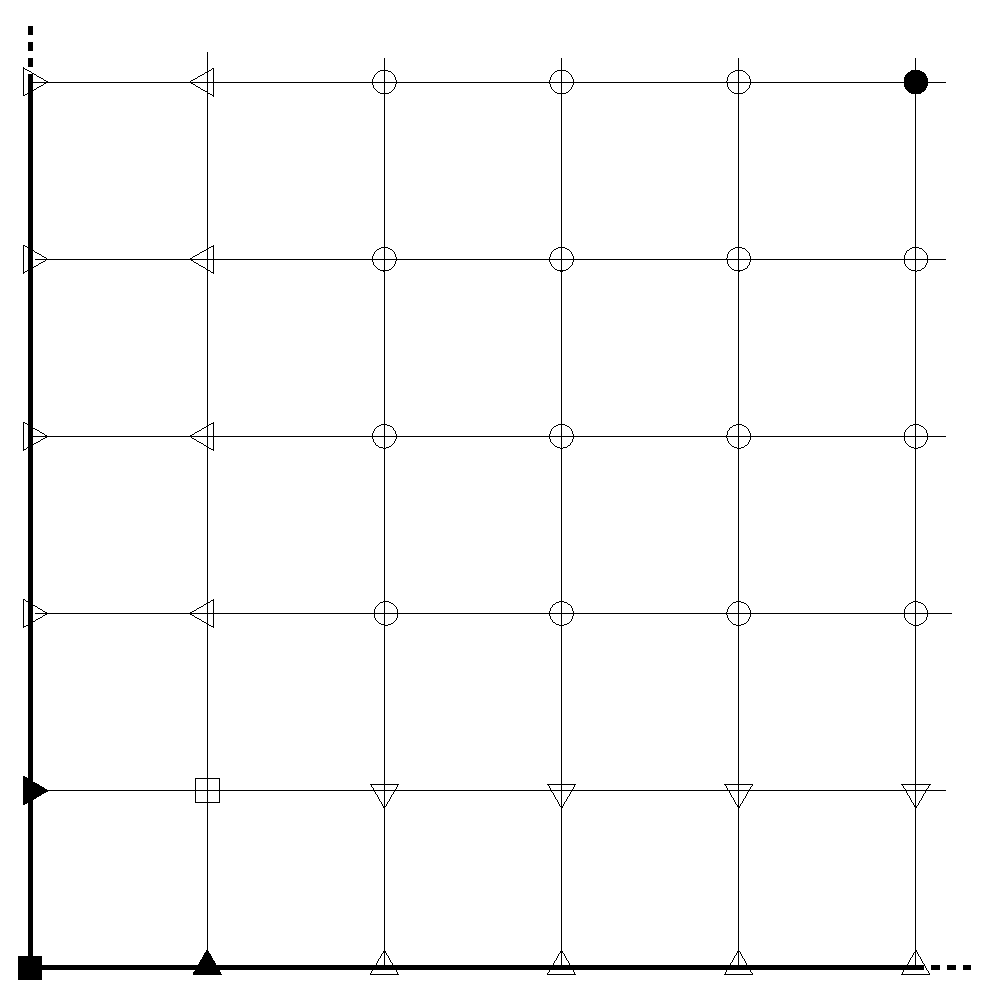
\includegraphics{BottomLeftCornerMesh.eps}}
\caption{Bottom--left corner of the mesh for second cross--derivative
evaluation.  Points requiring special treatment are indicated.}
\end{center}
\label{FigBOTTOMLEFT}
\end{figure}

\noindent
The mesh in the vicinity of a bottom--right non-periodic boundary corner
is shown in Figure 4.  The point at the top right indicated
by a filled circle is the closest point to the corner at which the full
10th--order centred cross--derivative scheme can be applied.
Close to non-periodic boundaries there are five special cases as
indicated in the Figure:
\begin{enumerate}
\item{For a corner point (filled square), a doubly
one--sided fourth order scheme is used which evaluates the first derivative
of the first derivative by combining two instances of
(\ref{FIRSTDERIVONESIDE}), one for each direction.}
\item{For a point on the boundary adjacent to a
corner (filled triangles), a mixed one--sided/skewed fourth--order scheme
is used combining instances of (\ref{FIRSTDERIVSKEW}) and
 (\ref{FIRSTDERIVONESIDE});}
\item{For an interior point located one point away from a corner in both
directions (open square), a doubly--skewed fourth--order scheme
is used which combines two instances of (\ref{FIRSTDERIVSKEW});}
\item{For an interior point located one point away from the boundary in
one direction but two or more points away from the boundary in the other
direction (open inverted and left--facing triangles), a mixed skewed/standard
fourth order scheme is used combining
instances of (\ref{FIRSTDERIV}) and (\ref{FIRSTDERIVSKEW});}
\item{For a boundary point located two or more points away from the boundary
in the other direction (open upright and right--facing triangles), a mixed
one--sided/standard fourth order scheme is used
which combines instances of (\ref{FIRSTDERIV}) and (\ref{FIRSTDERIVONESIDE}).}
\end{enumerate}
In all of the special cases, the appropriate combined differencing scheme is
applied to boundaries on all sides after suitable coordinate reflections.

\subsection{Mesh Stretching}
All derivatives are evaluated on a uniform mesh for best accuracy and
computational efficiency.  In some circumstances it is helpful to use a
non--uniform mesh, for example close to walls when extra mesh resolution is
needed in the wall--normal direction, or in the far field when mesh
resolution can be reduced without compromising the solution.  Mesh
stretching can be achieved by means of the one--dimensional coordinate
transformation
\begin{equation}
\frac{\partial f}{\partial \hat{x}} = 
\frac{\partial f}{\partial x}\frac{dx}{d\hat{x}}
\end{equation}
where $x$ is the relevant one--dimensional coordinate of the uniform
reference mesh and $\hat{x}$ is the transformed coordinate of the
required stretched mesh.  By specifying a suitable stretching function
$\hat{x}(x)$ analytically, it is possible to compute the derivatives on the
stretched mesh from those on the uniform mesh without incurring any
additional numerical error.  Second derivatives are evaluated using
\begin{equation}
\frac{\partial^{2} f}{\partial \hat{x}^{2}} = 
\frac{\partial^{2} f}{\partial x^{2}}
\left(\frac{dx}{d\hat{x}}\right)^{2} +
\frac{\partial f}{\partial x}\frac{d^{2}x}{d\hat{x}^{2}}
\end{equation}
while second cross--derivatives are evaluated using
\begin{equation}
\frac{\partial^{2} f}{\partial \hat{x}\partial y} = 
\frac{\partial^{2} f}{\partial x\partial y}\frac{dx}{d\hat{x}}
\end{equation}
An example of a suitable stretching function for use near a wall located
at the plane denoted by $x = 0$ is given by the hyperbolic tangent
mapping
\begin{equation}
\frac{d\hat{x}}{dx} = A\tanh{\left(ax + b\right)}
\end{equation}
where $a$ and $b$ are constant parameters chosen to give the desired stretching
rate and near--wall limiting behaviour respectively.  The normalising
constant $A$ can be found (for example) by matching the stretched domain to
the required global domain size.  For the case of a channel flow bounded by
walls at $x = 0$ and $x = L_{x}$, this type of mapping may be generalised in a
straightforward manner using
\begin{equation}
\frac{d\hat{x}}{dx} = A\left\{\tanh{\left(ax + b\right)}
-\tanh{\left(a(x-L_{x}) - b\right)}\right\}.
\end{equation}

\subsection{Parallel Domain Decomposition}
Parallel computation is facilitated using a simple domain decomposition
approach.  The global computational domain is decomposed into cuboidal
sub--domains which are each assigned to a CPU core.  The total
number of cores required is $P = P_{x}P_{y}P_{z}$ where $P_{x}$, $P_{y}$ and
$P_{z}$ are the numbers of cores assigned to the $x$, $y$ and $z$ directions
respectively.  The cores are ranked from $p=0$ to $p=P-1$, and are also
given Cartesian indices $(p_{x},p_{y},p_{z})$ ranging in $x-y-z$
order from $(1,1,1)$ to $(P_{x},P_{x}.P_{z})$.  Hence
\begin{equation}
p = (p_{x}-1) + (p_{y}-1)P_{x} + (p_{z}-1)P_{x}P_{y}
\end{equation}

\begin{figure}[htbp]
\begin{center}
\resizebox{100mm}{!}{\includegraphics{ParallelDomain.eps}}
\caption{Example of parallel domain decomposition.}
\end{center}
\end{figure}

The domain decomposition is carried out by dividing the number of mesh points
on each side of the global domain by the number of cores assigned to that
direction.  Hence the number of points allocated to the core with rank $p$
is given by $(n_{x}^{(p)},n_{y}^{(p)},n_{z}^{(p)})$ where 
$n_{x}^{(p)}=N_{x}/P_{x}$ and similarly for the $y$ and $z$ directions.
Load--balancing is achieved by ensuring that the same number of mesh
points is allocated to each sub--domain.  Where this is not possible,
for example due to $N_{x}$ not being divisible by $P_{x}$, an integer
division is carried out in each direction and the remainder is allocated to
the first--indexed core in that direction.  Figure 5 shows an example of a
domain decomposition with $P_{x}=4$, $P_{y}=2$, $P_{z}=4$ and equal
sub--domains.  Communication between adjacent sub--domains is done using
a layer of halo cells on the surface of each sub--domain.  Since the interior
tenth--order differencing stencil requires five points on each side of the
central point (see Figure 2), the halo layer is five points thick.  For the
scalar quantities, a halo layer is required only on each face of each
sub--domain.  For the velocity components, the need to evaluate second
cross--derivatives means that the halo layer must include the edges and
corners also.   

\begin{figure}[htbp]
\begin{center}
\resizebox{100mm}{!}{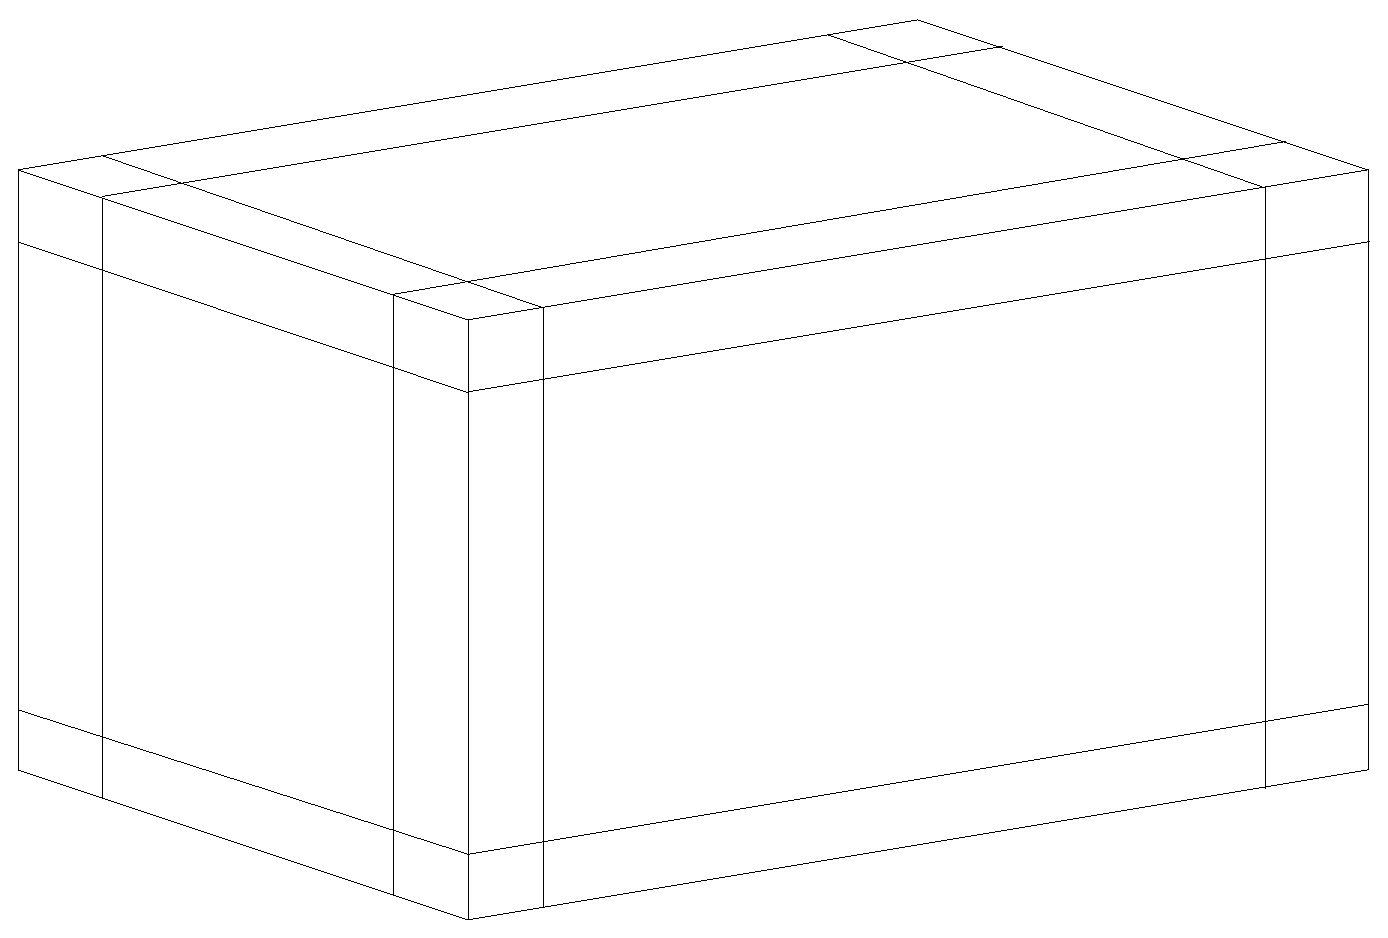
\includegraphics{ParallelHalos.eps}}
\caption{Full halo layer on the surface of a parallel sub--domain.}
\end{center}
\end{figure}

For a sub--domain of size $n_{x}n_{y}n_{z}$ and a halo layer thickness
$h$, the number of points in the augmented sub--domain illustrated in
Figure 6 is given by
\begin{equation}
(n_{x}+2h)(n_{y}+2h)(n_{z}+2h) = n_{x}n_{y}n_{z}
+ 2h\left(n_{x}n_{y} +n_{x}n_{z} + n_{y}n_{z}\right)
+ 4h^{2}\left(n_{x}+n_{y}+n_{z}\right) + 8h^{3}
\end{equation}
The terms on the right--hand side correspond to the number of points in
the original sub--domain, the number of points in the halos attached to
each face of the original sub--domain, the number of points in the halo
strips along each edge, and finally the number of points in the eight
corners of the halo.  The fractional increase in the number of points
compared to the original sub--domein is given by the expression
\begin{equation}
\frac{(n_{x}+2h)(n_{y}+2h)(n_{z}+2h)}{n_{x}n_{y}n_{z}} - 1 =
  \frac{2h}{n_{x}} + \frac{2h}{n_{y}} + \frac{2h}{n_{z}}
+ \frac{4h^{2}}{n_{x}n_{y}}
+ \frac{4h^{2}}{n_{x}n_{z}}
+ \frac{4h^{2}}{n_{y}n_{z}}
+ \frac{8h^{3}}{n_{x}n_{y}n_{z}}
\end{equation}
Since in general $h<<n_{x,y,z}$, it is clear that the computational
overhead associated with the halo is dominated by the first three terms
on the right--hand side.  The lowest overhead is obtained when $n_{x} =
n_{y} = n_{z} = n$, i.e. when the surface--to--volume ratio of the
sub--domain is at a minimum.  Parallel communication is implemented using
MPI.


\subsection{Time Stepping}
Time advancement of the solution is carried out using a low--storage
explicit Runge--Kutta method with adaptive time step control
\cite{KennedyCarpenterLewis}.  The governing
equations (\ref{CONTINUITY})--(\ref{MASSFRAC}) are written as
\begin{equation}
\frac{\partial {\mathbf U}}{\partial t}
= {\mathbf R}({\mathbf U},t)
\label{GovEqConservRK}
\end{equation}
where ${\mathbf U}$ is the vector of conserved variables given by
${\mathbf U} = \{\rho, \rho u, \rho v, \rho w, \rho E, \rho Y_{\alpha}\}^{T}$
and ${\mathbf R}$ is the right--hand side vector containing all other terms
in the equations.  Clearly ${\mathbf R}$ depends on ${\mathbf U}$ and
may also depend explicitly on time, for example through source terms or
boundary conditions.  The general $s$--stage explicit Runge--Kutta
scheme may be stated as:
\begin{eqnarray}
{\mathbf U}^{(i)} & = & {\mathbf U}^{(n)}
                  + \delta t\sum_{j=1}^{i-1}a_{ij}{\mathbf R}^{(j)} \nonumber\\
{\mathbf U}^{(n+1)} & = & {\mathbf U}^{(n)}
                    + \delta t\sum_{j=1}^{s}b_{j}{\mathbf R}^{(j)} \nonumber\\
t^{(i)} & = &  t^{(n)} + c_{i}\delta t \nonumber \\
\hat{{\mathbf U}}^{(n+1)} & = & {\mathbf U}^{(n)}
               + \delta t\sum_{j=1}^{s}\hat{b}_{j}{\mathbf R}^{(j)}
\end{eqnarray}
where ${\mathbf R}^{(i)} = {\mathbf R}({\mathbf U}^{(i)},t^{(i)})$ and
the last line denotes the lower--order embedded scheme used to provide
error estimates for the adaptive time--step controller.  Memory
requirements are minimised by using a two--register scheme which
requires the storage of only ${\mathbf U}^{(i)}$ and ${\mathbf R}^{(i)}$ at
each stage.  In practice it is necessary also to store $\hat{\mathbf U}^{(i)}$
and to provide some temporary storage for intermediate data required in
the evaluation of ${\mathbf R}^{(i)}$.  The order of the scheme is
determined by constraints on the coefficients $a_{ij}$, $b_{i}$ and $c_{i}$
while the order of the embedded scheme is determined using the coefficients
$\hat{b}_{i}$ in place of $b_{i}$.  Several schemes were assessed, and a
five--stage
fourth--order two--register method with a third--order embedded scheme
was chosen.  This scheme is denoted RK4(3)5[2R+]C in the classification of
Kennedy at al. \cite{KennedyCarpenterLewis} and its Butcher array is
given in Table 4.

\begin{table}[htbp]
\begin{center}
\begin{tabular}{c|ccccc}
0 &  &  &  &  &  \\
$c_{2}$ & $a_{21}$ &  &  &  &  \\
$c_{3}$ & $b_{1}$ & $a_{32}$  &  &  &  \\
$c_{4}$ & $b_{1}$ & $b_{2}$ & $a_{43}$  &  &  \\
$c_{5}$ & $b_{1}$ & $b_{2}$ & $b_{3}$ &  $a_{54}$  &  \\ \hline
        & $b_{1}$ & $b_{2}$ & $b_{3}$ &  $b_{4}$   &  $b_{5}$
\end{tabular}
\caption{Butcher array for the RK4(3)5[2R+]C explicit Runge--Kutta method.}
\end{center}
\end{table}

The numerical values of the coefficients are given in Table 5.

\begin{table}[htbp]
\begin{center}
\begin{tabular}{|c|c|c|c|c|c|} \hline
  &  &  &  &  & \\
$a_{21}$ & $\frac{970286171893}{4311952581923}$ &
$b_{1}$  & $\frac{1153189308089}{22510343858157}$ &
$\hat{b}_{1}$ & $\frac{1016888040809}{7410784769900}$ \\
  &  &  &  &  & \\
$a_{32}$ & $\frac{6584761158862}{12103376702013}$ &
$b_{2}$  & $\frac{1772645290293}{4653164025191}$ & 
$\hat{b}_{2}$ & $\frac{11231460423587}{58533540763752}$ \\
  &  &  &  &  & \\
$a_{43}$ & $\frac{2251764453980}{15575788980749}$ &
$b_{3}$ & $\frac{-1672844663538}{4480602732383}$ &
$\hat{b}_{3}$ & $\frac{-1563879915014}{6823010717585}$ \\
  &  &  &  &  & \\
$a_{54}$ & $\frac{26877169314380}{34165994151039}$ &
$b_{4}$ & $\frac{2114624349019}{3568978502595}$ &
$\hat{b}_{4}$ & $\frac{606302364029}{971179775848}$ \\
  &  &  &  &  & \\
        &   &
$b_{5}$ & $\frac{5198255086312}{14908931495163}$ &
$\hat{b}_{5}$ & $\frac{1097981568119}{3980877426909}$ \\
  &  &  &  &  & \\ \hline
\end{tabular}
\caption{Coefficients for the RK4(3)5[2R+]C explicit Runge--Kutta method.}
\end{center}
\end{table}

The two--register Runge--Kutta method is implemented as a sequence of
sub--steps.  At the beginning of a new time step, the time is set to
$t^{(1)}=t^{(n)}$.  The first register contains the initial stage value
${\mathbf S}^{(1)} = {\mathbf U}^{(n)}$ while the second register contains
the initial solution value ${\mathbf U}^{(1)} = {\mathbf U}^{(n)}$. 
The error accumulator ${\mathbf E}^{(1)}$ is set initially to zero.  In
each sub--step $j$, the right--hand side function ${\mathbf R}^{(j)}$ is
evaluated using the current time and the current solution value
${\mathbf U}^{(j)}$.  The new value of ${\mathbf R}^{(j)}$ is stored in
Register 2, overwriting ${\mathbf U}^{(j)}$.  Then new values of both 
${\mathbf S}$ and ${\mathbf U}$ are formed by linear combinations of
${\mathbf S}^{(j)}$ and ${\mathbf R^{(j)}}$ and are stored in place.
At the final step, only ${\mathbf S}$ is updated and becomes the new
solution at time $t^{(n+1)}$.  The error accumulator is updated at each
sub--step as new values of ${\mathbf R}$ become available.

\begin{table}[htbp]
\begin{center}
\begin{tabular}{|c||c|c||c|} \hline
Time & Register 1 & Register 2 & Error accumulator \\ \hline
$t^{(1)}$ & ${\mathbf S}^{(1)}$ & ${\mathbf U}^{(1)}$ &
 ${\mathbf E}^{(1)}$ \\ \hline
 & ${\mathbf S}^{(1)}$ &
 ${\mathbf R}^{(1)}\left({\mathbf U}^{(1)},t^{(1)}\right)$ &
 ${\mathbf E}^{(1)}$ \\ \hline
 &
 ${\mathbf S}^{(2)} = {\mathbf S}^{(1)} + b_{1} \delta t \mathbf R^{(1)}$ &
 ${\mathbf U}^{(2)} = {\mathbf S}^{(1)} + a_{21}\delta t \mathbf R^{(1)}$ &
 ${\mathbf E}^{(2)} = {\mathbf E}^{(1)}
                    + \left(b_{1}-\hat{b}_{1}\right)\delta t \mathbf R^{(1)}$
 \\ \hline
 $t^{(2)} = t^{(1)} + c_{2}\delta t$ &
 ${\mathbf S}^{(2)}$ &
 ${\mathbf R}^{(2)}\left({\mathbf U}^{(2)},t^{(2)}\right)$ &
 ${\mathbf E}^{(2)}$ \\ \hline
 &
 ${\mathbf S}^{(3)} = {\mathbf S}^{(2)} + b_{2} \delta t \mathbf R^{(2)}$ &
 ${\mathbf U}^{(3)} = {\mathbf S}^{(2)} + a_{32}\delta t \mathbf R^{(2)}$ &
 ${\mathbf E}^{(3)} = {\mathbf E}^{(2)}
                    + \left(b_{2}-\hat{b}_{2}\right)\delta t \mathbf R^{(2)}$
 \\ \hline
 \vdots & \vdots & \vdots & \vdots \\ \hline
 $t^{(5)} = t^{(1)} + c_{5}\delta t$ &
 ${\mathbf S}^{(5)}$ &
 ${\mathbf R}^{(5)}\left({\mathbf U}^{(5)},t^{(5)}\right)$ &
 ${\mathbf E}^{(5)}$ \\ \hline
 &
 ${\mathbf S}^{(6)} = {\mathbf S}^{(5)} + b_{5} \delta t \mathbf R^{(5)}$ &
 ${\mathbf U}^{(5)} $ &
 ${\mathbf E}^{(6)} = {\mathbf E}^{(5)}
                    + \left(b_{5}-\hat{b}_{5}\right)\delta t \mathbf R^{(5)}$
 \\ \hline
 $t^{(n+1)} = t^{(5)}$ &
 ${\mathbf U}^{(n+1)} = {\mathbf S}^{(6)}$ &
 ${\mathbf U}^{(n+1)}$ &
 ${\mathbf E}^{(n+1)} = {\mathbf E}^{(6)}$
 \\ \hline
\end{tabular}
\caption{Sequence of sub--steps for Runge--Kutta implementation.}
\end{center}
\end{table}

\noindent
The time step is set adaptively using a PID--based controller
\cite{KennedyCarpenterLewis}.  The new time step $\delta t^{(n+1)}$ is given
by
\begin{equation}
\delta t^{(n+1)}=\kappa\delta t^{(n)}
\left(\frac{\varepsilon}{||E^{(n+1)}||_{\infty}}\right)^{\alpha}
\left(\frac{||E^{(n)}||_{\infty}}{\varepsilon}\right)^{\beta}
\left(\frac{\varepsilon}{||E^{(n-1)}||_{\infty}}\right)^{\gamma}
\end{equation}
where $E$ is an error estimate obtained by finding the maximum of the
normalised elements of ${\mathbf E}$, $\varepsilon$ is a pre--set error
tolerance, $\kappa$ is a safety factor and $\alpha$, $\beta$ and
$\gamma$ are the parameters of the controller.  The controller requires
some tuning for optimal performance, but good results have been obtained
with $\varepsilon = 1.0\times 10^{-3}$, $\kappa=0.9$, $\alpha = 0.49/p$,
$\beta = 0.34/p$ and $\gamma = 0.1/p$ where $p=3$ is the order of the
embedded method.   

\subsection{Initial Turbulent Field}
\label{ParFFT}
A three--dimensional parallel inverse Fourier transform is implemented
as part of the turbulence initialisation procedure.  The
three--dimensional transform algorithm is based on a superposition of
three separate one--dimensional transforms.  During each
one--dimensional transform, all of the data along each
single line of the global computational mesh (i.e. a single ``pencil'' of data)
is gathered onto the lowest--ranked processor on that line.  A one--dimensonal
inverse Fourier transform is carried out on that processor, and the pencil of
transformed data is scattered back to its original
locations.  Multiple pencils may be handled at the same time, in
order to reduce parallel communication overheads.  The one--dimensional
transform is based on the prime--factor fast Fourier transform algorithm
\cite{Temperton} as implemented in a locally--developed FFT library
\cite{FFTlib}.  In principle the FFT algorithm
will handle any length of transform data, although optimal performance is
obtained for lengths which are powers of two or three.  The final
one--dimensional transform procedure includes a step which imposes the symmetry
conditions necessary to ensure that the physical--space velocity field
is purely real.   Further details are given in a separate report
\cite{Starturb}.

\newpage
\section{Running the Code}
Setting up a DNS run using {\tt SENGA2} requires several steps.  First
the size of the computational domain and the size parameters for the
thermochemical problem must be set by editing the {\tt COMMON} blocks.  Then
the control parameters for the run must be set using the control data
file, and the relevant chemical, molecular transport and thermal radiation data
must be provided using the relevant data files.

\subsection{Common Data}
The common data for {\tt SENGA2} is contained in the {\tt COMMON} block file
{\tt com\_senga2.h}.  This file must be edited in order to set the global
and local sizes of the computational domain, the number of processors and
the size of the parallel transfer array.

The section {\tt PHYDIM} is the first section of the file {\tt com\_senga2.h}
and an example is shown below:
\begin{verbatim}
C     PHYDIM-------------------------------------------------------------------

C     PHYSICAL DIMENSIONS OF ARRAYS
C     -----------------------------
C     NOTE: ALL ARRAY SIZES MUST BE CONSISTENT
C     NXSIZE MUST BE >= NXGLBL/NXPROC
C     NYSIZE MUST BE >= NYGLBL/NYPROC
C     NZSIZE MUST BE >= NZGLBL/NZPROC
C     WITH AN EXTRA ALLOWANCE FOR ANY REMAINDER
C     
C     GLOBAL GRID SIZE
      INTEGER NXGLBL,NYGLBL,NZGLBL
      PARAMETER(NXGLBL=64, NYGLBL=64, NZGLBL=64)
      INTEGER NGZMAX
C     SET NGZMAX=MAX(NXGLBL,NYGLBL,NZGLBL)
      PARAMETER(NGZMAX=NXGLBL)

C     NUMBER OF PROCESSORS
      INTEGER NXPROC,NYPROC,NZPROC
      PARAMETER(NXPROC=2, NYPROC=2, NZPROC=2)
      INTEGER NPRMAX
C     SET NPRMAX=MAX(NXPROC,NYPROC,NZPROC)
      PARAMETER(NPRMAX=NYPROC)

C     LOCAL GRID SIZE
      INTEGER NXSIZE,NYSIZE,NZSIZE
      PARAMETER(NXSIZE=32, NYSIZE=32, NZSIZE=32)
      INTEGER NSZMAX
C     SET NSZMAX=MAX(NXSIZE,NYSIZE,NZSIZE)
      PARAMETER(NSZMAX=NZSIZE)

C     SIZE OF HALO
      INTEGER NHALOX,NHALOY,NHALOZ
      PARAMETER(NHALOX=5,NHALOY=5,NHALOZ=5)

C     SIZE OF PARALLEL TRANSFER ARRAY
C     NPARAY MUST BE >= MAX(NHALOX,NHALOY,NHALOZ)
C                            *MAX((NXSIZE+2*NHALOX)*(NYSIZE+2*NHALOY),
C                                 (NXSIZE+2*NHALOX)*(NZSIZE+2*NHALOZ),
C                                 (NYSIZE+2*NHALOY)*(NZSIZE+2*NHALOZ))
C     AND ALSO LARGE ENOUGH FOR PARALLEL BROADCAST OF CHEMICAL DATA
C     AND ALSO LARGE ENOUGH FOR PARALLEL TRANSFER OF INITIAL TURBULENCE DATA
      INTEGER NPARAY
      PARAMETER(NPARAY=8820)
      .
      .
      .
C     PHYDIM-------------------------------------------------------------------
\end{verbatim}
Here, the parameters {\tt NXGLBL}, {\tt NYGLBL} and {\tt NZGLBL} must be
set to define the global size of the computational domain in terms of
the number of grid points required in the $x$, $y$ and $z$
directions respectively.  These must be the exact global domain sizes required.
The parameter {\tt NGZMAX} must be set equal to the largest of the
three global domain sizes.

It is assumed that the problem will be decomposed
over a topologically cubical array of processors.  The parameters {\tt NXPROC},
{\tt NYPROC} and {\tt NZPROC} must be set to define the number of processors to
be used in each direction, and {\tt NPRMAX} must be set equal to the largest of
these.

The parameters {\tt NXSIZE}, {\tt NYSIZE} and {\tt NZSIZE} must be set to
define the maximum size of the computational
domain on each processor.  The global domain is decomposed by {\tt SENGA2}
as evenly as possible between the processors in each direction: thus
{\tt NXSIZE} must be set to a value greater than or equal to 
{\tt NXGLBL/NXPROC}.  If {\tt NXGLBL} is not exactly divisible by
{\tt NXPROC} then the remainder is evenly distributed between the
highest-ranked processors in the $x$-direction.  In that case {\tt
NXSIZE} must be set greater than or equal to {\tt 1 + NXGLBL div NXPROC}.
Clearly the same procedure must be followed also for the other two directions
in setting {\tt NYSIZE} and {\tt NZSIZE}.  Then {\tt NSZMAX} must be set
equal to the largest of the three local domain sizes.

The parameters {\tt NHALOX}, {\tt NHALOY} and {\tt NHALOZ}  must be set to
define the width of the halo
layer of the computational grid that is passed between adjacent
processors in each direction, and the value set must match the
corresponding interior spatial
differencing scheme in use.  These parameters must be set even if the
problem uses only a single processor.  The default values for the standard 10th
order interior differencing scheme are {\tt NHALOX=NHALOY=NHALOZ=5}.

The parameter {\tt NPARAY} controls the the size of the parallel transfer
array.  The value of
{\tt NPARAY} must be set greater than or equal to the maximum halo size
required in each direction, i.e. the maximum of
{\tt NHALOX}, {\tt NHALOY}, {\tt NHALOZ}, multiplied by the maximum of\\
{\tt (NXSIZE+2*NHALOX)*(NYSIZE+2*NHALOY)} for the $z$-direction,\\
{\tt (NXSIZE+2*NHALOX)*(NZSIZE+2*NHALOZ)} for the $y$-direction, and\\
{\tt (NYSIZE+2*NHALOY)*(NZSIZE+2*NHALOZ)} for the $x$-direction.\\
The value of {\tt NPARAY} must be greater than or equal to the
maximum required to broadcast the control data and the chemical data
during initialisation of the code.  This is checked automatically during
start-up.\\

If an initial turbulent field is required, it may be useful to edit the
the section {\tt IFTURB} of the file {\tt com\_senga2.h} which is shown
below:
\begin{verbatim}
C     IFTURB-------------------------------------------------------------------

C     DATA FOR INITIAL TURBULENCE FIELD

C     NUMBER OF PENCILS
      INTEGER NPENMX
      PARAMETER(NPENMX=16)

      DOUBLE PRECISION FFTROW(2*NGZMAX,3,NPENMX),
     +                 FTPART(2*NSZMAX,3,NPENMX),
     +                 FFTINX(2*NGZMAX)

      COMMON/IFTURB/FFTROW,FTPART,FFTINX

C     IFTURB-------------------------------------------------------------------
\end{verbatim}
The parameter {\tt NPENMX} controls the number of FFT pencils (i.e. lines of
one-dimensional transform data) which are transferred between processors
in a single batch.  The minimum value is {\tt NPENMX=1}, and any larger
value provides a gain in the speed of inter-processor communication during the
generation of the initial turbulent field at the cost of the memory
required to store the transform data.\\

The section {\tt CHEMIC} of the file {\tt com\_senga2.h} contains the
thermochemical data and is shown below:
\begin{verbatim}
C     CHEMIC-------------------------------------------------------------------

C     PARAMETERS
C     ==========
C     MAX NO OF SPECIES, NO OF STEPS
      INTEGER NSPCMX,NSTPMX
      PARAMETER(NSPCMX=1, NSTPMX=1)

C     THERMODYNAMIC DATA
C     MAX NO OF TEMPERATURE INTERVALS, THERMO POLYNOMIAL COEFFICIENTS
      INTEGER NTINMX,NCOFMX
      PARAMETER(NTINMX=2, NCOFMX=7)
C     MAX NO OF TEMPERATURE COEFFICIENTS, DITTO MINUS ONE
      INTEGER NCTMAX,NCTMM1
      PARAMETER(NCTMAX=5, NCTMM1=NCTMAX-1)

C     TEMPERATURE INTERVAL INDEXING
C     NTBASE = NUMBER BASE FOR INDEXING:
C     MUST BE A POWER OF TWO >= MAX NO OF TEMPERATURE INTERVALS PER SPECIES
C     NSPIMX = MAX NO OF SPECIES STORED PER SINGLE (32-BIT) SIGNED INTEGER:
C     MUST BE SET EQUAL TO 31 DIV LOG2(NTBASE)
C     NINTMX = NO OF INTEGERS REQUIRED PER SPATIAL POINT:
C     MUST BE SET EQUAL TO (1 + NSPCMX DIV NSPIMX)
      INTEGER NTBASE,NSPIMX,NINTMX
      PARAMETER(NTBASE=4, NSPIMX=15, NINTMX=1)

C     CHEMICAL RATE DATA
C     MAX NO OF THIRD BODIES
      INTEGER NBDYMX
      PARAMETER(NBDYMX=10)
C     MAX SIZE OF STEP SPECIES-LIST, STEP REACTANT-LIST
      INTEGER NSSMAX,NRSMAX
      PARAMETER(NSSMAX=10, NRSMAX=10)
C     MAX NO OF LINDEMANN STEPS
      INTEGER NLLMAX
      PARAMETER(NLLMAX=10)

C     TRANSPORT COEFFICIENTS
      DOUBLE PRECISION ALAMDC,RLAMDA,TLAMDA
      PARAMETER(ALAMDC=2.58D-5, RLAMDA=7.0D-1, TLAMDA=2.98D2)
      DOUBLE PRECISION PRANTL
      PARAMETER(PRANTL=7.0D-1)
      .
      .
\end{verbatim}
The parameter {\tt NSPCMX} sets the maximum number of chemical species
while {\tt NSTPMX} sets the maximum number of steps in the reaction
mechanism.  The minimum value for each is 1, and it is expected that
both of these parameters will be set equal to the corresponding values
in the chemical data file (see below).  This is checked automatically
during startup.  A legitimate exception 
occurs for non-reacting flow, when {\tt NSTPMX=1} and the number of reaction
steps is actually equal to zero. 

The parameters {\tt NTINMX}, {\tt NCOFMX} and {\tt NCTMAX} control the
maximum sizes required to store the thermodynamic data for each species
expressed in polynomial form (eq. \ref{CPPOLY}).  The parameter {\tt NTINMX}
sets the maximum
number of temperature intervals required for any species while {\tt NCOFMX}
sets the maximum number of coefficients required in each interval.  The
parameter {\tt NCTMAX} sets the maximum number of
coefficients required in the polynomial for temperature (eq. \ref{TEMPERPOLY}).

The index of the current temperature interval for each species is stored
in {\tt SENGA2} in order to avoid the need for repeated searching and a
bit-wise compression algorithm is used to conserve memory.  The parameter {\tt
NTBASE} defines the number base for the compression algorithm and 
must be set to an integer value that is a power of two and is
greater than or equal to the maximum number of temperature intervals per
species {\tt NTINMX}.  The parameter {\tt NSPIMX} defines the maximum
number of species temperature indices that can be stored in a single
32-bit signed integer using the number base {\tt NTBASE} and its value
must be set equal to
{\tt NSPIMX = 31 DIV LOG2(NTBASE)}.  The parameter {\tt NINTMX} defines
the number of integers required per spatial point.  Clearly the product
{\tt NSPIMX*NINTMX} must be greater than or equal to the maximum number of
species {\tt NSPCMX}.

Size parameters for the chemical rate data must also be set.  The parameter
{\tt NBDYMX} must be set greater than or equal to the maximum number of
distinct third bodies.  The parameter {\tt NSSMAX} must be set
greater than or equal to the maximum number of species involved in any
single reaction step.  Similarly, the parameter {\tt NRSMAX} must be set
greater than or equal to the maximum number of reactant species involved in
any single reaction step.  The parameter {\tt NLLMAX} must be set
greater than or equal to the maximum number of reaction steps requiring
Lindemann rate data. Note that these parameters
are used only to set array sizes, and actual values
for these quantities are set in the chemical data file. 

The values of the parameters used to evaluate the transport
coefficients according to (eq. \ref{TRANSRELAT}) are set.  Clearly {\tt
ALAMDA} and {\tt RLAMDA} represent the multiplicative coefficient and
temperature exponent respectively while {\tt TLAMDA} is the reference
temperature.  The mixture Prandtl number in (eq. \ref{VISCRELAT}) is set
using the parameter {\tt PRANTL}.

When the editing of {\tt com\_senga2.h} is complete, all {\tt FORTRAN} source
files for {\tt SENGA2} must be recompiled in order to incorporate the
changes into the code.

\subsection{Control Data}
The control data file {\tt cont.dat} must be edited to set up
the control parameters for the run.  The file format is as shown:
\begin{verbatim}
*************************************************
**                                             **
**       SENGA2: Run control data file         **
**                                             **
*************************************************

Global domain size (x,y,z) in metres
 1.0D-2   1.0D-2   1.0D-2

Global domain size (nx,ny,nz)
 64    64     64

No. of processors (x,y,z)
 2      2      2

Time step; start step, no of steps, step switch (0=fixed, 1=adaptive)
 1.0D-12    1   1000   1

Intervals between dumps, reports, statistics
 500    1     500

Cold start switch (0=cold start, 1=restart)
 0

Initial turbulence generator
switch (0=off, 1=new, 2=inlet); random seed; spectrum parameters
 1      -1      8.51064D0   5.0D0  0.0D0  0.0D0

Flame generator switch (0=off, 1=on) 
 0

Default initial conditions
pressure, temperature, velocity components u,v,w
 1.0D5   3.0D2   3.9D-1  0.0D0  0.0D0
mass fractions
 1
 1    1.0D0

Global boundary condition types
one per line: x-left; x-right; y-left; y-right; z-left; z-right
(1=periodic; 1a=inlet; 2b=outlet; 3c=wall; a,b,c denotes BC subtype)
(four integer and four real parameters allowed for each)
13    1    0    0   0   3.9D-1    0.0D0    0.0D0     0.0D0
21    0    0    0   0   1.0D5     2.87D0   1.0D-3    0.0D0
1     0    0    0   0   0.0D0     0.0D0    0.0D0     0.0D0
1     0    0    0   0   0.0D0     0.0D0    0.0D0     0.0D0
1     0    0    0   0   0.0D0     0.0D0    0.0D0     0.0D0
1     0    0    0   0   0.0D0     0.0D0    0.0D0     0.0D0

Molecular transport control data
switches: mix.av, mol.mass, pressure, Soret, Dufour; mol.mass limit
0     1    1    1   1   5.0D0

Radiation control data
switch, reference temperature
1     3.0D2

End of file
\end{verbatim}
The first five lines are treated as a header and are read but ignored by
the {\tt SENGA2} code.  The various data items are then listed in groups,
and the
format of the control file is fixed to the extent that the number of lines
in each group and the number of data items per line must be preserved.\\

\noindent
The global size of the domain in the $x$, $y$ and $z$ directions
must be specified in metres, together with the global size of the domain in
terms of the number of grid points in each direction and the number of
processors in each direction.  The values for global grid size and number of
processors must be set to match those already specified in {\tt com\_senga2.h},
and this is checked by {\tt SENGA2} during initialisation.  Note that the
processors are ranked from 0 such that the rank index increases by counting
along the $x$, $y$ and $z$ directions in that order.\\

\noindent
The initial time step must be set (in seconds), together with the index of
the first
time step and the required number of time steps for the run.  A switch
must be set to control whether a fixed time step (switch={\tt 0}) or adaptive
time-stepping (switch={\tt 1}) is required.
The number of time steps between dumps must be set.  A restart file is
written for each processor at the start of a run, and a further restart
file is dumped for each processor after the specified number of time steps.
Throughout the remainder of the run.  In order to help guard against loss of
data, two restart files are kept for each
processor and the older file of the two is overwritten at each dump.
The restart file names conform to the pattern
{\tt dmpiXXXY.dat} where {tt XXX} is the rank
index of the corresponding processor (starting from {\tt 000}) and {\tt
Y} is the
restart file index which is either {\tt 0} or {\tt 1}.  The latest dump may be
contained in either restart file and alternates between the two.
The number of time steps between updates to the report file and the
statistics file must also be set.  A single report file
and a single statistics file are each created at the start of the run by the
lowest-ranked processor.  Each is updated after the specified number
of time steps.\\

\noindent
Initial conditions for the run must be set.  The cold start switch
must be set to {\tt 0} for a cold start, in which the run is initialised from
scratch using specified initial data.  Alternatively, the cold start
switch must be set to 1 for a restart, using data from a previous dump.
A restart file must exist for each processor, and the restart file names must
conform to the pattern {\tt dmpiXXXY.dat} where {tt XXX} is the rank
index of the corresponding processor and {\tt Y} is the restart file index.
It is expected that {\tt Y} will be set to {\tt 0} for a restart.\\

\noindent
The initial turbulence generator switch must be set to {\tt 0} if no initial
turbulent field is to be generated, or set to {\tt 1} if a fresh initial
turbulent field is to be generated.
If the switch is set to {\tt 1}
then the random seed must also be set in order to initialise the random
number generator.  If the (integer) value of the
random seed is set to be non-negative, the value set is
added to the rank of each processor in order to produce a different
random seed for each processor.  This ensures that there is no
repetition of the same random sequence on each processor.  Conversely,
if the value of the random
seed is set to be a negative integer, the value is used globally in order to
ensure
that the same global initial turbulent field is generated for a given global
grid size irrespective of the number of processors in use.
Up to four parameters may be set in order to control the initial turbulence
spectrum function defined in subroutine {\tt ESPECT} within {\tt SENGA2}.
The default spectrum function is the Batchelor--Townsend spectrum
\cite{BatchelorTownsend} which is described in section \ref{TURBINIT} and which
requires the use of only the first two parameters: these control the total
amount of turbulence kinetic energy and the wavenumber at which the
spectrum function has its peak.
If the initial turbulence generator switch is set to {\tt 2}, then a
previously--generated field of frozen inlet turbulence is copied into
the domain.  This facility exists to ensure continuity of the turbulent
field across the inlet boundary in cases where a turbulent inflow is
specified.\\

\noindent
The initial flame generator
switch must be set to {\tt 1} if an initial scalar field is to be specified,
or set to {\tt 0} if not.  This switch controls whether or not the
subroutine {\tt FLAMIN} is called within {\tt SENGA2}.  This subroutine is
designed to allow for the specification of an initial scalar field of
arbitrary complexity.\\

\noindent
Default initial conditions must be set for each
variable.  Pressure, temperature and the three velocity components must be
set using SI units.  The total number of species must be set
and must correspond to the
number of species specified in {\tt com\_senga2.h}.  This is checked by {\tt
SENGA2} during startup.  For each species an index number and a value
for its initial mass fraction must be set.  Each index number must correspond
to the species number specified in the chemical data file {\tt chem.dat}
as described below.  The
total of all mass fractions must be equal to
unity, and this is checked by {\tt SENGA2} during startup.\\

\noindent
Boundary condition types must be specified for the global domain.  This
is done using an indexing system, and up to four real and four integer
parameters may be set for each boundary condition subtype.\\[1mm]
Periodic boundary conditions are
specified using an index value of {\tt 1}.  Both of the corresponding periodic
faces of the domain must have this index value and this is checked
during startup.\\[1mm]
Inlet boundaries are specified using an index value of
{\tt 1a}, where {\tt a} denotes the inlet boundary condition subtype.
Three inlet boundary condition subtypes are implemented:\\[1mm] 
{\tt 11} Subsonic non-relecting laminar inflow \\
This condition requires no additional parameters to be set.\\[1mm]
{\tt 12} Subsonic reflecting turbulent inflow with specified temperature \\
By default the inlet temperature is set to the same value as specified
for the default initial temperature.\\[1mm]
{\tt 13} Subsonic reflecting turbulent inflow with specified density \\
By default the inlet density is set to the same value as the 
initial density as computed from the values specified for the default
initial pressure, temperature and species mass fractions.\\[2mm]
For inlet boundary condition subtypes {\tt 12} and {\tt 13}, the value of
the first integer parameter
determines the nature of the inlet velocity field.
A value of {\tt 1}
specifies a laminar inflow with constant velocity, whereupon the first real
parameter is taken to
specify the inflow velocity component normal to the boundary.
A value of {\tt 2} specifies a laminar inflow with velocity varying
sinusoidally in time, whereupon the first two real parameters specify the
amplitude and period of the oscillation.  A value of {\tt 3} specifies a
turbulent inflow.  In this case, the second integer parameter must be set
to {\tt 0} for a
cold start of the turbulent inlet velocity field, or to {\tt 1} for a restart.
The turbulent inflow velocity field is specified using Fourier
interpolation onto a scanning plane passing through a stored cubic box of
precomputed frozen turbulence, as described above.  
For a cold start, the first three real parameters must be set.  In
order, these specify the inlet mean velocity, the difference between the
scanning plane velocity and the inlet mean velocity, and the initial scanning
plane location as a distance (in metres) from the downstream end of the
stored box.  An input file is required for each processor.  The cold
start input filename has the form {\tt tcxlXXX.dat} where {\tt XXX} is the  
rank index of the corresponding processor.  The file has the same format
as a {\tt SENGA2} dump file, i.e a {\tt FORTRAN} unformatted file containing
all of the variables required for a full restart of the code.  For an
inlet cold start only the velocity field data is extracted from the file.
The intention is that the inlet velocity field would be generated from a
previous run of {\tt SENGA2} with appropriate initial conditions and 
possibly using periodic boundary conditions.  For a restart, the input
filename has the form {\tt tixlXXX.dat} where {\tt XXX} is the rank
index of the corresponding processor.  This file is generated by {\tt
SENGA2} during an inlet cold start and subsequently at the same time
as each scheduled dump.  It is a {\tt FORTRAN}
unformatted file containing the Fourier coefficients of the three
velocity components together with the current values of the scanning
plane location, the scanning velocity and the inlet mean velocity.\\

\noindent
Outlet boundaries are specified using an index of {\tt 2b},
where {\tt b} denotes the outlet boundary condition subtype.\\[1mm]
{\tt 21} Subsonic non--reflecting outflow \\
This condition requires three real parameters to be set.  In order,
these specify the pressure at infinity, the relaxation parameter and the
nominal boundary Mach number.\\

\noindent
Wall boundaries are specified using an index of {\tt 3c},
where {\tt c} denotes the wall boundary condition subtype.  The 
list of boundary condition types as implemented in the code is given
below:\\[1mm]
{\tt 31} Adiabatic no-slip wall \\
This condition requires no additional parameters to be set.\\[1mm]
{\tt 32} Isothermal no-slip wall \\
This condition requires a single real parameter to be set in order to
specify the wall temperature.\\

\noindent
The treatment of molecular transport must be specified.  There are five integer
switches.  The mixture--averaged switch must be set to {\tt 0} to select the
constant Lewis number treatment, or set to {\tt 1} to select mixture-averaged
transport.  If the constant Lewis number treatment is selected then the rest of
the molecular transport control data is ignored, the species Lewis numbers are
taken from the chemical data file and there is no need to provide a molecular
diffusion data file.  If mixture--averaged transport is selected then the
remaining molecular transport control data must be specified and a
molecular transport data file must be provided.

The molar mass switch must be set to {\tt 1} to activate
the molar mass gradient term in (\ref{DEEHAT}).  Similarly,
the pressure diffusion switch must be set to {\tt 1} to activate
the pressure gradient term in (\ref{DEEHAT}).  
The Soret switch must be set to {\tt 1} to activate
the Soret effect term in (\ref{NEWFICK}), while  
the Dufour switch must be set to {\tt 1} to activate
the Dufour effect term in (\ref{QMAV}).  Each term can be deactivated by
setting the corresponding switch to {\tt 0}.  If both the Soret
switch and the Dufour switch are set to {\tt 0}, the thermal diffusion ratio is
not required and is not computed.  If either of the Soret or Dufour switches is
set to {\tt 1} then the molar mass limit must be specified, giving the maximum
molar mass of both species for which the thermal diffusion ratio
$\hat{\theta}_{\alpha\beta}^{(T)}$ is computed according to (\ref{TDRPOLY}).\\

\noindent
Radiation heat transfer is controlled using an integer switch and a
real-valued reference temperature.  If the
switch is set to {\tt 0} then thermal radiation is ignored.  If the switch is
set to {\tt 1} then the radiation heat transfer formulation described in
section \ref{SEC:RADCAL} is activated.  In this case, the reference
temperature must be set and a radiation data file must be provided.\\

\noindent
The file ends with an end--of--file line.

\subsection{Chemical Data}
The chemical data file {\tt chem.dat} must be set up to contain the
thermodynamic and chemical data required for the run.  The file may be 
edited directly or it may be generated using the chemical preprocessor
{\tt PPCHEM} (see below).  The file format is as shown:

\begin{verbatim}
 *****************************
 *                           *
 *  Output file from ppchem  *
 *                           *
 *****************************
 Species list:
    8
    1   CH4       
    2   O2        
    3   CO2       
    4   H2O       
    5   H2        
    6   H         
    7   CO        
    8   N2        
 Species data:
  1.0000E+05
    1  1.6000E+01
  9.7000E-01
    2
  3.0000E+02  1.0000E+03    7
  7.7874150E-01
  1.7476680E-02
 -2.7834090E-05
  3.0497080E-08
 -1.2239307E-11
 -9.8252290E+03
  1.3722195E+01
  1.0000E+03  5.0000E+03    7
  1.6834780E+00
  1.0237236E-02
 -3.8751280E-06
  6.7855850E-10
 -4.5034230E-14
 -1.0080787E+04
  9.6233950E+00
    .
    .
    .
    8  2.8000E+01
  1.0000E+00
    2
  3.0000E+02  1.0000E+03    7
  3.2986770E+00
  1.4082404E-03
 -3.9632220E-06
  5.6415150E-09
 -2.4448540E-12
 -1.0208999E+03
  3.9503720E+00
  1.0000E+03  5.0000E+03    7
  2.9266400E+00
  1.4879768E-03
 -5.6847600E-07
  1.0097038E-10
 -6.7533510E-15
 -9.2279770E+02
  5.9805280E+00
 Step rate data:
    6
    1  2.2000E-05  3.0000E+00  3.6600E+07
    2  2.0400E+04  1.5000E+00  9.0230E+07
    3  2.3000E+12 -8.0000E-01  0.0000E+00
    4  2.0000E+05  0.0000E+00  7.0300E+07
    5  5.8300E+05  1.5000E+00  1.3474E+08
    6  1.5000E+00  0.0000E+00  1.4505E+08
 Step species-list:
    1    5
    1    1       1
    1    2       4
    1    3       5
    1    4       6
    1    5       7
    .
    .
    .
    6    4
    6    1       2
    6    2       4
    6    3       5
    6    4       6
 Step reactant-list:
    1    4
    1    1       1
    1    2       4
    1    3       6
    1    4       6
    .
    .
    .
    6    4
    6    1       4
    6    2       4
    6    3       6
    6    4       6
 Step product-list:
    1    5
    1    1       5
    1    2       5
    1    3       5
    1    4       5
    1    5       7
    .
    .
    .
    6    4
    6    1       2
    6    2       5
    6    3       5
    6    4       5
 Step reactant coefficient-list:
    1    0
    2    0
    3    0
    4    0
    5    0
    6    0
 Step product coefficient-list:
    1    0
    2    0
    3    0
    4    0
    5    0
    6    0
 Species delta-list:
    1    1 -1.0
    1    2 -1.0
    1    3  4.0
    1    4 -2.0
    1    5  1.0
    .
    .
    .
    6    1  1.0
    6    2 -2.0
    6    3  3.0
    6    4 -2.0
 Third-body list:
    1
    1   M         
 Third-body step-list:
    1       0
    2       0
    3       1
    4       0
    5       0
    6       0
 Third-body efficiencies:
    1    1  1.0000E+00
    1    2  1.0000E+00
    1    3  1.5000E+00
    1    4  6.5000E+00
    1    5  1.0000E+00
    1    6  1.0000E+00
    1    7  1.0000E+00
    1    8  4.0000E-01
 Gibbs step-list:
    0
 Lindemann step-list:
    0
 Lindemann step rate data:
 Troe step-list:
    0
 Troe step rate data:
 SRI step-list:
    0
 SRI step rate data:
 End of file
\end{verbatim}
The example shown is an abbreviated version of the chemical data file for the
Peters-Williams 4-step methane oxidation mechanism \cite{PW87}.  In most cases
it is expected that the chemical data file
will be generated using the chemical data preprocessor {\tt PPCHEM} described
below, although some manual editing may be required also.\\

\noindent
The first five lines are treated as a header and are read but ignored by
the {\tt SENGA2} code.  The various data items are then listed in groups,
where the format of each group is fixed and is determined by the nature of
the data involved.  Note that not all groups are required for all reaction
mechanisms, and in this case a one-line header appears as a placeholder for
the group.\\

\noindent
The {\it species list} associates an integer identifier with each species
involved in the reaction mechanism.  After the one-line header, the
first line contains an integer $N$ specifying the number of species in the
list and hence the length of the list.  Each subsequent line contains an
integer identifier $\alpha$ and a
string representing the species chemical symbol ${\cal M}_{\alpha}$.
Each integer identifier must be unique, and each species string must contain
no spaces.  The default maximum length of a species string is 10 characters.\\

\noindent
The {\it species data} group contains the thermodynamic data required
for each species.
Following the one-line header the first line specifies the reference pressure
in pascals (Pa).  There follows a series of data blocks with one block per
species.  For each block the first line contains the species integer
identifier and the molar mass of the species in kg/kmol, and the second line
specifies the Lewis number for the species.  The next line contains an
integer which specifies the number of temperature ranges over which the
thermodynamic data is defined.  The data for each temperature range is
specified in a sub-block whose first line contains two real numbers
specifying the lower and upper limits of temperature in degrees Kelvin
(K) and an integer specifying the number of temperature coefficients for that
range.  The remainder of the sub-block contains the coefficients
arranged one per line.  There are as many sub-blocks as there are
temperature ranges for each species, and as many data blocks as there
are species in the species list.\\

\noindent
The {\it step rate data} group contains the Arrhenius rate parameters for each
forward step in the reaction mechanism.  The group
consists of a one-line header followed by a line containing an integer $M$
specifying the number of steps in the reaction mechanism.  This is followed in
turn by one line for each step containing a unique integer identifier
$m$ for the step followed by three real numbers specifying the Arrhenius
rate parameters $A_{m}$, $n_{m}$ and $E_{m}$, in accordance with
eq. \ref{KRATE}.  For Lindemann, Troe and SRI forms these values
correspond to the rate coefficient $k_{\infty.m}$ in the high--pressure
limit.\\

\noindent
The {\it step species list} provides a compact
list of the species involved in each step of the reaction mechanism,
i.e. a species for which either $\nu_{\alpha,m}'$ or $\nu_{\alpha,m}''$
(or possibly both) takes a non-zero value.
Note that third bodies are not included in this list.
The group consists of a
one-line header followed by a number of data blocks, one for each step
in the mechanism.  Each block begins with a line containing two
integer values, the first being the value of $m$ that uniquely
identifies the step and the second specifing the number of species
involved in that step.  Subsequent lines in each block contain three
integer values of which the first is a repeat of the step
identifier $m$, the second
is an index number applicable only within the current step, and the
third identifies a species using the unique integer identifier $\alpha$ 
as previously defined in the species list.  There are as many lines in each
block
as there are species taking part in the step, and there are as many
blocks as there are steps in the mechanism.\\

\noindent
The {\it step reactant list} provides a compact
list of the species involved in each step of the
mechanism as molecular reactant species, i.e. a species for which
$\nu_{\alpha,m}'$ takes an integer value greater than zero.
Note that third bodies are not included in the list.
The group has the same
structure as the step species list, consisting of a 
one-line header followed by a number of data blocks, one for each step
in the mechanism.  Each block begins with a line containing two
integer values, the first being the value of $m$ that uniquely
identifies the step and the second specifing the number of entries in
the list for that step.  Subsequent lines in each block contain three
integer values of which the first is a repeat of the step
identifier $m$, the second
is an index number applicable only within the current step, and the
third uses the unique species identifier $\alpha$ to identify a reactant
species within the current step.  If $\nu_{\alpha,m}'$ has an integer
value greater than unity
then the entry for species $\alpha$ is repeated to appear a total of
$\nu_{\alpha,m}'$ times, each with a unique index number but with the same
species identifer.  There are as many lines in each block
as required for the number of species for each step including repeats,
and there are as many blocks as there are steps in the mechanism.\\

\noindent
The {\it step product list} provides a compact
list of the species involved in each step of the
mechanism as molecular product species, i.e. a species for which
$\nu_{\alpha,m}''$ takes an integer value greater than zero.
Note that third bodies are not included.
The group has the same
structure as the step species list, consisting of a 
one-line header followed by a number of data blocks, one for each step
in the mechanism.  Each block begins with a line containing two
integer values, the first being the value of $m$ that uniquely
identifies the step and the second specifing the number of entries in
the list for that step.  Subsequent lines in each block contain three
integer values of which the first is a repeat of the step
identifier $m$, the second
is an index number applicable only within the current step, and the
third uses the unique species identifier $\alpha$ to identify a product
species within the current step.  If $\nu_{\alpha,m}''$ has an integer
value greater than unity
then the entry for species $\alpha$ is repeated to appear a total of
$\nu_{\alpha,m}''$ times each with a unique index number but with the same
species identifer.  There are as many lines in each block
as required for the number of species in each step including repeats,
and there are as many blocks as there are steps in the mechanism.\\

\noindent
The {\it step reactant coefficient list} 
provides a list of the reactant species for which the value of 
$\nu_{\alpha,m}'$ is non-zero but is not a positive integer.
Note that third bodies are not included.
The group has the same
structure as the step species list, consisting of a 
one-line header followed by a number of data blocks, one for each step
in the mechanism.  Each block begins with a line containing two
integer values, the first being the value of $m$ that uniquely
identifies the step and the second specifing the number of entries in
the list for that step.  Subsequent lines in each block contain three
integer values and one real value.  The first integer is a repeat of the step
identifier $m$, the second
is an index number applicable only within the current step, and the
third uses the unique species identifier $\alpha$ to identify a reactant
species within the current step.  The real value is the value of
$\nu_{\alpha,m}'$ for that species within the step.  There are as many
lines in each block as required to specify all of the non-zero
non-positive-integer values of $\nu_{\alpha,m}'$ for that step,
and there are as many
blocks as there are steps in the mechanism.\\

\noindent
The {\it step product coefficient list} 
provides a list of the product species for which the value of 
$\nu_{\alpha,m}''$ is non-zero but is not a positive integer.
Note that third bodies are not included.
The group has the same
structure as the step species list, consisting of a 
one-line header followed by a number of data blocks, one for each step
in the mechanism.  Each block begins with a line containing two
integer values, the first being the value of $m$ that uniquely
identifies the step and the second specifing the number of entries in
the list for that step.  Subsequent lines in each block contain three
integer values and one real value.  The first integer is a repeat of the step
identifier $m$, the second
is an index number applicable only within the current step, and the
third uses the unique species identifier $\alpha$ to identify a product
species within the current step.  The real value is the value of
$\nu_{\alpha,m}''$ for that species within the step.  There are as many
lines in each block as required to specify all of the non-zero
non-positive-integer values of $\nu_{\alpha,m}''$ for that step,
and there are as many
blocks as there are steps in the mechanism.\\

\noindent
The {\it step species delta-list} contains the value of
the difference of stoichiometric coefficients
$\left(\nu_{\alpha,m}''-\nu_{\alpha,m}'\right)$
for each species in
each step in the mechanism.  Note that third bodies are not included.
The group consists of a 
one-line header followed by a number of data blocks, one for each step
in the mechanism.  Each line in each block contains two
integer values and one real value.  The first integer is a repeat of the step
identifier $m$ while the second
is an index number applicable only within the current step.
The real value is the value of
$\left(\nu_{\alpha,m}''-\nu_{\alpha,m}'\right)$
for that species within the step.  There are as many
lines in each block as required for the number of species involved in the step,
and there are as many
blocks as there are steps in the mechanism.\\

\noindent
The {\it third body list} associates an integer identifier with each third body
involved in the reaction mechanism.  After the one-line header,
the first line contains an integer specifying the number of distinct
third bodies required by the mechanism and hence the length of the list.  Each
subsequent line contains an
integer identifier and a string representing the generic chemical symbol for
the corresponding third body.
Each third-body integer identifier must be unique, and each third-body
string must contain no spaces.  The default maximum length of a third-body
string is 10 characters.\\

\noindent
The {\it third-body step-list} indicates which steps in the reaction mechanism
involve a third body.  After the one-line header, each line contains two
integer values.  The first integer corresponds to the step number $m$.
If a step does not involve a third body then the second integer value
is set equal to zero.  If a step does involve a third body then the second
integer value is the third body identifier for that step, as already 
defined in the third body list.\\

\noindent
The {\it third-body efficiencies} are listed for each third body
identified in the third body list.  For every third body there is a data
block consisting of a number of lines equal to the number of
species $N$.  Each line contains two integer values and a real value.
The first integer is the unique identifier for the third body as
previously specified in the third body list.  The second integer is the
species number $\alpha$ as previously specified in the species list, and
the real value is the value of the third body efficiency $\eta_{\alpha,M}$
as required by eq. \ref{THIRDEFFY}.\\

\noindent
The {\it Gibbs step--list} indicates which steps in the mechanism need to
have the backward reaction rate evaluated using the Gibbs function according to
eq. \ref{GIBBSRATE}.  The first line contains a single integer value
specifying the number of Gibbs steps.  If this number is non-zero, there
follows a number of lines equal to the number of steps in the reaction
mechanism.  Each line contains two integer values, of which the first is
the step index number $m$ as previously specified in the step species list.  If
the step requires evaluation of the reaction rate using
the Gibbs function then the second integer value is equal to $m$,
otherwise it is equal to zero.\\

\noindent
The {\it Lindemann step--list} indicates which steps in the mechanism need to
have the reaction rate evaluated using a Lindemann form according to
eq. \ref{LINDFORM}.  The first line contains a single integer value
specifying the number of Lindemann steps.  If this number is non-zero, there
follows a number of lines equal to the number of steps in the reaction
mechanism.  Each line contains two integer values, of which the first is
the step index number $m$ as previously specified in the step species list.  If
the step requires evaluation of the reaction rate using
a Lindemann form then the second integer value specifies a unique
integer identifier for the Lindemann step,
otherwise it is equal to zero.\\

\noindent
The {\it Lindemann step rate data} is listed for each Lindemann step.
Each entry consists of an integer identifier for the Lindemann step
together with the real--number values of the four Lindemann parameters
$A_{0,m}$, $n_{0,m}$, $E_{0,m}$ and $F_{m}$, as described in section
\ref{LINDSTEP}.
The length of the list is equal to the number of Lindemann steps as
already specified in the Lindemann step list.\\

\noindent
The {\it Troe step--list} indicates which steps in the mechanism are treated
using a Troe form (see eq. \ref{TROEFORM}).  The first line contains a single
integer
value specifying the number of Troe steps.  If this number is non-zero, there
follows a number of lines equal to the number of steps in the reaction
mechanism.  Each line contains two integer values, of which the first is
the step index number $m$.  If the step is a Troe step then the second
integer value specifies a unique integer identifier for the Troe step,
otherwise it is equal to zero.\\

\noindent
The {\it Troe step rate data} is listed for each Troe step.
Each entry consists of a pair of lines, each starting with an integer
identifier for the Troe step.  The first line also contains the real--number
values of the six parameters $A_{0,m}$, $n_{0,m}$, $E_{0,m}$, $\alpha$,
$T^{*}$ and $T^{**}$ while the second line also contains the six
parameters $T^{***}$, $c_{1}$, $c_{2}$, $n_{1}$, $n_{2}$ and $d$
as listed in section \ref{TROESTEP}.
The length of the list is equal to the number of Troe steps.\\

\noindent
The {\it SRI step--list} indicates which steps in the mechanism are treated
using the SRI form (see eq. \ref{SRIFORM}).  The first line contains a single
integer
value specifying the number of SRI steps.  If this number is non-zero, there
follows a number of lines equal to the number of steps in the reaction
mechanism.  Each line contains two integer values, of which the first is
the step index number $m$.  For each SRI step the second
integer value specifies a unique integer identifier for the SRI step,
otherwise it is equal to zero.\\

\noindent
The {\it SRI step rate data} is listed for each SRI step.
Each entry consists of a pair of lines, each starting with an integer
identifier for the SRI step.  The first line also contains the real--number
values of the four parameters $A_{0,m}$, $n_{0,m}$, $E_{0,m}$ and $a$ while
the second line also contains the four parameters $b$, $c$, $d$ and $e$ as
listed in section \ref{SRISTEP}.
The length of the list is equal to the number of SRI steps.\\

\noindent
The file ends with an end--of--file line.

\subsection{Molecular Transport Data}
The molecular transport data file {\tt diff.dat} must be set up to contain the
molecular transport data required for the run.  The file may be 
edited directly or it may be generated using the molecular transport
preprocessor {\tt PPDIFF} (see below).  The file format is as shown:

\begin{verbatim}
 *****************************
 *                           *
 *  Output file from ppdiff  *
 *                           *
 *****************************
 Species list:
    8
    1   CH4       
    2   O2        
    3   CO2       
    4   H2O       
    5   H2        
    6   H         
    7   CO        
    8   N2        
 Molecular transport reference data:
  1.0000E+05  3.0000E+02
 Viscosity
    1    4
 -1.1380023E+01  8.3399272E-01 -1.0610784E-01  1.9781114E-02
    2    4
 -1.0789821E+01  7.7597711E-01 -8.1514493E-02  1.6581773E-02
    .
    .
    .
    8    4
 -1.0922972E+01  7.5708911E-01 -7.0590841E-02  1.4355753E-02
 Thermal conductivity
    1    4
 -3.3549747E+00  1.3650012E+00  2.7029536E-03 -4.1537210E-02
    2    4
 -3.6301886E+00  8.9192179E-01 -4.4519736E-02  4.0535492E-03
    .
    .
    .
    8    4
 -3.6486043E+00  7.9484049E-01  2.3989013E-02 -1.1993908E-02
 Binary diffusion coefficient
    1    4
    1 -1.0664330E+01  1.8306004E+00 -9.2093378E-02  1.6338529E-02
    2    4
    1 -1.0685941E+01  1.8046552E+00 -8.3432209E-02  1.5768260E-02
    2 -1.0767064E+01  1.7805827E+00 -7.2472640E-02  1.3963040E-02
    .
    .
    .
    8    4
    1 -1.0693379E+01  1.7961047E+00 -7.8556012E-02  1.4587746E-02
    2 -1.0765801E+01  1.7736936E+00 -7.0453581E-02  1.3963040E-02
    3 -1.1044698E+01  1.8494119E+00 -1.0073741E-01  1.7922621E-02
    4 -1.0265370E+01  1.9507609E+00 -1.1580786E-01  1.4868015E-02
    5 -9.4446587E+00  1.7088596E+00 -3.6525108E-02  7.8978109E-03
    6 -8.9959759E+00  1.7980866E+00 -7.9106137E-02  1.4587746E-02
    7 -1.0774890E+01  1.7646691E+00 -6.3980368E-02  1.2305278E-02
    8 -1.0766127E+01  1.7642966E+00 -6.3872807E-02  1.2305278E-02
 Thermal diffusion ratio
    1    4
    2    4
    1 -1.8532285E+00  4.2344844E-02 -5.7477797E-03  2.6446896E-04
    3    4
    1 -2.5964914E+00  4.2719521E-02 -4.4382947E-03  1.6490136E-04
    2 -8.7908178E-01  1.6793534E-02 -1.9715104E-03  8.1281829E-05
    .
    .
    .
    8    4
    1 -1.5134891E+00  3.2827098E-02 -4.1863086E-03  1.7698924E-04
    2  3.6970212E-01 -9.0121664E-03  1.3088089E-03 -6.3189059E-05
    3  1.2372262E+00 -2.4802472E-02  3.0555189E-03 -1.3219420E-04
    4 -1.2042447E+00  1.0607508E-02 -3.1499006E-04 -1.5912879E-05
    5 -4.7403690E+00  1.0675587E-01 -1.6425103E-02  8.2494454E-04
    6 -5.1667386E+00  1.1066503E-01 -1.3936376E-02  5.8184349E-04
    7  0.0000000E+00  0.0000000E+00  0.0000000E+00  0.0000000E+00
 End of file
\end{verbatim}
The example shown is an abbreviated version of the molecular transport
data file for the
Peters--Williams 4-step methane oxidation mechanism \cite{PW87}.\\

\noindent
The first five lines are treated as a header and are read but ignored by
the {\tt SENGA2} code.  The various data items are then listed in groups,
where the format of each group is fixed.\\

\noindent
The {\it species list} associates an integer identifier with each species
involved in the reaction mechanism.  After the one-line header, the
first line contains an integer $N$ specifying the number of species in the
list and hence the length of the list.  Each subsequent line contains an
integer identifier $\alpha$ and a
string representing the species chemical symbol ${\cal M}_{\alpha}$.
Each integer identifier must be unique, and each species string must contain
no spaces.  The default maximum length of a species string is 10 characters.\\
The format of the species list is identical to that used in the chemical data
file.\\

\noindent
The {\it molecular transport reference data} group consists of a one-line
header followed by a line containing two real numbers.  These provide the
reference pressure (in Pa) and the reference temperature (in K) for the
molecular transport data.\\

\noindent
The {\it viscosity} group lists the polynomial coefficients for the viscosity
$\mu_{\alpha}$ of each species according to the logarithmic formulation
(\ref{LOGPOLY}).  Following the header line there is a pair of lines for each
species.  The first line of each pair contains the species integer identifier
together with the number of coefficients $J$ for that species.  The second
line contains real numbers corresponding to the coefficients
$a_{\alpha,j}$ for $j=1\ldots J$.\\

\noindent
The {\it thermal conductivity} group lists the polynomial coefficients for
the thermal conductivity $\lambda_{\alpha}$
of each species according to the logarithmic formulation (\ref{LOGPOLY}).
Following the header line there is a pair of lines for each
species.  The first line of each pair contains the species integer identifier
together with the number of coefficients $J$ for that species.  The second
line contains real numbers corresponding to the coefficients
$b_{\alpha,j}$ for $j=1\ldots J$.\\

\noindent
The {\it binary diffusion coefficient} group lists the polynomial coefficients
of the logarithmic formulation (\ref{LOGPOLY}) for the binary diffusion
coefficients $D_{\alpha\beta}^{(p_{0})}$ for each pair of species.
There is a header line followed by a set of data lines for each species
$\alpha$.  The first line of each set contains the species integer identifier
together with the number of coefficients $J$ for that species.  This line is
followed by $K$ lines where $K$ is equal to the value of the integer
identifier $\alpha$.  Each of these $K$ lines begins with the species integer
identifier $\beta$, followed by the $J$ real numbers corresponding to the
coefficients $d_{\alpha\beta,j}$ for $j=1\ldots J$.  Note that the last line
of each set contains the polynomial coefficients for the coefficient of
self--diffusion $D_{\alpha\alpha}^{(p_{0})}$.\\  

\noindent
The {\it thermal diffusion ratio} group lists the polynomial coefficients
of the formulation (\ref{TDRPOLY}) for the thermal diffusion
ratio $\hat{\theta}_{\alpha\beta}^{(T)}$ for each pair of species.
There is a header line followed by a set of data lines for each species
$\alpha$.  The first line of each set contains the species integer identifier
together with the number of coefficients $J$ for that species.  This line is
followed by $K-1$ lines where $K$ is equal to the value of the integer
identifier $\alpha$.  Each of these $K-1$ lines begins with the species integer
identifier $\beta$, followed by the $J$ real numbers corresponding to the
coefficients $c_{\alpha\beta,j}$ for $j=1\ldots J$.  Note that the quantity
$\hat{\theta}_{\alpha\alpha}^{(T)}$ is identically zero and hence is not
included in the data.\\  

\noindent
The file ends with an end--of--file line.

\subsection{Radiation Data}
The radiation data file {\tt radn.dat} must be provided whenever
radiation heat transfer is activated.  the file format is as shown:

\begin{verbatim}
 *************************
 *                       *
 *  Radiation data file  *
 *                       *
 *************************
 Species list:
    8
    1   CH4       
    2   O2        
    3   CO2       
    4   H2O       
    5   H2        
    6   H         
    7   CO        
    8   N2        
Planck mean absorption coefficient data
    4
    1    6
  1.017015D-04  -7.947321D-08   4.342446D-12   1.048611D-14   -2.287861D-18
  0.0D0
    3    6
  3.24420D-04    7.537513D-07  -1.535140D-09   9.487940D-13   -2.509259D-16
  2.447995D-20
    4    6
  6.869480D-04  -1.523490D-06   1.417848D-09  -6.620996D-13    1.524150D-16
 -1.373456D-20
    7    6
  1.565360D-05   1.483914D-07  -2.656035D-10   1.687980D-13   -4.674473D-17
  4.767887D-21
 End of file
\end{verbatim}
The example shown is the complete radiation data file for the 
Peters--Williams 4-step methane oxidation mechanism \cite{PW87}.  Note
that there is no preprocessor for radiation data.\\

\noindent
The first five lines are treated as a header and are read but ignored by
the {\tt SENGA2} code.\\

\noindent
The {\it species list} associates an integer identifier with each species
involved in the reaction mechanism.  After the one-line header, the
first line contains an integer $N$ specifying the number of species in the
list and hence the length of the list.  Each subsequent line contains an
integer identifier $\alpha$ and a
string representing the species chemical symbol ${\cal M}_{\alpha}$.
Each integer identifier must be unique, and each species string must contain
no spaces.  The default maximum length of a species string is 10 characters.
The format of the species list is identical to that used in the chemical data
file and the molecular transport data file.\\

\noindent
The {\it Planck mean absorption coefficient data} group consists of a one-line
header followed by a line containing a single integer value specifying
the number of participating species (see eq.\ref{RADCOMBO}).  This is followed
in turn
by a set of three lines for each participating species.  The first line of the
set contains two integer values specifying the integer identifier of
that species (as specified in the species list), together with the number of
polynomial coefficients $J$ for that species.  The remaining two lines of
the set contain real values (max. of five per line) specifying the polynomial
coefficients $A_{\alpha,j}$.\\

\noindent
The file ends with an end--of--file line.

\subsection{Source--code file options}
It is necessary to make sure that the correct source--code files 
are in place which match the case to be run.  The {\tt SENGA2}
distribution includes a subdirectory {\tt differentiators} which
contains a selection of standard options for the nine different differentiator
subroutines {\tt DFBYDX}, {\tt DFBYDY}, {\tt DFBYDZ}, {\tt D2FDX2},
{\tt D2FDY2}, {\tt D2FDZ2}. {\tt D2FDXY}, {\tt D2FDXZ} and {\tt D2FDYZ}.  For
three--dimensional cases all nine routines must be present in the main
directory in a fully--functioning form.  For one--dimensional or
two--dimensional cases at least some of these routines can be replaced
with their {\tt null} equivalents which simply return ia value of zero for the
relevant derivative.  Similarly, the use of a stretched
mesh in any one direction requires corresponding differentiator
routines and a corresponding version of the subroutine {\tt DFMSTR}.

A separate subdirectory {\tt flamin\_options} contains a set of the most
commonly--used flame initialisation routines.  The required option can be
copied into the main directory as {\tt FLAMIN}.

The subdirectory {\tt casefiles} contains copies of the control data,
chemical data, molecular transport data, radiation data, common block files
and restart data files for several previous test cases.  These can be
copied into the main directory and/or modified as required.  The
default test case included in the distribution represents a one--dimensional
laminar hydrogen--air flame.


\newpage
\section{Chemistry Pre-Processor {\tt PPCHEM}}
The chemical data file is most easily constructed using a chemistry 
pre--processor program named {\tt PPCHEM}.  This program requires two input
files: a reaction mechanism file and a thermochemical data file.  At start-up,
{\tt PPCHEM} will prompt for the names of the reaction mechanism file and the
thermochemical data file to be read, and for the name of the chemical data
output file to be written.  If required, a simple control file
containing these filenames can be constructed
and preconnected to the standard input.
By default, reaction mechanism filenames have the extension {\tt .mec},
thermochemical data filenames have the extension {\tt .thr} and chemical
data output filenames have the extension {\tt .chm}.  The chemical data
output file from {\tt PPCHEM} is in the correct format to be read by
{\tt SENGA2} using the fixed filename {\tt chem.dat}.

\noindent
The reaction mechanism file has the following format:
\begin{verbatim}
#
# Peters-Williams 4-step methane mechanism 
#
# From Peters, N. and Williams, F.A.: Combust.Flame 68, 185-207, 1987.
#
Species list
1    CH4    methane
2    O2     oxygen
3    CO2    carbon dioxide
4    H2O    water vapour
5    H2     hydrogen
6    H      hydrogen atom
7    CO     carbon monoxide
8    N2     nitrogen
END
Third body list
1     M
CO2   1.5
H2O   6.5
N2    0.4
END
Mechanism step list
1    CH4    +2H    +H2O     =>CO     +4H2       2.200E+04  3.0       36.60
2    CO     +H2O            =>CO2    +H2        2.040E+07  1.5       90.23
3    2H     +M              =>H2     +M         2.300E+18 -0.8        0.00
4    O2     +3H2            =>2H2O   +2H        2.000E+14  0.0       70.30
5    CO2    +H2             =>CO     +H2O       5.830E+08  1.5      134.74
6    2H2O   +2H             =>O2     +3H2       1.500E+09  0.0      145.05
END   
Conversion factor list (length, kmols, time, temp, energy)
1.0D-2   1.0D-3   1.0D0   1.0D0   1.0D3
END
End of file
\end{verbatim}
There is a five-line header which is ignored by {\tt PPCHEM} and which is
intended solely for labelling and comments.  This is followed by the species
list, the third-body list and the mechanism step list.  Each list begins
with a one-line header and is terminated by a line containing the
keyword ``{\tt END}'' only.

Each line of the species list corresponds to a single species, and contains
the species number, the species symbol and the species name.  Each species
number must be unique and consecutive, starting at 1.
The species symbol has a maximum length of 16 characters,
must not contain any spaces, and must not end with ``{\tt D}'' or ``{\tt E}''.
The species name has a maximum length of 50 characters, and can contain any
alphanumeric character including spaces.

The third body list consists of a series of data blocks.  Each data
block begins with a line containing the third body number and the third
body symbol.  The number must be consecutive and unique, and the symbol
must be unique and follow the same rules as for species symbols.  The
remainder of each data block consists of a list, with each line
containing a species symbol as defined in the species list together with
a real number representing the third body efficiency for that species
for that third body.  There are as many data blocks as there are
distinct third bodies, and if the reaction mechanism requires no third
body there will be no data blocks.

Each line of the mechanism step list corresponds to one step in the
chemical reaction mechanism.  The line begins with a step number which
must be unique and consecutive, starting at 1.  There follows the list
of reactant species symbols for the step, separated by ``{\tt +}'' signs and
terminated by the symbol ``{\tt ==}'' or ``{\tt =>}''.  This is followed by the list of
product species symbols for the step separated by ``{\tt +}'' signs.  Spaces
within the reactant and product species lists are optional and are ignored.
All species symbols must correspond to species symbols or third body
symbols as previously declared.  The line ends with three real numbers
separated by spaces, and giving the values of $A$, $n$ and $E$ for the step.  

Reaction steps having a Lindemann form are indicated by the symbol
``{\tt L}'' at the end of the line.  This line contains the
values of $A$, $n$ and $E$ for the high--pressure rate coefficient $k_{\infty}$.
For a Lindemann step the following line contains four real numbers
separated by spaces and giving the value of $F$ followed by the 
values of $A$, $n$ and $E$ for the low--pressure rate coefficient
$k_{0}$.

Reaction steps of Troe form are indicated by the symbol
``{\tt T}'' at the end of the line.  This line contains the
values of $A$, $n$ and $E$ for the high--pressure rate coefficient $k_{\infty}$.
For a Troe step the following line contains seven real numbers
separated by spaces, giving the values of $\alpha$, $T^{*}$, $T^{**}$ and
$T^{***}$ followed by the values of $A$, $n$ and $E$ for the low--pressure
rate coefficient $k_{0}$.  This is followed by a further line containing
five real numbers separated by spaces and giving the values of the
constants $c_{1}$, $c_{2}$, $n_{1}$, $n_{2}$ and $d$.

Reaction steps of SRI form are indicated by the symbol
``{\tt S}'' at the end of the line.  This line contains the
values of $A$, $n$ and $E$ for the high--pressure rate coefficient $k_{\infty}$.
For each SRI step the following line contains three real numbers
separated by spaces and giving the values of $A$, $n$ and $E$ for the
low--pressure rate coefficient $k_{0}$.  This is followed by a further
line containing five real numbers separated by spaces and giving the
values of the constants $a$, $b$, $c$, $d$ and $e$.

The format for Lindemann, Troe and SRI steps is illustrated by the
following fragment of a (fictitious) mechanism file:
\begin{verbatim}
21   H2O2   +M1             ==OH     +OH    +M1 1.200E+17  0.0    45500.0 L
21                                          0.5 2.950E+14  0.0    48400.0
22   H2O2   +OH    +M1      ==H2O    +HO2   +M1 5.800E+14  0.0     9560.0 T
22   0.5          300.0       400.0       500.0 2.950E+14  0.0    48400.0
22                                             -0.4 -0.67 0.75 -1.27 0.14
23   H2O2   +OH    +M1      ==H2O    +HO2   +M1 5.800E+14  0.0     9560.0 S
23                                              2.950E+14  0.0    48400.0
23                                              0.9  0.63  0.85  1.0  1.0
\end{verbatim}
Following the end of mechanism step list, there is a conversion factor list.
This list specifies the factors required to convert the values of $A$,
$n$ and $E$ as given in the mechanism step list into SI units, i.e.
using metres, kmols, seconds, degrees Kelvin and Joules.  This allows
for the fact that reaction mechanism parameters are often specified
using non--SI units,  In principle, any units may be used within the
mechanism step list, provided only that the same units are used for
every step in the mechanism.  The conversion factor list consists of
a header line (which is ignored) followed by a line containing five real
numbers separated by spacess and giving the values of the conversion
factors for length, amount of substance, time, temperature and energy.
The file is terminated by a line containing the phrase ``{\tt End of file}''. 

\subsection{Thermochemical Data}
The thermochemical data file has the following format:
\begin{verbatim}
*****************************
*                           *
*  Output file from ppthrm  *
*                           *
*****************************
 1.0000E+05
   CH4
     1.6000E+01
     9.7000E-01
   2
   1  300.00 1000.00  7
    7.7874150E-01
    1.7476680E-02
   -2.7834090E-05
    3.0497080E-08
   -1.2239307E-11
   -9.8252290E+03
    1.3722195E+01
   2 1000.00 5000.00  7
    1.6834780E+00
    1.0237236E-02
   -3.8751280E-06
    6.7855850E-10
   -4.5034230E-14
   -1.0080787E+04
    9.6233950E+00
    END
   CO
     2.8000E+01
     1.1000E+00
   2
   1  300.00 1000.00  7
    3.2624510E+00
    1.5119409E-03
   -3.8817550E-06
    5.5819440E-09
   -2.4749510E-12
   -1.4310539E+04
    4.8488970E+00
   2 1000.00 5000.00  7
    3.0250780E+00
    1.4426885E-03
   -5.6308270E-07
    1.0185813E-10
   -6.9109510E-15
   -1.4268350E+04
    6.1082170E+00
    END
END
\end{verbatim}
There is a five-line header which is ignored.  This is followed by a
value specifying the reference pressure for the thermodynamic data.
There follows a series of data blocks.  There must be exactly one data block
for each species as declared in the mechanism file, but there may be
more species and hence more data blocks than are required by the
mechanism.
Each data block begins with a line containing only a species
symbol, constructed according to the rules for species symbols.  The two
subsequent lines each contain a single real number corresponding
respectively to the molar mass and the Lewis number for that species.
The next line contains a single integer corresponding to the number of
temperature intervals for which thermodynamic data is provided for the
species in question.  There follows a number of data sub-blocks, one for
each temperature interval.  Each sub-block has a first line containing
an integer, two real numbers and a second integer.  The first integer
gives the number of the sub-block, the two real numbers provide the lower and
upper limits of the temperature range for this interval, and the second
integer gives the number of coefficients to follow.  The sub-block is
completed by that number of lines, each containing a real number
corresponding to a thermodynamic data item.  The data block is terminated by a
line containing the keyword ``{\tt END}'', and the file is terminated by an
extra line containing the keyword ``{\tt END}''.  

\subsection{Thermochemical Pre-Processor {\tt PPTHRM}} 
The thermochemical data file may be constructed either manually or by computer
using data from any preferred source.  A particularly useful data source is the
{\tt CHEMKIN} database.  A further
preprocessing program is {\tt PPTHRM} which reads a {\tt CHEMKIN}
format database file together with a species data file in order to generate a
thermochemical data file for {\tt PPCHEM}.  At startup, {\tt PPTHRM}
will prompt for the names of the species data file and the {\tt CHEMKIN}
format thermodynamic database file, for the value of the reference
pressure used in the construction of the thermodynamic data, and for the name
of the thermochemical data file to be output.  Alternatively,
this information can be provided in a control file preconnected to
standard input.  The default filename extension
for the species data file is {\tt .spc}, for the thermodynamic database
file it is {\tt .src}, and for the thermochemical data file it is {\tt
.thr} as previously indicated.

The {\tt CHEMKIN} format of the database file is given in relevant
publications.  The format of the species data file is: 
\begin{verbatim}
#
# Peters-Williams 4-step methane mechanism 
# Molar masses and Lewis numbers
# From Peters, N. and Williams, F.A.: Combust.Flame 68, 185-207, 1987.
#
Species list
1    CH4       16.0        0.97
2    O2        32.0        1.11
3    CO2       44.0        1.39
4    H2O       18.0        0.83
5    H2         2.0        0.30
6    H          1.0        0.18
7    CO        28.0        1.10
8    N2        28.0        1.00
END
End of file
\end{verbatim}
As before, the first five lines are ignored.  The rules for the file
format and for the format of the species list are the same as for the
species list in the mechanism file, except
that each line contains two real numbers in place of the species name.
These numbers correspond to the molar mass and the Lewis number
respectively. 

\newpage
\section{Molecular Transport Pre-Processor {\tt PPDIFF}}
The molecular transport data file is most easily constructed using a
molecular transport pre--processor program named {\tt PPDIFF}.  This program
requires four input files: a species data file, a thermochemical data file,
a diffsuion data file and a collision data file.  At start--up,
{\tt PPDIFF} will prompt for the names of the four files to be read, and for
the name of the molecular transport data file to be written as output.  
A control file containing a list of the filenames can be provided
and preconnected to the standard input.  The species data file is identical
to the species data file required by the thermochemical pre--processor {\tt
PPTHRM}, and has the default filename extension {\tt .spc}.  The thermochemical
data file is identical to the file produced by the thermochemical
pre--processor {\tt PPTHRM} and has the extension {\tt .thr}.  The species data 
file and the thermochemical data file must be compatible with whichever
reaction mechanism is in use.  The diffusion
data file has the default filename {\tt diffusion.dat} and contains items of
fundamental molecular data \cite{Transport}, while the collision data file has
the default filename {\tt collision.dat} and contains tabulated data
describing the collision integrals \cite{MonchickMason}.  Both the diffusion
data file and the collision data file contain data for many species
and are unaffected by the choice of reaction mechanism.
The output file from {\tt PPDIFF} is in the correct format to be read by
{\tt SENGA2} using the fixed filename {\tt diff.dat}.

\noindent
The diffusion data file has the fixed format:
\begin{verbatim}
#
#   Diffusion preprocessor PPDIFF
#
#   Diffusion data derived from CHEMKIN transport data file "tran.dat"
#
#                geom  L-J pot    L-J diam  dip mom   polaris    Zrot  comments
AR                 0   136.500     3.330     0.000     0.000     0.000
C                  0    71.400     3.298     0.000     0.000     0.000 
C2                 1    97.530     3.621     0.000     1.760     4.000
C2O                1   232.400     3.828     0.000     0.000     1.000
CN2                1   232.400     3.828     0.000     0.000     1.000
C2H                1   209.000     4.100     0.000     0.000     2.500
C2H2               1   209.000     4.100     0.000     0.000     2.500
C2H2OH             2   224.700     4.162     0.000     0.000     1.000
C2H3               2   209.000     4.100     0.000     0.000     1.000
C2H4               2   280.800     3.971     0.000     0.000     1.500
                          .
                          .
                          .
O                  0    80.000     2.750     0.000     0.000     0.000
O2                 1   107.400     3.458     0.000     1.600     3.800
OH                 1    80.000     2.750     0.000     0.000     0.000
END
Conversion factors to SI units: deg K, m, (m^{3/2} J^{1/2}), m^{3}
                   1.0D0     1.0D-10   3.16227766017D-25   1.0D-30
END
\end{verbatim}
There is a five--line header which is read and ignored by {\tt PPDIFF} and
which is intended solely for labelling and comments.  The next line gives a 
brief header for each column of data, and again this line is read and
ignored by {\tt PPCHEM}.  The header lines are followed by a block of data
lines.  Each data line contains eight items.  The first item is the
species symbol and must contain a maximum of 16 characters, must not
contain any spaces and must not end with ``{\tt D}'' or ``{\tt E}''.
The second item is the geometry index, which is an integer having the
value {\tt 0} for a monatomic molecule, {\tt 1} for a linear molecule
and {\tt 2} for a non--linear molecule.  The next five items are real
numbers.  The first of these, i.e. the third item in the data line, is the
Lennard--Jones potential well depth $\varepsilon_{\alpha}/k_{B}$ in degrees
Kelvin, where $k_{B}$ is Boltzmann's constant.  The fourth item is the
Lennard--Jones collision diameter
$\sigma_{\alpha}$ in \AA ngstrom units (10$^{-10}$m).  The fifth item is the
molecular dipole moment $\bar{\mu}_{\alpha}$ in Debye (m$^{3/2}$J$^{1/2}$).
The sixth item is the polarisability of the molecule $\alpha_{\alpha}$ in
cubic \AA ngstrom units (10$^{-30}$m$^{3}$).  The seventh item is the
rotational relaxation collision number $Z_{0,\alpha}^{\rm rot}$ at a
reference temperature of 298K and is dimensionless.  The eighth
and final item is an optional comment having a maximum of eight
characters.
The last data line is followed by a line containing only the keyword
``{\tt END}''.

After the end of the block of data lines there is a conversion factor list.
This specifies the factors required to convert the values of
$\varepsilon_{\alpha}/k_{B}$, $\sigma_{\alpha}$, $\bar{\mu}_{\alpha}$
and $\alpha_{\alpha}$ into SI units.  The conversion factor list consists of
a header line (which is ignored) followed by a line containing four real
numbers giving the values of the conversion factors.
The file ends with a line containing only the keyword
``{\tt END}''.\\

\noindent
The collision data file has the fixed format:
\begin{verbatim}
#
#  Diffusion preprocessor ppdiff
#
#  Collision integral data: Monchick and Mason, J Chem Phys 35, 1676-1697, 1961
#
# -----------------------------------------------------------------------------
#
#  Omega(1,1)*
#
        0.0       0.25     0.50     0.75     1.0      1.5      2.0      2.5
 0.1    4.0079    4.002    4.655    5.521    6.454    8.214    9.824   11.31
 0.2    3.13      3.164    3.355    3.721    4.198    5.230    6.255    7.16
 0.3    2.6494    2.657    2.770    3.002    3.319    4.054    4.785    5.483
         .
         .
         .
 75.0   0.54146   0.5415   0.5416   0.5416   0.5418   0.5421   0.5424   0.5429
 100.0  0.51803   0.5181   0.5182   0.5184   0.5184   0.5185   0.5186   0.5187
#
#  Omega(2,2)*
#
        0.0       0.25     0.50     0.75     1.0      1.5      2.0      2.5
 0.1    4.1005    4.266    4.833    5.742    6.729    8.624   10.34    11.89
 0.2    3.2626    3.305    3.516    3.914    4.433    5.570    6.637    7.618
 0.3    2.8399    2.836    2.936    3.168    3.511    4.329    5.126    5.874
         .
         .
         .
 75.0   0.61397   0.6141   0.6143   0.6145   0.6147   0.6148   0.6148   0.6147
 100.0  0.58870   0.5889   0.5894   0.5900   0.5903   0.5901   0.5895   0.5885
#
#  A*
#
         0.0      0.25     0.5      0.75     1.0      1.5      2.0      2.5
 0.0     1.0065   1.084    1.084    1.084    1.084    1.084    1.084    1.084
 0.1     1.0231   1.066    1.038    1.040    1.043    1.050    1.052    1.051
 0.2     1.0424   1.045    1.048    1.052    1.056    1.065    1.066    1.064
 0.3     1.0719   1.067    1.060    1.055    1.058    1.068    1.071    1.071
         .
         .
         .
 75.0    1.1339   1.134    1.134    1.135    1.135    1.134    1.134    1.132
 100.0   1.1364   1.137    1.137    1.138    1.139    1.138    1.137    1.135
 10000.0 1.14187  1.14187  1.14187  1.14187  1.14187  1.14187  1.14187  1.14187
#
#  B*
#
         0.0      0.25     0.5      0.75     1.0      1.5      2.0      2.5
 0.0     1.1852   1.2963   1.2963   1.2963   1.2963   1.2963   1.2963   1.2963
 0.1     1.1960   1.216    1.237    1.269    1.285    1.290    1.297    1.294
 0.2     1.2451   1.257    1.340    1.389    1.366    1.327    1.314    1.278
 0.3     1.2900   1.294    1.272    1.258    1.262    1.282    1.290    1.299
         .
         .
         .
 75.0    1.0947   1.095    1.094    1.094    1.093    1.093    1.094    1.095
 100.0   1.0957   1.095    1.094    1.093    1.092    1.093    1.093    1.094
 10000.0 1.10185  1.10185  1.10185  1.10185  1.10185  1.10185  1.10185  1.10185
#
#  C*
#
        0.0       0.25     0.5      0.75     1.0      1.5      2.0      2.5
 0.0    0.8889    0.77778  0.77778  0.77778  0.77778  0.77778  0.77778  0.77778
 0.1    0.88575   0.8988   0.8378   0.8029   0.7876   0.7805   0.7799   0.7801
 0.2    0.87268   0.8692   0.8647   0.8479   0.8237   0.7975   0.7881   0.7774
 0.3    0.85182   0.8525   0.8386   0.8198   0.8054   0.7903   0.7839   0.7820
         .
         .
         .
 75.0   0.94881   0.9488   0.9459   0.9490   0.9487   0.9482   0.9476   0.9468
 100.0  0.94863   0.9487   0.9489   0.9491   0.9493   0.9491   0.9483   0.9476
 10000.0 0.94444  0.94444  0.94444  0.94444  0.94444  0.94444  0.94444  0.94444
#
End of file
\end{verbatim}
The first five lines form a header which is ignored, as is the next
line which is a separator.  There are five data tables, containing
data for the collision integrals
$\Omega_{\alpha\beta}^{(1,1)*}$ and $\Omega_{\alpha\beta}^{(2,2)*}$ followed
by the collision integral ratios
\begin{equation}
A^{*} = \frac{\Omega_{\alpha\beta}^{(2,2)*}}{\Omega_{\alpha\beta}^{(1,1)*}}
;\hspace{10mm}
B^{*} =
\frac{5\Omega_{\alpha\beta}^{(1,2)*}-4\Omega_{\alpha\beta}^{(1,3)*}}
{\Omega_{\alpha\beta}^{(1,1)*}}
;\hspace{10mm}
C^{*} = \frac{\Omega_{\alpha\beta}^{(1,2)*}}{\Omega_{\alpha\beta}^{(1,1)*}}.
\label{COLRATS}
\end{equation}
Each of these five quantities is a function of reduced temperature
$T_{\alpha\beta}^{*}$ and reduced dipole moment $\delta_{\alpha\beta}^{*}$.
Each data table begins with a three--line header which is ignored.  The
top line of each table contains the value of $\delta_{\alpha\beta}^{*}$
corresponding to each column of data.  For the remainder of the table,
the first column contains the value of $T_{\alpha\beta}^{*}$ corresponding to
that row, and the rest of the columns contain the collision integral data
values indexed on $T_{\alpha\beta}^{*}$ and $\delta_{\alpha\beta}^{*}$.
The file ends with a comment line and an end--of--file line.

\subsection{Molecular transport coefficients}
The viscosity $\mu_{\alpha}$, thermal conductivity $\lambda_{\alpha}$,
binary diffusion coefficients $D_{\alpha\beta}$ and thermal diffusion
ratios $\hat{\theta}_{\alpha\beta}^{(T)}$ are evaluated using formulae
obtained from rigorous kinetic theory \cite{ChapmanCowling,HCB}.  The
approach involves finding a
a solution to the Boltzmann equation for a distribution of molecular
velocity that is perturbed away from equilibrium by macroscopic gradients of
velocity, temperature and species concentration.  The solution for the
first--order perturbation may be written as a series in Sonine
polynomials, and expressions for the transport coefficients and the
fluxes of mass, momentum and energy may be derived.\\

\noindent
The viscosity for species $\alpha$ is given by \cite{HCB}
\begin{equation}    
\mu_{\alpha} = \frac{5}{16}\frac{\sqrt{\pi m_{\alpha}k_{B}T}}
{\pi\sigma_{\alpha}^{2}\Omega_{\alpha\alpha}^{(2,2)*}}
\label{SPECVIS}
\end{equation}    
where $m_{\alpha}$ is the molecular mass of species $\alpha$ and is
given by $m_{\alpha} = W_{\alpha}/{\cal A}$ where ${\cal A}$ is
Avogadro's number.  The collision integral
$\Omega_{\alpha\alpha}^{(2,2)*}(T_{\alpha}^{*},\delta_{\alpha}^{*})$
acts to modify the collision
cross--section $\pi\sigma_{\alpha}^{2}$ in order to account for
intermolecular forces, and is a function of reduced temperature and
reduced dipole moment defined as
\begin{equation}   
T_{\alpha}^{*} = \frac{k_{B}T}{\varepsilon_{\alpha}};\hspace{10mm}
\delta_{\alpha}^{*} = \frac{1}{2}\frac{\bar{\mu}_{\alpha}^{2}}
{\varepsilon_{\alpha}\sigma_{\alpha}^{3}}
\end{equation}   
Quantities stored in the diffusion data file are used to evaluate 
$\delta_{\alpha}^{*}$, and for a given temperature also 
to evaluate $T_{\alpha}^{*}$.  The value of $\Omega_{\alpha\alpha}^{(2,2)*}$
is then obtained by cubic interpolation of the corresponding table in the
collision data file.  The viscosity is evaluated from (\ref{SPECVIS})
over a range of temperatures, and a logarithmic polynomial fit of viscosity as
a function of temperature (\ref{LOGPOLY}) is obtained using a
least--squares approach with singular value decomposition.\\

\noindent
The thermal conductivity for species $\alpha$ is related to the
viscosity by the expression \cite{WarnatzConduc}
\begin{equation}
\lambda_{\alpha} = \frac{\mu_{\alpha}}{W_{\alpha}}
\left(
 f^{\rm trans}\bar{C}_{v\alpha}^{\rm trans}
+f^{\rm rot}\bar{C}_{v\alpha}^{\rm rot}
+f^{\rm vib}\bar{C}_{v\alpha}^{\rm vib}
\right)
\label{SPECOND}
\end{equation}
where the superscripts indicate the translational, rotational and
vibrational contributions, and
\begin{eqnarray}
f^{\rm trans} & = & \frac{5}{2}
\left(1-\frac{2}{\pi}\frac{\bar{C}_{v\alpha}^{\rm rot}}
{\bar{C}_{v\alpha}^{\rm trans}}
\frac{A}{B}\right) \nonumber\\
f^{\rm rot} & = & \frac{\rho D_{\alpha\alpha}}{\mu_{\alpha}}
\left(1+\frac{2}{\pi}\frac{A}{B}\right) \nonumber\\
f^{\rm vib} & = & \frac{\rho D_{\alpha\alpha}}{\mu_{\alpha}}
\end{eqnarray}
with
\begin{eqnarray}
A & = & \frac{5}{2} - \frac{\rho D_{\alpha\alpha}}{\mu_{\alpha}}
\nonumber\\
B & = & Z_{\alpha}^{\rm rot}
+ \frac{2}{\pi}\left(\frac{5}{3}\frac{\bar{C}_{v\alpha}^{\rm rot}}{R^{0}}
+ \frac{\rho D_{\alpha\alpha}}{\mu_{\alpha}}\right)
\end{eqnarray}
The self--diffusion coefficient $D_{\alpha\alpha}$ is given by
\begin{equation}    
D_{\alpha\alpha} = \frac{3}{16}\frac{\sqrt{2\pi k_{B}^{3}T^{3}/m_{\alpha}}}
{p\pi\sigma_{\alpha}^{2}\Omega_{\alpha\alpha}^{(1,1)*}}
\label{SELFDIF}
\end{equation}
and this may be combined with the formula for the viscosity (\ref{SPECVIS})
to yield
\begin{equation}
\frac{\rho D_{\alpha\alpha}}{\mu_{\alpha}} = \frac{3}{5}\sqrt{2}
\frac{\Omega_{\alpha\alpha}^{(2,2)*}}{\Omega_{\alpha\alpha}^{(1,1)*}}
= \frac{3}{5}\sqrt{2}A^{*}(T_{\alpha}^{*},\delta_{\alpha}^{*})
\end{equation}
The rotational relaxation collision number $Z_{\alpha}^{\rm rot}$ is
obtained from \cite{BrauJonkman}
\begin{equation}
Z_{\alpha}^{\rm rot} = Z_{0,\alpha}^{\rm rot}\frac{F(T_{0})}{F(T)}
\end{equation}
where
\begin{equation}
F(T) = 1 + \frac{\pi^{3/2}}{2}\left(\frac{\varepsilon}{k_{B}T}\right)^{1/2}
+ \left(\frac{\pi^{2}}{4}+2\right)\left(\frac{\varepsilon}{k_{B}T}\right)
+ \pi^{3/2}\left(\frac{\varepsilon}{k_{B}T}\right)^{3/2}
\end{equation}
and the reference temperature $T_{0}$ is taken as 298K.  For a
monatomic molecule the contributions to $\bar{C}_{v\alpha}$ are
\begin{equation}
\bar{C}_{v\alpha}^{\rm trans} = \frac{3}{2}R^{0};\hspace{10mm}
\bar{C}_{v\alpha}^{\rm rot} = 0;\hspace{10mm}
\bar{C}_{v\alpha}^{\rm vib} = 0
\end{equation}
and $f^{\rm trans}$ = 5/2.  For a linear molecule
\begin{equation}
\bar{C}_{v\alpha}^{\rm trans} = \frac{3}{2}R^{0};\hspace{10mm}
\bar{C}_{v\alpha}^{\rm rot} = R^{0};\hspace{10mm}
\bar{C}_{v\alpha}^{\rm vib} = \bar{C}_{v\alpha}(T) - \frac{5}{2}R^{0}
\end{equation}
and for a non--linear molecule
\begin{equation}
\bar{C}_{v\alpha}^{\rm trans} = \frac{3}{2}R^{0};\hspace{10mm}
\bar{C}_{v\alpha}^{\rm rot} = \frac{3}{2}R^{0};\hspace{10mm}
\bar{C}_{v\alpha}^{\rm vib} = \bar{C}_{v\alpha}(T) -3R^{0}
\end{equation}
Note that $\bar{C}_{v\alpha}(T) = \bar{C}_{p\alpha}(T) - R^{0}$ and
$\bar{C}_{p\alpha}(T)$ is obtained using a standard polynomial (\ref{CPPOLY}). 
Evaluation of the thermal conductivity begins by using the geometry index
stored in the diffusion data file to ascertain the geometry of the
molecule and hence to determine the relevant translational, rotational and
vibrational contributions to $\bar{C}_{v\alpha}$.  For a monatomic
molecule no further data is required.  For non--monatomic molecules,
quantities from the diffusion data file are used to
evaluate the coefficients of $F(T)$ and hence find $Z_{\alpha}^{\rm rot}$, and
also to evaluate $T_{\alpha}^{*}$ and $\delta_{\alpha}^{*}$.  The value of
$A^{*}$ is obtained by cubic interpolation of the relevant table in the
collision data file.  The thermal conductivity is evaluated from
(\ref{SPECOND}) over a range of temperatures and a logarithmic
polynomial fit (\ref{LOGPOLY}) is carried out in the same manner as for the
viscosity.\\

\noindent
The binary diffusion coefficient for species $\alpha$ and $\beta$ is
given by \cite{HCB}
\begin{equation}    
D_{\alpha\beta} = \frac{3}{16}\frac{\sqrt{2\pi k_{B}^{3}T^{3}/m_{\alpha\beta}}}
{p\pi\sigma_{\alpha\beta}^{2}\Omega_{\alpha\beta}^{(1,1)*}}
\label{SPECDIF}
\end{equation}
where the reduced mass is defined as
\begin{equation}
m_{\alpha\beta} = \frac{m_{\alpha}m_{\beta}}{m_{\alpha}+m_{\beta}}
\end{equation}
The collision integral $\Omega_{\alpha\beta}^{(1,1)*}$ is a function
of reduced temperature and reduced dipole moment
\begin{equation}   
T_{\alpha\beta}^{*} = \frac{k_{B}T}{\varepsilon_{\alpha\beta}};\hspace{10mm}
\delta_{\alpha\beta}^{*} = \frac{1}{2}
\bar{\mu}_{\alpha}^{*}
\bar{\mu}_{\beta}^{*}
\label{REDTEMPDIPMOM}
\end{equation}   
in which the reduced molecular dipole moment is
\begin{equation}   
\bar{\mu}_{\alpha}^{*} = \frac{\bar{\mu}_{\alpha}}
{\sqrt{\varepsilon_{\alpha}\sigma_{\alpha}^{3}}}
\end{equation}
A polar molecule has a non--zero value of $\bar{\mu}_{\alpha}$, whereas
a non--polar molecule has $\bar{\mu}_{\alpha} = 0$.  If a binary collision
involves either two polar molecules or two non--polar molecules, then 
the reduced collision diameter $\sigma_{\alpha\beta}$ and the reduced
Lennard--Jones potential well depth $\varepsilon_{\alpha\beta}/k_{B}$
are given by
\begin{equation}   
\sigma_{\alpha\beta} = \frac{1}{2}\left(\sigma_{\alpha}+\sigma_{\beta}\right)
;\hspace{10mm}
\frac{\varepsilon_{\alpha\beta}}{k_{B}}
= \sqrt{\frac{\varepsilon_{\alpha}}{k_{B}}\frac{\varepsilon_{\beta}}{k_{B}}}
\end{equation}   
By contrast, if a binary collision involves one polar and one non--polar
molecule, then these quantities are given instead by 
\begin{equation}   
\sigma_{\alpha\beta} = \frac{1}{2}\left(\sigma_{\alpha}+\sigma_{\beta}\right)
\xi^{-1/6};\hspace{10mm}
\frac{\varepsilon_{\alpha\beta}}{k_{B}}
= \sqrt{\frac{\varepsilon_{\alpha}}{k_{B}}\frac{\varepsilon_{\beta}}{k_{B}}}
\xi^{2}
\end{equation}   
in which
\begin{equation}
\xi = 1 + \frac{1}{4}\alpha_{n}^{*}\bar{\mu}_{p}^{*}
\sqrt{\frac{\varepsilon_{p}}{k_{B}}\frac{k_{B}}{\varepsilon_{n}}}
\end{equation}
where the subscripts $p$ and $n$ respectively denote the polar and non--polar
molecular species, and the reduced polarisability of the non--polar
molecule is defined as
\begin{equation}
\alpha_{n}^{*} = \frac{\alpha_{n}}{\sigma_{n}^{3}}
\end{equation}
To evaluate the binary diffusion coefficients, the first step is to use
the dipole moments stored in the diffusion data file to identify polar
and non--polar molecules.  Then further diffusion data is used to
calculate $\sigma_{\alpha\beta}$ together with $\varepsilon_{\alpha\beta}$,
and hence also $T_{\alpha\beta}^{*}$ and $\delta_{\alpha\beta}^{*}$.
The collision integral $\Omega_{\alpha\beta}^{(1,1)*}$ is found by cubic
interpolation of the corresponding table in the collision data file.
The binary diffusion coefficient is calculated from (\ref{SPECDIF}) for a
range of temperature values, and a logarithmic polynomial fit is
obtained according to (\ref{LOGPOLY}).\\

\noindent
The thermal diffusion ratio for each pair of species is expressed in terms of
collision integral ratios according to \cite{ClarkJones}
\begin{equation}
\hat{\theta}_{\alpha\beta}^{T} =
\frac{15}{2}\frac{\left(2\hat{A}_{\alpha\beta}^{*}+5\right)
\left(6\hat{C}_{\alpha\beta}^{*}-5\right)}
{\hat{A}_{\alpha\beta}^{*}
\left(16\hat{A}_{\alpha\beta}^{*}-12\hat{B}_{\alpha\beta}^{*}+55\right)}
\frac{W_{\beta}-W_{\alpha}}{W_{\beta}+W_{\alpha}}
\label{SPECTDR}
\end{equation}
Here, the modified collision integral ratios are
$\hat{A}_{\alpha\beta}^{*} = A_{\alpha\beta}^{*}/2$,
$\hat{B}_{\alpha\beta}^{*} = B_{\alpha\beta}^{*}/3$ and
$\hat{C}_{\alpha\beta}^{*} = C_{\alpha\beta}^{*}/3$, where
$A_{\alpha\beta}^{*}$, $B_{\alpha\beta}^{*}$
and $C_{\alpha\beta}^{*}$ are defined in (\ref{COLRATS}) and are all functions
of the reduced temperature $T_{\alpha\beta}^{*}$ and reduced dipole moment
$\delta_{\alpha\beta}^{*}$ as defined in
(\ref{REDTEMPDIPMOM}).   As with the binary diffusion coefficients, the   
evaluation of the thermal diffusion ratios depends on whether the
molecules are polar or non--polar, and the same procedure is followed to
calculate $T_{\alpha\beta}^{*}$ and $\delta_{\alpha\beta}^{*}$ using
data extracted from the diffusion data file.  The collision integral ratios
are obtained by cubic interpolation of the relevant tables in the collision
data file.  The thermal diffusion ratios are found using
(\ref{SPECTDR}) for a range of temperatures, and a polynomial fit is
carried out according to (\ref{TDRPOLY}).  Note that (\ref{SPECTDR}) is
assumed to be valid for pairs of species for which $W_{\alpha}$ and
$W_{\beta}$ are both less than a specified limiting value, typically
taken to be 5kg/kmol.  For all other pairs of species,
$\hat{\theta}_{\alpha\beta}^{T}$ is set equal to zero.


\newpage
\begin{thebibliography}{99}
\bibitem{JenkinsCant}K.W. Jenkins, R.S. Cant: Direct Numerical Simulation
of turbulent flame kernels, in ``Recent Advances in DNS and LES'', eds.
D. Knight and L. Sakell, pp191--202, Kluwer Academic, New York, 1999.
\bibitem{PoinsotLele}T. Poinsot, S. Lele: Boundary conditions for
direct simulations of compressible viscous flows, J. Comp. Phys, {\bf 101},
104--129, 1992.
\bibitem{SutherlandKennedy}J.C. Sutherland, C.A. Kennedy: Improved
boundary conditions for viscous, reacting compressible flows,
J. Comp. Phys. {\bf 191}, 502--524, 2003.
\bibitem{Lele}S.K. Lele: Compact finite difference schemes with
spectral--like resolution, J. Comp. Phys. {\bf 103}, 16--42, 1992.
\bibitem{KennedyCarpenterLewis}C.A. Kennedy, M.H. Carpenter, R.M. Lewis:
Low--storage, explicit Runge--Kutta schemes for the compressible
Navier--Stokes equations, Appl. Numer. Math. {\bf 35}, 177--219, 2000.
\bibitem{KennedyCarpenter}C.A. Kennedy, M.H. Carpenter:
Additive Runge--Kutta schemes for convection--diffusion--reaction
equations, Appl. Numer. Math. {\bf 44}, 139--181, 2003.
\bibitem{Chemkin}R.J. Kee, F.M. Rupley, E. Meeks, J.A. Miller: CHEMKIN--III:
A Fortran chemical kinetics package for the evaluation of gas--phase chemical
and plasma kinetics, report SAND96-8216, Sandia National Laboratories, 1996.
\bibitem{SmookeGiovangigli}M.D. Smooke, V. Giovangigli: Formulation of
the premixed and non--premixed test problems, in ``Reduced Kinetic
Mechnisms and Asymptotic Approximations for Methane--Air Flames'',
Lecture Notes in Physics {\bf 384}, ed. M.D. Smooke, pp1-28, Springer--Verlag,
Berlin, 1991.
\bibitem{Transport}R.J. Kee, G. Dixon--Lewis, J. Warnatz, M.E. Coltrin,
J.A. Miller, H.K. Moffat: A Fortran computer code package for the
evaluation of gas--phase multicomponent transport properties,
report SAND86-8246B, Sandia National Laboratories, 1998.
\bibitem{Wilke}C.R. Wilke: A viscosity equation for gas mixtures, J. Chem.
Phys. {\bf 18}, 517-519, 1950.
\bibitem{MTS}S. Mathur, P.K. Tondon, S.C. Saxena: Thermal conductivity
of binary, ternary and quaternary mixtures of rare gases,
Molecular Physics {\bf 12}, 569-579, 1967.
\bibitem{BSL}R.B. Bird, W.E. Stewart, E.N. Lightfoot: {\it Transport
Phenomena}, John Wiley and Sons, New York, 1960.
\bibitem{ChapmanCowling}S. Chapman, T.G. Cowling: {\it The Mathematical
Theory of Non--Uniform Gases}, 3rd ed., Cambridge University Press, 1970.
\bibitem{ErnGiovangigli}A. Ern, V. Giovangigli: {\it Multicomponent Transport
Algorithms}, Lecture Notes in Physics {\bf m24}, Springer--Verlag, 1994.
\bibitem{JuEtAl}Y. Ju, H. Guo, K. Maruta, F. Liu: On the extinction
limit and flammbility limit of non--adiabatic stretched methane--air
premixed flames, J. Fluid Mech. {\bf 342}, 315--334, 1997.
\bibitem{Lindemann}F.A. Lindemann: Discussion on ``The Radiation Theory of
Chemical Action'', Trans. Faraday Soc. {\bf 17}, 598--606, 1922.
\bibitem{Troe}R.G. Gilbert, K. Luther, J. Troe: Theory of thermal
unimolecular reactions in the fall--off range. II. Weak collision rate
constants, Ber. Bunsenges. Phys. Chem.  {\bf 87}, 169--177, 1983.
\bibitem{Stewartetal}P.H. Stewart, C.W. Larson, D. Golden: Pressure and
temperature dependence of reactions proceeding via a bound complex.
2. Application to $2{\rm CH}_{3} \rightarrow {\rm C}_{2}{\rm H}_{5} + {\rm H}$,
Combust. Flame {\bf 75}, 25--32, 1989.
\bibitem{Wille}M. Wille: Large Eddy Simulation of jets in cross--flows,
PhD thesis, Imperial College, 1997.
\bibitem{Orszag}S.A. Orszag: Numerical methods for the simulation of
turbulence, Phys. Fluids Suppl. II, 250--257, 1972.
\bibitem{BatchelorTownsend}G.K. Batchelor, A.A. Townsend: Decay of
turbulence in the final period, Proc. Roy. Soc. Lond. {\bf A194},
527--543, 1948.
\bibitem{Batchelor53}G.K. Batchelor: {\it The Theory of Homogeneous
Turbulence}, Cambridge University Press, 1953.
\bibitem{Starturb}R.S. Cant: Initial conditions for Direct Numerical
Simulation of turbulence, CUED Report, 2012.
\bibitem{SkewStanford}G.A. Blaisdell, N.N. Mansour, W.C. Reynolds:
Compressiblity effects on the growth and structure of homogeneous
turbulent shear flow, J. Fluid Mech. {\bf 256}, 443--485, 1993.
\bibitem{Temperton}C. Temperton: A generalised prime factor FFT
algorithm for any $N=2^{p}3^{q}5^{r}$, SIAM J. Sci. Stat. Comp. {\bf 13},
676--686, 1992.
\bibitem{FFTlib}R.S. Cant: A user's guide to discrete Fourier transforms,
CUED Report, 2012.
\bibitem{PW87}N. Peters, F.A. Williams: The asymptotic structure of
stoichiometric methane--air flames, Combust. Flame, {\bf 68}, 183--207, 1987.
\bibitem{HCB}J.O. Hirschfelder, C.F. Curtiss, R.B. Bird: {\it Molecular Theory
of Gases and Liquids}, John Wiley and Sons, New York, 1954.
\bibitem{WarnatzConduc}J. Warnatz: Influence of transport models on
flame structure, in "Numerical Methods in Flame Propagation", eds. N. Peters,
J. Warnatz, pp87-111, Vieweg and Son, Wiesbaden, 1982. 
\bibitem{BrauJonkman}C.C. Brau, R.M. Jonkman: Classical theory of
rotational relaxation in diatomic gases, J. Chem. Phys. {\bf 52},
477-484, 1970.
\bibitem{MonchickMason}L. Monchick, E.A. Mason: Transport properties of
polar gases, J. Chem. Phys. {\bf 35}, 1676-1697, 1961.
\bibitem{ClarkJones}R. Clark Jones: On the theory of the thermal
diffusion coefficient for isotopes, Phys. Rev. {\bf 58}, 111-122,
1940.
\end{thebibliography}

\end{document}
